%%================================================
%% Filename: main.tex
%% Encoding: UTF-8
%% Author: Yuan Xiaoshuai - yxshuai@gmail.com
%% Created: 2012-01-08 13:09
%% Last modified: 2020-04-05 21:01
%%================================================
\documentclass[master]{zzuthesis}
% \documentclass[%
%   bachelor|master|doctor% mandatory option
%   ]{zzuthesis}
% 自定义宏包
\usepackage{docutils}

% 图形文件路径
\graphicspath{{figures/}}

\begin{document}

% 封面、目录、符号对照表等
\frontmatter

%%================================================
%% Filename: cover.tex
%% Encoding: UTF-8
%% Author: Yuan Xiaoshuai - yxshuai@gmail.com
%% Created: 2012-01-14 13:44
%% Last modified: 2019-11-03 00:30
%%================================================
% 研究生论文:学校代码、学号或申请号、密级
\schoolcode{10459}
\id{202112332015493}
\secretlevel{公开}

% 论文题目
\ctitle{基于特征融合的异常流量检测模型及防护方法研究}

% 研究生论文:
% 培养院系、学科门类、专业名称、专业学位名称(仅限于专业博士、硕士学位论文)、
% 导师姓名、完成时间
% 本科论文:
% 指导老师、职称、学生姓名、学号、专业、院(系)、完成时间
\cdepartment{网络空间安全学院}
\csubject{工\hspace{2em}学}
\cmajor{网络空间安全}
\cauthor{杨洪伟} 
\csupervisor{陈刚}
\protitle{高级工程师}%
\stuno{202112332015493}%本科论文需要学号
% 时间自动生成
% \submitdate{}
% \cdate{\CJKdigits{\the\year}年\CJKnumber{\the\month}月}
% \cdate{2012年6月}

% 研究生论文:英文封面
\etitle{Research on Feature Fusion-Based Abnormal Traffic Detection Model and its Defense Methods} 
%\emajor{Materials Science and Engineering} 
\edepartment{School of Cyber Science and Engineering}
\eauthor{Hongwei Yang} 
\esupervisor{Prof. Gang Chen} 
% \edate{December, 2005}%英文日期自动生成
%封面
%%================================================
%% Filename: abstract.tex
%% Encoding: UTF-8
%% Author: Yuan Xiaoshuai - yxshuai@gmail.com
%% Created: 2012-04-24 00:21
%% Last modified: 2019-11-01 09:26
%%================================================
\begin{cabstract}
在高速信息化的时代浪潮中,带宽的数量级不断攀升,数据传输速度愈发迅猛,网络技术更是日新月异,为用户带来了前所未有的便捷体验。
然而,与此同时,网络攻击的形式也愈发多样化和复杂化,给新形势下的网络安全带来了前所未有的严峻挑战。
异常流量检测技术,作为能够有效检测未知网络攻击的重要手段,已然成为网络安全领域的核心研究方向。
然而,现有的检测模型往往仅聚焦于流量数据的空间维度特征,这在面对日益复杂且多维度的流量数据时显得力不从心,极大地削弱了模型的检测效能。
此外,当前的网络攻击检测技术多依赖于静态数据集,这在瞬息万变的网络环境中显得尤为捉襟见肘,实际应用中面临着诸多未知的挑战。
更为严重的是,当模型在实际运行时,可能会遭遇DDoS等恶意攻击,导致模型负担过重,甚至面临崩溃的风险。
这些问题迫切需要得到有效的解决。
本文对当前的技术进行了调研与分析,分别作出了以下工作:\par

1)~针对现有检测模型往往仅关注流量数据的空间特征,而忽视多维度特征的综合考量,导致异常检测效果存在局限性的问题,本文提出了一种基于残差网络与双向门控循环单元的多模态特征融合模型。
该模型结合了残差网络和双向门控循环单元的优势,有效挖掘流量数据的时空特征,并通过综合分析产生更为精准的决策。
在UNSW-NB15数据集上的实验结果显示,该模型准确率达99.46\%,并在各类攻击样本的精度和召回率指标上也取得了不错的表现,为攻击检测任务提供了可靠的解决方案。\par

2)~针对传统攻击检测模型难以适应动态变化的网络攻击环境问题,本文将所提出的融合模型与iCaRL策略相结合,并基于遗传算法对iCaRL记忆集进行了抽样优化,最终实现了一套有效的增量学习方案。
这一方案不仅继承了融合模型在特征提取和攻击检测方面的优势,还通过iCaRL策略实现了模型对旧知识的有效记忆和新知识的持续学习。
此外,为了进一步提升方案的性能,本文还提出了一种基于遗传算法的记忆集抽样优化方法,进一步提升了方案的表现效果。
最后通过利用UNSW-NB15和NSL-KDD数据集分别作为新旧任务数据集对该方案进行了实验验证。
实验结果显示,当模型在经过旧任务数据集的训练以及新任务数据集的增量学习后,模型在新旧任务混合数据集上准确率达78.1\%,而在旧任务数据集上的准确率维持在75\%以上。
这些结果表明,该方案能够不断适应日益变化的网络攻击环境,确保网络安全的持续性和稳定性。\par

3)~针对检测模型在实际运行过程中可能面临DDoS攻击威胁的问题,本文提出了基于路由器接口号成组标记溯源方法,之后在此基础上本文设计并实现了基于溯源的模型防护方法。
为验证该溯源方法的效果,本文利用CAIDA IPv4 Prefix-Probing Traceroute数据集对其进行了溯源速度测试。
实验结果表明,在使用“组数”为4的条件下,仅需收集65个数据包,该方法便能成功追踪到距离接收结点30跳路由器的数据发送结点。
紧接着,我们进一步利用NS-3模拟器构造了一个网络仿真环境,以测试该方法在面对实际DDoS攻击时的溯源准确率。
实验结果显示,随着攻击节点数量不断增加,直至达到100个的情况下,溯源准确率依然能够稳定在90\%以上。
最后,为验证防护方法在模型实际运行时的表现效果,本文通过VMWare WorkStation构建了一个高度仿真的网络攻击环境,对防护方法进行了实验验证。
实验结果表明,该防护方法能够有效定位攻击者的最近邻路由器,并依托该路由器实现对攻击流量的过滤,从而保障检测模型的稳定运行和服务器的安全无虞。
\end{cabstract}

\ckeywords{异常检测, 网络溯源, 深度学习, 数据包标记法, 残差网络, 增量学习, 门控循环单元}

\begin{eabstract} 

    In the tide of the high-speed information era, the magnitude of bandwidth is constantly climbing, and the speed of data transmission is becoming increasingly rapid. Network technology is evolving day by day, bringing users an unprecedented convenient experience. However, at the same time, the forms of network attacks have become more diverse and complex, posing unprecedented severe challenges to network security in the new situation. Anomaly traffic detection technology, as an important means to effectively detect unknown network attacks, has become a core research direction in the field of network security. Yet, existing detection models often focus only on the spatial dimension features of traffic data, which appears inadequate in the face of increasingly complex and multi-dimensional traffic data, greatly weakening the detection efficacy of the models. Moreover, current network attack detection technologies rely heavily on static datasets, which seem particularly inadequate in the ever-changing network environment, facing many unknown challenges in practical applications. More seriously, when the model is in actual operation, it may encounter malicious attacks such as DDoS, leading to an excessive burden on the model, and even the risk of collapse. These issues urgently need to be effectively resolved. This paper conducts research and analysis on current technologies and makes the following works:

    1)~Addressing the issue that existing detection models often focus only on the spatial features of traffic data while neglecting the comprehensive consideration of multi-dimensional features, leading to limited effectiveness in anomaly detection, this paper proposes a multimodal feature fusion model based on residual networks and bidirectional gated recurrent units. This model combines the advantages of residual networks and bidirectional gated recurrent units to effectively mine the spatiotemporal features of traffic data and produce more accurate decision-making through comprehensive analysis. Experimental results on the UNSW-NB15 dataset show that the model has an accuracy rate of up to 99.46\%, and also performs well in terms of precision and recall rates for various types of attack samples, providing a more reliable solution for attack detection tasks.
    
    2)~In response to the problem that traditional attack detection models struggle to adapt to the dynamically changing network attack environment, this paper integrates the proposed fusion model with the iCaRL strategy and optimizes the iCaRL memory set using genetic algorithms, ultimately implementing an effective incremental learning scheme. This scheme not only inherits the advantages of the fusion model in feature extraction and attack detection but also realizes effective memory of old knowledge and continuous learning of new knowledge through the iCaRL strategy. Moreover, to further improve the performance of the scheme, this paper also proposes a memory set sampling optimization method based on genetic algorithms, further enhancing the performance of the scheme. Finally, the scheme was experimentally validated using the UNSW-NB15 and NSL-KDD datasets as new and old task datasets, respectively. The experimental results show that after the model has been trained on the old task dataset and undergone incremental learning on the new task dataset, the accuracy rate on the mixed dataset of new and old tasks reaches 78.1\%, while maintaining an accuracy rate of over 75\% on the old task dataset. These results indicate that the scheme can continuously adapt to the ever-changing network attack environment, ensuring the continuity and stability of network security.
    
    3)~Addressing the problem that detection models may face the threat of DDoS attacks during actual operation, this paper proposes a method based on router interface number grouping for traceback, and on this basis, designs and implements a model protection method based on traceback. To verify the effect of this traceback method, the paper conducted a traceback speed test using the CAIDA IPv4 Prefix-Probing Traceroute dataset. The experimental results show that with a "group number" of 4, only 65 packets need to be collected for the method to successfully trace the data sending node of a router 30 hops away from the receiving node. Subsequently, we further used the NS-3 simulator to construct a network simulation environment to test the traceback accuracy of this method in the face of actual DDoS attacks. The experimental results show that as the number of attack nodes increases, up to 100, the traceback accuracy can still be maintained at over 90\%. Finally, to verify the performance of the protection method in the actual operation of the model, the paper conducted an experimental verification of the protection method in a highly simulated network attack environment constructed using VMWare WorkStation. The experimental results show that the protection method can effectively locate the attacker's nearest neighbor router and rely on that router to filter attack traffic, thus ensuring the stable operation of the detection model and the security of the server.
\end{eabstract}

\ekeywords{anomaly detecion, network traffic, network traceback,
packet marking traceback, deep learning, incremental learning}
%摘要
\makecover

\tableofcontents%目录

\listoffigures%插图清单,本科论文重新定义为\relax
\listoftables%表格清单,本科论文重新定义为\relax

\makeatletter%符号对照表
  \ifzzu@bachelor\else%%================================================
%% Filename: denotation.tex
%% Encoding: UTF-8
%% Author: Yuan Xiaoshuai - yxshuai@gmail.com
%% Created: 2012-01-14 13:44
%% Last modified: 2019-11-05 15:46
%%================================================
\begin{denotation}

\item[RB-MF] 基于残差神经网络与双向门控循环单元的多模态特征融合模型
\item[RB-NMF] 未经过多模态特征融合的残差神经网络与双向门控循环单元混合模型
\item[iCaRL] 增量分类器和表示学习~(Incremental Classifier and Representation Learning)
\item[PPM] 概率包标记法
\item[IGPPM] 基于路由器接口号分组的概率标记法
\item[GA]	遗传算法
\item[CNN]	卷积神经网络
\item[ResNet]	残差神经网络
\item[RNN]	循环神经网络~(Recurrent Neural Network)
\item[GRU]	门控循环单元
\item[BiGRU] 双向门控循环单元
\item[LSTM]  	长短期记忆网络
\item [MarkInfo] 标记信息结构体
\item[$b$] 接口号标记字段大小
\item[$m$] 组大小
\item[PLen] 路径长度
\item[$p$] 概率
\item[TTL] 生存时间值~(Time To Live)
\item[$d$] 路由器跳数
\item[$k$] 路由器组数
% \item[劝学] 君子曰:学不可以已。青,取之于蓝,而青于蓝;冰,水为之,而寒于水。
% 木直中绳。(车柔)以为轮,其曲中规。虽有槁暴,不复挺者,(车柔)使之然也。故木
% 受绳则直, 金就砺则利,君子博学而日参省乎己,则知明而行无过矣。吾尝终日而思矣
% ,  不如须臾之所学也;吾尝(足齐)而望矣,不如登高之博见也。登高而招,臂非加长
% 也,  而见者远;  顺风而呼,  声非加疾也,而闻者彰。假舆马者,非利足也,而致千
% 里;假舟楫者,非能水也,而绝江河,  君子生非异也,善假于物也。积土成山,风雨兴
% 焉;积水成渊,蛟龙生焉;积善成德,而神明自得,圣心备焉。故不积跬步,无以至千里
% ;不积小流,无以成江海。骐骥一跃,不能十步;驽马十驾,功在不舍。锲而舍之,朽木
% 不折;  锲而不舍,金石可镂。蚓无爪牙之利,筋骨之强,上食埃土,下饮黄泉,用心一
% 也。蟹六跪而二螯,非蛇鳝之穴无可寄托者,用心躁也。——荀况
\end{denotation}
\fi%本科论文不要求
\makeatother

% 正文部分
\mainmatter
%%================================================
%% Filename: chap01.tex
%% Encoding: UTF-8
%% Author: Yuan Xiaoshuai - yxshuai@gmail.com
%% Created: 2012-04-27 15:05
%% Last modified: 2016-08-28 21:07
%%================================================
\chapter{绪论}
\label{cha:overview}

\section{研究背景及意义}

近年来随着普及和使用率持续增长,互联网已然成为全球信息交流、经济发展和社会融合的关键基础
设施,在现代社会中有着不可或缺的地位。中国互联网络信息中心(China Internet 
Network Information Center,CNNIC)第 48 次《中国互联网络发展状况统计报告》显
示\cite{cnnic2021}, 截至 2021 年 6 月,我国所使用的 IPv4 地址总数接近 4 亿,IPv6 地址总数
超过了 6万。根据ITU(International Telecommunication Union)的《事实与数据2023报告》显示\cite{itu2023},截止2022年12月,全球共有网民数49.5亿;
截至2023年,全球约有67\%的人口,即大约54亿人正在使用互联网。图~\ref{fig:individula_using_internet}~显
示了近几年全球网民数量及占比的变化。这些数据表明当前网络规模在急剧扩大,网络多样性也在逐渐增加。
\begin{figure}[htbp]
    \centering
    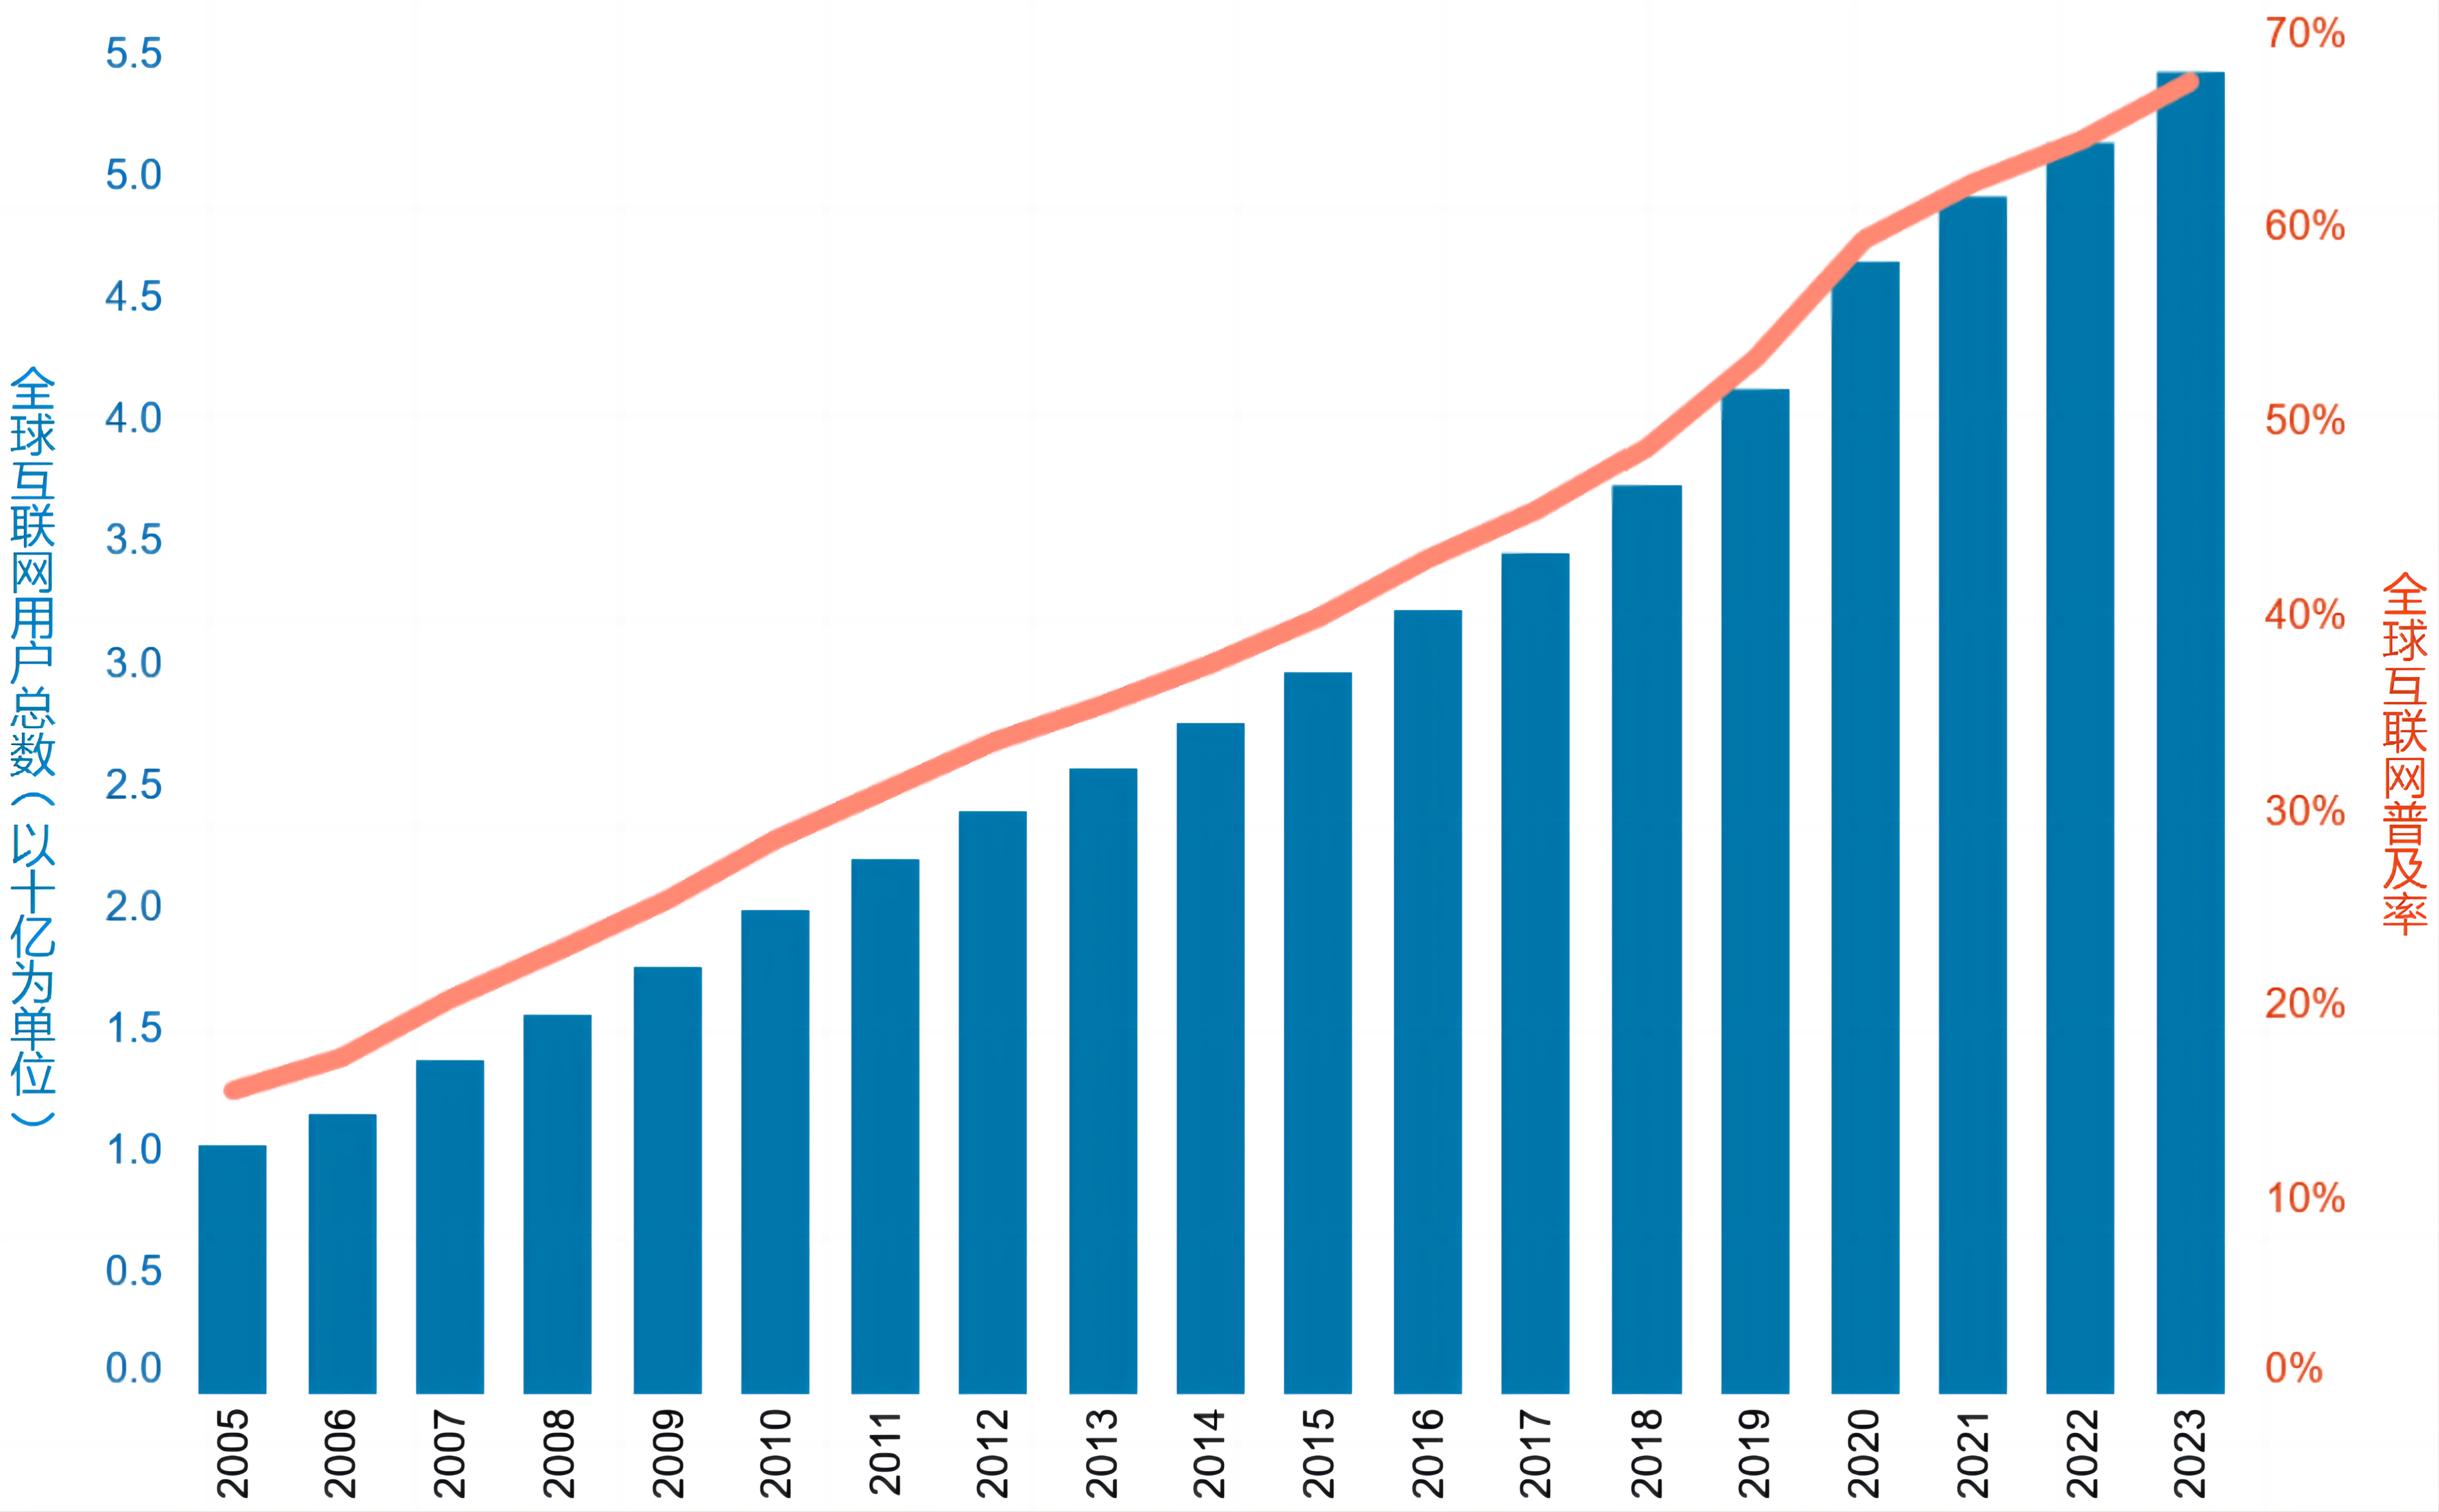
\includegraphics[width = 0.8\textwidth]{individula_using_internet.png}
    \caption{全球网民数量及普及率变化\cite{fig-itu2023}}
    \label{fig:individula_using_internet}
\end{figure} 


尽管互联网规模的扩大为社会经济和科技进步提供了强大的推动力,并为全人类带来了前所未有的便利,但它却是一把双刃剑,伴
随而来的是一系列隐患和威胁,对我们的生活和安全、甚至是国家的稳定都构成了严重的威胁。
2021年,未知攻击者窃取GoDaddy源代码并在其服务器上安装恶意软件,影响了120万Managed WordPress客户的个人信息。
2022年12月,PayPal遭到凭证填充攻击,攻击者通过尝试使用从其他网站数据泄露中获得的用户名和密码对,成功访问了34,942个账户。
2023年5月末,由Clop勒索软件团伙发起了MOVEit攻击。这次攻击利用了Progress MOVEit文件传输工具的关键漏洞,影响了
2,667个组织和近8400万个人,MGM也因此事件估计损失了1亿美元​。此事件被认为是2023
年范围最广的攻击之一,也是近年来最大的数据盗窃事件之一。图~\ref{fig:daily_web_application_attacks}~展示了Akamai关于2022年
与2023年网络攻击每日统计数量。
这些数据表明,随着互联网的广泛普及,网络攻击者日益有组织、专业化,新型网络攻击层出不穷,其特性日益高维、复杂,难以识别。


% 这些原因最终将导致网络攻击变得更加具有破坏力且难以被识别,网络安全形式将变得比以往更加严峻。

\begin{figure}[htbp]
  \centering
  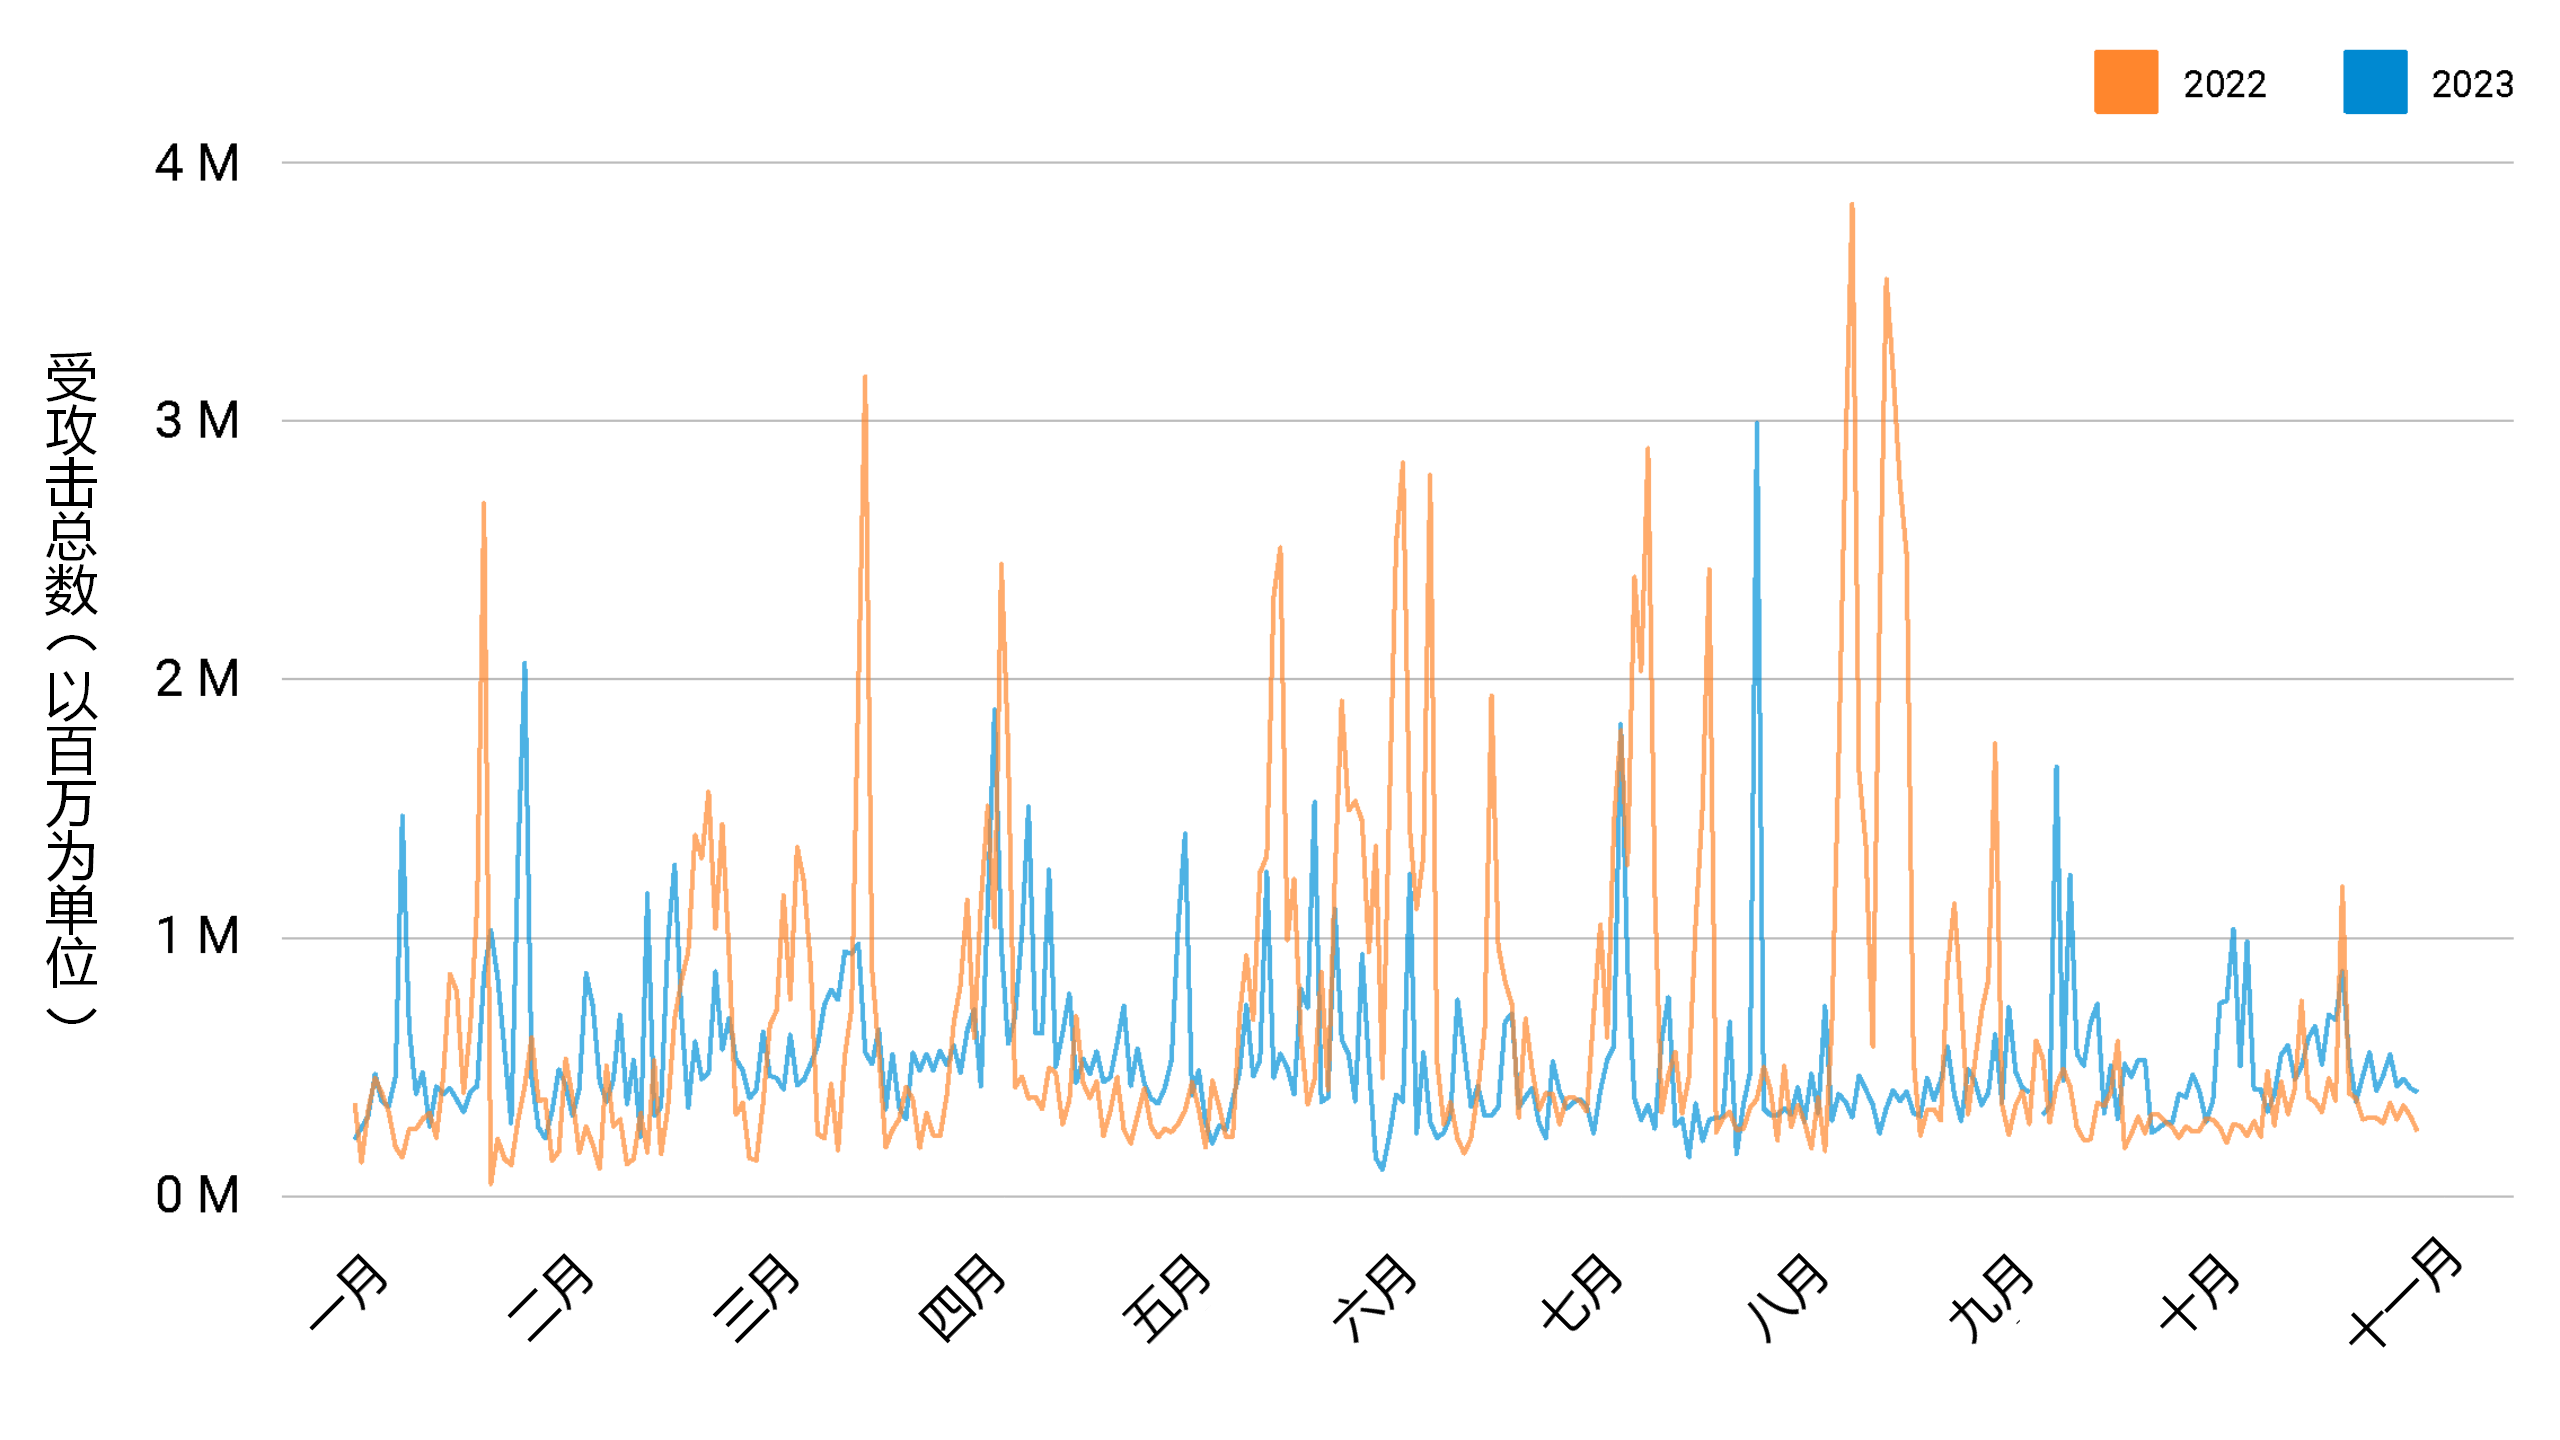
\includegraphics[width = 0.8\textwidth]{daily_web_application_attacks.png}
  \caption{2022年与2023年网络攻击每日统计数量\cite{akamai}}
  \label{fig:daily_web_application_attacks}
\end{figure}

% 网络攻击如此猖獗的原因除了互联网的普及以及网络攻击人员组织化、专业化这些因素之外,
% 网络本身的设计缺陷同样也是一个重要的因素。由于Internet数据传输采用无连接的逐跳转发模式,使
% 网络节点之间的数据包在网络层传输时仅以目的IP进行寻址转发,由此可能导致网络中的恶意节点伪造数据包中源端的IP地址以欺骗目的节点进行非
% 法通信窃取目的端用户的相关信息,导致了基于源地址欺骗类型的网络攻击行为的出现,如MITM、
% 洪泛攻击、反射式攻击、DoS/DDoS攻击等\cite{zhen2022}。攻击数据包中的源地址字段一旦被伪造,就使得识别数据包的来源变得复杂。互联网的无状态
% 特性几乎使得识别攻击的真正来源变得不切实际\cite{singh2016}。这一问题除了导致网络攻击难以
% 被根除之外,还可能引发其他恶意行为,例如恶意用户冒充目标用户的身份,触发运营商或其他服务提供
% 商的管理规则,进而危害目标主机的声誉和利益。解决这个问题对于网络生态系统的安全至关重要。\par

% 随着网络攻击的不断演进,研究者们也在不断采取新的措施来应对这些挑战。从
% 早期的防火墙和反病毒软件的部署,到现在的机器学习和人工智能技术的应用,
% 网络安全领域经历了快速的发展。在20世纪90年代,随着互联网的普及,网络攻击开始成为一个严重的问题。研究    借记卡  
% 者们首先采取的措施是开发和部署防火墙\cite{Ioannidis2000DistributedFirewall}
% 和反病毒软件\cite{Cohen1983},这些基本工具在当时对抵御攻击起到了一定
% 的作用。进入21世纪,随着攻击手段的不断升级,单纯依靠防火墙和反病毒软件已经无法满
% 足防御需要。因此,研究者开始探索新的防御技术。2000年代中期,随着云计算的兴起,
% 研究者开始开发基于云的安全服务\cite{Hashizume2013AnalysisSecurityCloud},
% 这些服务可以提供更灵活、更强大的防御能力。到了2010年代,随着大数据和人工智能技术的发展,研究者开始利用这些技术来提升网络安全。
% 通过分析海量的网络数据,机器学习算法可以识别出复杂的攻击模式,提前预警可能的安全威胁。\par



面对当前日益严峻的网络安全形势,有效识别和应对不断涌现且特征维度持续攀升的新型网络攻击,对于确保网络安全具有不可估量的重要意义。
虽然现有的网络攻击检测技术相比过去已有显著进步,但面对复杂多变的网络环境,仍存在诸多挑战。
首先,海量流量数据日益高维化、复杂化,其多维特征使得单一的检测维度难以全面捕捉。
因此,网络攻击检测模型的准确率受到限制。
若能从多个维度综合分析流量数据,必将进一步提升检测的准确度。
其次,当前的异常流量检测模型大多依赖于静态数据集,难以适应网络环境的动态变化。
特别是随着新型网络攻击的不断涌现,模型的检测性能往往大幅下降。
因此,设计一个既能保持高检测准确率又能灵活应对新型攻击的模型成为迫切需求。
最后,现有的异常流量检测模型主要停留在被动检测层面,缺乏主动处理能力和源头解决方案。
例如,在面对DDoS攻击时,若模型仅依赖源IP地址过滤异常流量,一旦攻击者频繁更换僵尸节点的IP地址,模型将不堪重负,甚至崩溃。
因此,为模型设计一套有效的防护机制,从源头上解决异常流量问题,成为当务之急。
% 虽然这些技术在互联网发展5的各个环节对网络安全的防护都具备一定的积极作用,
% 但这些方法却没有考虑到TCP/IP协议本身存在的缺陷,即:网络在运行过程中通常不会对
% 数据包源地址的真实性进行验证。这意味着,即便现有算法能够准确地识别并阻止网络攻击,然而,
% 一旦攻击者变更其源IP地址,系统就必须重新进行攻击检测。当攻击者发送大量带有虚假IP地址的
% 数据包时,防护系统的表现效果将大打折扣。为了应对这个问题,IP回溯技术应运而生。
% 该技术通过受害者主机与多个网络设备的协作,利用网络运行所产生的信息,对攻击路径进行重构,
% 从而揭露攻击源的实际位置。\par 

% 在众多的网络回溯方法中,概率包标记法以其简单、灵活、易于部署及无需人工参与的特点脱颖而出,同时它还支持事后分析,为网络安全领域提供了重要的技术支持。
% 然而,概率包标记法在速度方面存在明显的短板,路径重构过程中需要收集大量的数据包,这无疑增加了时间成本和处理复杂性。
% 针对概率包标记法速度慢的问题,本文提出一种基于路由器接口号分组的概率包标记法。
% 该方法利用路由器接口号作为标记信息,提高了标记空间的利用率。
% 通过该方法,单个数据包便能携带一组标记信息,显著减少所需收集的数据包数量,进而大幅提升路径重构的速度与效率。\par

% 此外,当前的网络方案多依赖于静态的数据集,这在动态变化的网络环境中显然是不够的。
% 为了应对这一挑战,本文还提出一个基于多模态特征融合的增量学习方案。
% 该方案结合残差网络与双向门控循环单元的优势,充分挖掘网络数据的时空特征,并通过增量学习的方式,不断适应网络环境的变化。
% 这种方案不仅提高了检测的准确性,还增强了模型的适应性,为动态网络环境下的网络安全提供了有力保障。\par


% 因此,本文基于这一愿景,设计了一个网络攻击检测及溯源系统,
% 该系统能够在检测到异常流量时,精确地确定攻击主机的实际地址。

\section{国内外研究现状}
% 在本小节中,我们将会对网络溯源相关的研究现状进行分析。
% 一般情况下,溯源只有在系统检测到攻击时才会进行网络溯源。
% 因此本文的工作将会围绕网络溯源和网络攻击检测这两个研究方向共同进行。
% 此处的研究现状也会围绕这两个研究方向分别展开叙述。

% \subsection{网络溯源研究现状}
% IP追踪方案可以根据用于收集追踪信息的底层方法进行分类。这些方法在部署策略、存储需求、
% 信息收集算法等方面可能有所不同。下面给出了几种常见的溯源方法\cite{singh2016}。
% 这几种方法的性能表较如图~\ref{tb:compare_approch}~所示。

% \textbf{链路测试法:}链路测试会对所有上游链路进行递归的分析,直到到达源点为止,以确定传递攻击数据包的链路。
% 从最接近受害者的路由器开始,直到攻击者的源路由器。图~\ref{fig:linktest}~展示了此方法的基本原理。2000年,Burch提出了基于这一
% 原则的第一个IP回溯方案\cite{Burch2000Tracing}。随后是一些基于链接测试的回溯方案
% \cite{HamediHamzehkolaie2012DOSTraceback,ShiYang2005DDoSDefense,
% ThingSlomanDulay2008DDoSDetection}。
% 链路测试方案有两种:输入调试和控制洪水。

% \begin{figure}[htbp]
%   \centering
%   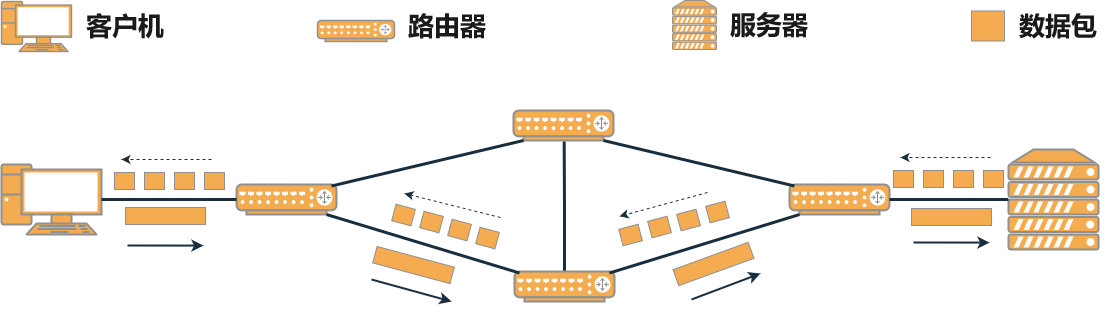
\includegraphics[width = 0.8\textwidth]{linktest.drawio.png}
%   \caption{链路测试法原理}
%   \label{fig:linktest}
% \end{figure}

% \textbf{输入调试法:}在输入调试法中每个路由器都有能力根据特定的分组特征来确定其传入的链路。受到攻击的
% 受害者可以构建一个攻击数据包签名,并将其发送到上游路由器。然后,路由器可以根据
% 接收到的攻击包签名递归地调查其上游链路,从而识别出攻击者。下面列出了这种方法的优缺点。
% \begin{itemize}
%   \item 优点:
%     \begin{itemize}
%     \item 与现有的协议和基础设施相一致。
%     \item 为增量部署提供了良好的支持。
%     \item 在网络流量上的带宽开销很小。
%   \end{itemize}
% \item 缺点:
%   \begin{itemize}
%     \item 不适合DDoS环境。
%     \item 依赖于isp之间的合作。
%     \item 跟踪系统只在攻击时运行。
%   \end{itemize}
% \end{itemize}

% \textbf{控制泛洪法:}在控制泛洪法中,受害者利用预定义的ISP地图迭代地将数据包淹没其上游路由器,
% 并同时确定攻击强度的变化。这个递归过程可以在每个上游级别上显示攻击源。下面列
% 出了这种方法的优缺点。
% \begin{itemize}
%   \item 优点:
%     \begin{itemize}
%       \item 与现有的协议和基础设施相一致。
%       \item 支持简单和增量的实现。
%     \end{itemize}
%   \item 缺点:
%     \begin{itemize}
%       \item 追踪只在持续的攻击中进行。
%       \item 需要具备网络拓扑结构的先验知识。
%       \item 对DDoS攻击无效。
%     \end{itemize}
% \end{itemize}

% \textbf{消息传递法:}消息传递在向目标传输回溯相关信息方面提供了更大的灵活性。主要采用Taylor等人
% 提出的基于互联网控制消息协议(ICMP)的方案\cite{Taylor2014ICMP}。
% 在该方案中,每个
% 路由器概率地生成一个称为跟踪包或iTrace消息的ICMP包,该包负责携带要用作回
% 溯过程的输入的信息,它可能包含下一跳和上一跳信息、
% 时间戳、MAC地址等参数。在攻击期间,成千上万个这样的iTrace数据包
% 有助于成功的回溯操作。但是,为了避免由这些消息造成的网络流量开销,消息生成的
% 概率通常会保持在可容忍的限制下。Hsu和Chiueh
% \cite{Hsu2003TrafficSourceIdentification}和Wang和Schulzrinne
% \cite{WangSchulzrinne2004DoS,WangSchulzrinne2004ReflectiveDoS}所做的工作
% 就是此类方法的代表。图~\ref{fig:messaging}~展示了消息传递法的基本原理。
% 下面列出了这种方法的优缺点。
% \begin{itemize}
%   \item 优点:
%     \begin{itemize}
%       \item 支持具有低ISP合作能力的增量部署。
%       \item 与现有的协议和基础设施相一致。
%       \item 允许对攻击后进行分析。
%     \end{itemize}
  
%   \item 缺点:
%     \begin{itemize}
%       \item 如果缺乏身份验证支持,很容易被攻击者滥用。
%       \item 由于生成额外的数据包而产生网络流量开销。
%     \end{itemize}

% \end{itemize}

% \begin{figure}[htbp]
%   \centering
%   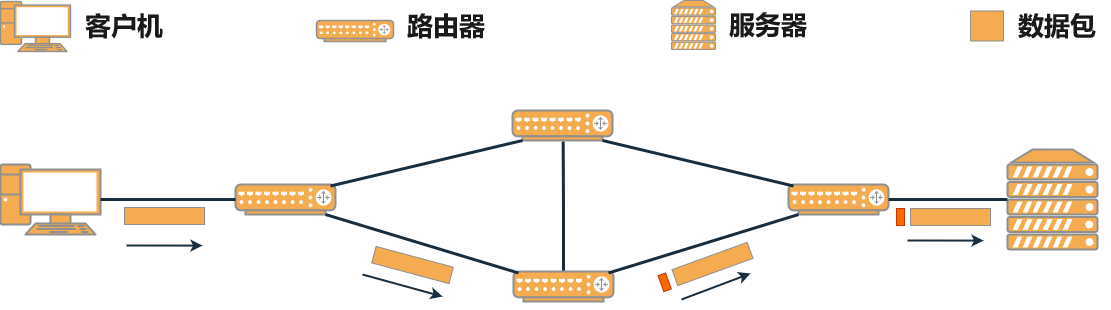
\includegraphics[width = 0.8\textwidth]{messaging.drawio.png}
%   \caption{消息传递法原理}
%   \label{fig:messaging}
% \end{figure}


% \textbf{数据包标记法:}数据包标记法背后的关键思想是利用数据包本身来记录路由信息。其原理如图~\ref{fig:packet_marking}~所示。
% 受害者使用这些信息来探索该数据包所遍历的路径。标记数据包既可以包含完整的编码路由信息,也可携带由中间路由器嵌入的
% 一个或多个标记。受害者可以识别所有收集到的标记数据包,并利用
% 存储在标记字段中的信息来跟踪攻击源。概率分组标记(PPM)和确定性分组标记
% (DPM)是两种最突出的标记方案\cite{Burch2000Tracing}。这两种方案是现有
% 文献中许多基于标记的方案的基础。~\ref{fig:ipv4_header}~展示了数据包头部字段被用来
% 填充标记信息的使用情况。
% 为避免数据包头过载以及降低路径重构过程中的误报率的需求,数据包标记法需要适当的标记编码方案,
% 此外,数据包标记法有三种主要的标记策略:节点附加法、节点采样法、边采样法\cite{Alenezi2011}。

% \begin{figure}[htbp]
%   \centering
%   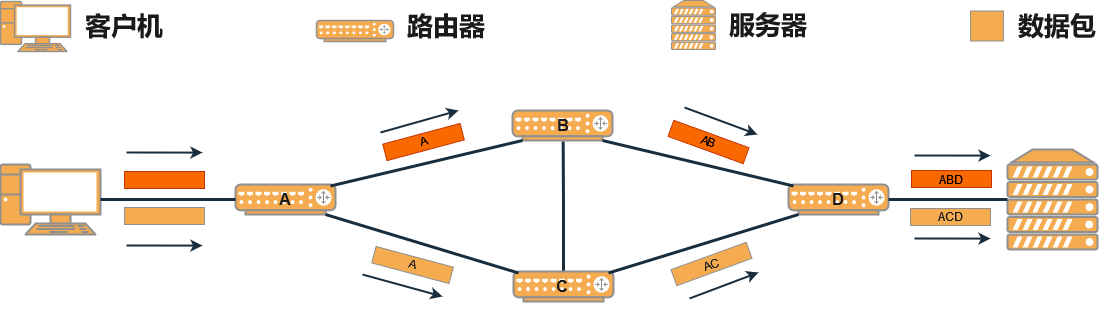
\includegraphics[width = 0.8\textwidth]{packetmarking.drawio.png}
%   \caption{数据包标记法原理}
%   \label{fig:packet_marking}
% \end{figure}

% \textbf{节点附加法:}在节点附加法中路由器的信息将会作为标记被逐个追加到原始IP包头中
% \cite{Amin2006,Min2003}。
% 这种机制通过在单个数据包中携带多个路由信息简化了标记过程。因此这种方法仅仅依靠单个标记包
% 便能确定一条完整的路径。但此种方法由于增加了过多的标记字段导致高网络带宽开销。这一缺陷也
% 限制了此种方法的应用。

% \textbf{节点采样法:}一个单个的标记数据包只会携带单个路由节点的标记信息,这就意味着当
% 路由器对将自身路由信息写入标记数据包时会覆盖掉之前的信息。不过这也导致导致标记策略的灵活
% 性降低。节点采样法的标记信息通常包括路由器的IP地址。也有许多方案为路由器分配颜色、身份
% 编号或其它特定的标记功能\cite{Jin2009,Liu2006}。

% \textbf{边采样法:}边采样法涉及到边缘信息的编码,如起始、结束等,而不是再针对单个节点
% 信息的操作。其他常见的边缘信息属性包括边缘权重、颜色、身份编号等。除了这些属性外,
% 巧妙地使用距离字段,能够让方案在不需要预先了解互联网拓扑的情况下具备构建攻击路径的能力。
% 以下列出了这种方法的优点和缺点。
% \begin{itemize}
%   \item 优点:
%   \begin{itemize}
%     \item 现有网络基础设施兼容。
%     \item 与其他方法相比,实施简单灵活。
%     \item 适用于DDoS攻击。
%     \item 需要的ISP支持最少。
%   \end{itemize}
%   \item 缺点:
%   \begin{itemize}
%     \item 由于在许多追踪方案中过载标识字段,导致数据包碎片化问题。
%     \item 有时可能产生高误报结果。
%     \item 需要修改现有协议来实现标记过程。
%     \item 追踪准确性取决于受害节点收到的标记数据包的数量。
%   \end{itemize}
% \end{itemize}




% \begin{figure}[htbp]
%   \centering
%   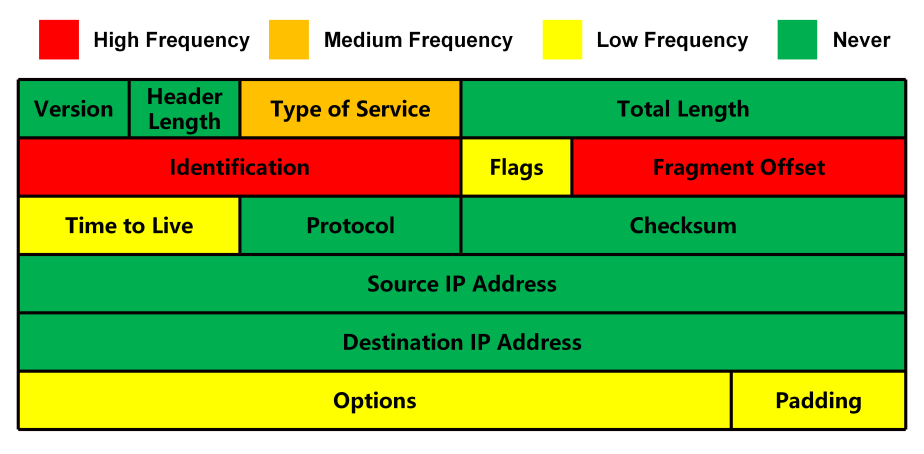
\includegraphics[width = 0.8\textwidth]{ipv4_header.png}
%   \caption{标记过程中使用的IPv4头部字段}
%   \label{fig:ipv4_header}
% \end{figure}


% \textbf{路由器日志记录法:}
% 记录法旨在将数据包摘要存储在中间路由器上。
% 然后当受害者服务器进行攻击路径重构时便可使用这些路由器上存储的信息来确定网络路径。
% 日志记录法的原理如图~\ref{fig:loggging}~所示。
% 尽管这种方法的回溯效果很不错,因为它可以使用单个数据包完成攻击路径重构,但它的一个主要缺点是:它将会给路由器带来巨大的存储开销。
% 因此,它的部署一直是一个挑战。
% Snoeren等人\cite{Snoeren2001}提出了一种基于哈希的IP追踪方法,称为源路径隔离引擎,以实际实现基于日志的IP追踪。
% 他们的方法使用了一种称为布隆过滤器的空间高效数据结构,显著减少了路由器存储数据包摘要的存储开销。
% Kai等人\cite{Kai2009}、Hilgenstieler等人\cite{Hilgenstieler2010}都对此方法提出了改进进一步增强了性能。
% 这种方法的优点和缺点如下。
% \begin{itemize}
%   \item 优点:
%   \begin{itemize}
%     \item 与协议和现有基础设施兼容。
%     \item 支持攻击后分析。
%     \item 允许追溯单个数据包。
%     \item 网络流量开销可忽略。
%   \end{itemize}
%   \item 缺点:
%     \begin{itemize}
%       \item 高内存和处理要求。
%       \item ISP合作的隐私问题对这种方法构成问题。
%       \item 需要及时进行追踪,因为路由器会定期刷新以前记录的信息。
%     \end{itemize}
% \end{itemize}

% \begin{figure}[htbp]
%   \centering
%   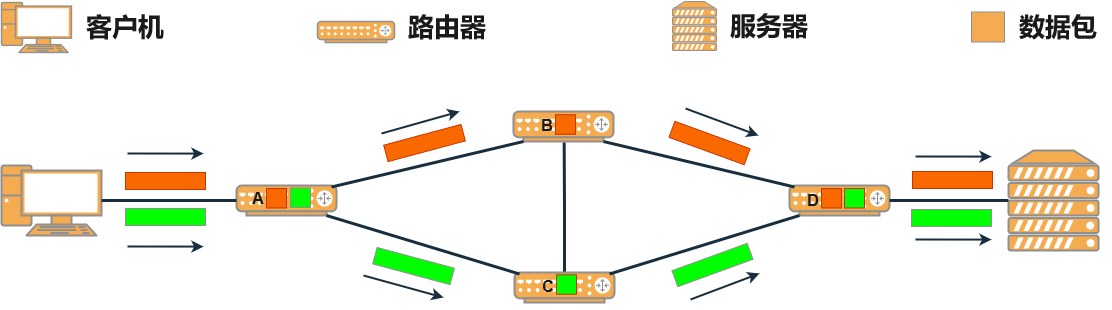
\includegraphics[width = 0.8\textwidth]{logging.drawio.png}
%   \caption{路由器日志记录法原理}
%   \label{fig:loggging}
% \end{figure}

% \textbf{覆盖法:}一个覆盖网络主要由用来跟踪路由的专用路由器组成,这些专用路由器被称为跟踪路由器。
% 这些路由器的主要职责是监控流量,当检测到攻击时,覆盖网络将发出命令指示流量通过这些专用路由器。
% 然后,这些路由器检查通过它们的流量,并提取用于追踪来源的信息。图~\ref{fig:overlay}~Stone提出了这样一个系统,称为CenterTrack,它通过分析通过中心化跟踪路由器的流量来提供追踪服务\cite{stone2000centertrack}。
% Castelucio等人\cite{castelucio2009aslevel}和Tian等人\cite{tian2011easytrace}提出的工作也采用了基于覆盖的方法进行IP追踪。这种方法的优点和缺点如下。
% \begin{itemize}
%   \item 优点:
%   \begin{itemize}
%     \item 提供准确的追踪结果。
%     \item 有效处理DDoS攻击。
%     \item 客户端免于执行追踪过程。
%   \end{itemize}

  
%   \item 缺点:
%   \begin{itemize}
%     \item 实施成本高。
%     \item 缺乏对渐进式部署的支持。
%     \item 跟踪路由器本身可能成为DDoS攻击的目标。 
%   \end{itemize}

% \end{itemize}

% \begin{figure}[htbp]
%   \centering
%   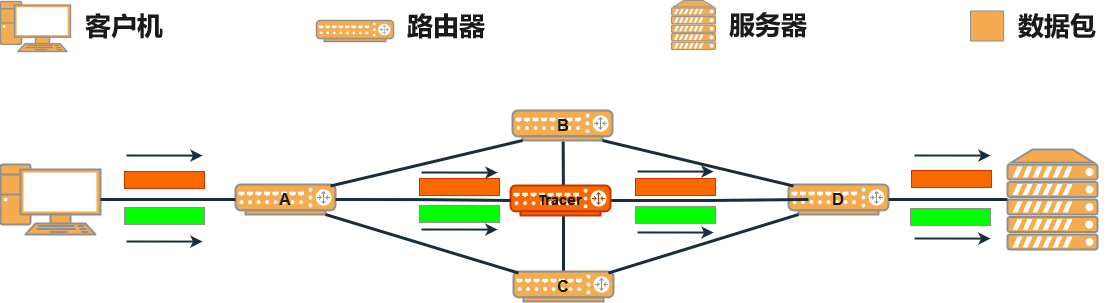
\includegraphics[width = 0.8\textwidth]{overlay.drawio.png}
%   \caption{覆盖法原理}
%   \label{fig:overlay}
% \end{figure}

% \textbf{模式分析法:}在攻击进行时,路由器可以提取流量模式信息,这些信息可以用于溯源,如Xiaofeng等人\cite{xiaofeng2004mechanism}、
% Chen等人\cite{chen2006tracing}和Lai等人\cite{lai2008antbased}所提出的。在这种方法中所有参与溯源的路由器以分布式方式相互合作,收集流量信息并追踪攻击源。
% 这使得受害者免于执行追踪任务,这被认为是这种方法的一个主要优点。
% 这种方法的优点和缺点如下。
% \begin{itemize}
%   \item 优点:
%     \begin{itemize}
%       \item 客户端免于执行追踪过程。
%       \item 追踪过程的分布式处理。
%       \item 提供了改善的可扩展性。
%     \end{itemize}
%   \item 缺点:
%     \begin{itemize}
%       \item 由于持续的流量监控,路由器处理开销大。
%       \item 在DDoS攻击中,随着攻击流量的增加,复杂性增加。
%     \end{itemize}
% \end{itemize}

% \begin{table}[htbp]
%   \caption{IP回溯方法性能比较}
%   \label{tb:compare_approch}
%   \centering
%   \begin{tabular}{ccccccc}
%   \toprule
%   {\heiti 回溯方法} & {\heiti 管理开销} & {\heiti 网络开销} & {\heiti 路由器开销} & {\heiti ISP合作} & {\heiti 假阳率} & {\heiti 时间开销}\\
%   \midrule
%   链路测试法 & Moderate &  Low & Moderate & Collaborative & High & Long\\
%   数据包标记法 & Low & Low & Low & Noncollaborative & Low & Long\\
%   路由器日志记录法 & High & Low & High & Collaborative & Low & Middle\\
%   消息传递法 & Low & Low & Low & Noncollaborative & Very Low & Long\\
%   覆盖法 & Low & Low & High & Collaborative & Low & Middle\\
%   模式分析法 & Low & Moderate & High & Collaborative & Low & Middle\\
%   \bottomrule
%   \end{tabular}
%   \end{table}


% \subsection{网络攻击检测研究现状}
异常流量检测的研究主要可以分为基于传统机器学习方法和基于深度学习的方法。\par
1)基于机器学习的方法\par
在18世纪50年代,机器学习技术还处于其早期探索阶段,标志性事件之一是1952年亚瑟·萨缪尔开发的能够在IBM 701上运行的西洋跳棋程序,这是机器学习应用的早期例证。
进入60年代,随着最近邻算法(Nearest Neighbor Algorithm)\cite{cover1967nearest}的提出,模式识别和机器学习技术开始取得初步发展。
随后的几十年见证了机器学习技术的快速成熟,诸如决策树\cite{Quinlan1986}、支持向量机(SVM)\cite{Cortes1995}、随机森林\cite{Breiman2001}等算法相继被提出。
这些算法的发展不仅推动了机器学习领域的进步,也为后来的攻击检测技术打下了坚实的基础。
特别是,支持向量机(SVM)和随机森林等算法开始被集成到入侵检测系统中,标志着基于机器学习方法的网络攻击检测技术的蓬勃发展\cite{Mukkamala2002}。
这些基于机器学习的攻击检测技术,具体可分为有监督学习和无监督学习。



有监督的机器学习攻击检测技术主要依赖于预先标记的数据集来训练模型,使其能够识别和区分正常行为与恶意行为。
这种技术通常涉及将数据集分为训练集和测试集,其中训练集用于训练模型,而测试集则用于评估模型的性能。
有监督学习的关键在于拥有大量已经被标记为正常或攻击的样本,这些样本用于让机器学习算法“学习”识别攻击行为的模式。
在有监督的机器学习攻击检测领域,主要可以分为以下几种类型:基于异常的检测、基于签名的检测、以及基于行为的检测。
每种类型都有其独特的方法和应用场景。


基于异常的检测技术通常依赖于机器学习模型来识别与已知正常行为模式显著偏离的行为。
早期的工作可以追溯到1990年代,其中Lee和Stolfo等人\cite{lee1998dataMining}在1998年的研究中对异常检测技术做出了重要贡献,提出了使用数据挖掘技术来识别网络入侵的方法。
之后Schonlau等人在2001年提出的MASQUE模型,旨在通过监视用户行为来检测异常,进而识别潜在的攻击活动。

基于签名的检测技术则是基于已知攻击的特定模式或签名来识别攻击。
这种方法的关键在于建立一个广泛的攻击特征库。
Kumar和Spafford\cite{kumar1994adep}在1994年的研究中,通过他们的工作ADEPTS,为基于签名的检测技术做出了显著贡献,发展了一种基于异常检测和签名匹配的混合方法来提高检测的准确性。

基于行为的检测技术关注于分析系统或网络中的行为模式,以识别潜在的恶意活动。
这种方式侧重于学习和理解系统或用户的正常行为模式,以便任何偏离这些模式的行为都可能被标记为恶意的。
在这个方向上,Anderson等人\cite{anderson1995userBehavior}在1995年提出了一种基于用户行为分析的入侵检测系统,该系统通过学习正常的用户行为模式来识别异常活动。
这种类型的研究在2000年代初期得到了加强,其中Forrest等人\cite{forrest1996selfImmune}在自身免疫系统的概念上的工作为基于行为的检测提供了理论基础,推动了基于行为的检测技术的发展。



无监督的机器学习攻击检测技术不依赖于预先标记的数据集,而是通过分析数据中的模式、异常或者关系来识别可能的恶意行为。
这种技术尤其适用于那些标签数据稀缺或者完全没有标签的情况,允许模型自行发现数据集中的结构。
在无监督学习领域,主要的攻击检测方法包括聚类、异常检测以及密度估计等。

聚类是一种常见的无监督学习技术,通过将数据分成由相似对象组成的多个组来工作。
在攻击检测中,聚类方法可以用来识别出不寻常的数据点集合,这些集合可能代表了恶意活动。
Portnoy等人\cite{portnoy2001clustering}在2001年的研究中通过聚类技术成功识别出异常行为,展示了聚类方法在入侵检测中的有效性。

异常检测技术在无监督学习中也占有一席之地,与有监督学习中的基于异常的检测技术相似,但不依赖于预标记的数据。
Eskin等人\cite{eskin2002anomaly}在2002年的工作中提出了一种基于异常检测的入侵检测系统,该系统能够在没有任何先验知识的情况下识别攻击行为。

密度估计方法,如局部异常因子(LOF)算法,通过评估数据点在其邻域的密度来识别异常点。
这种方法适用于发现那些在低密度区域的数据点,可能指示着异常或攻击行为。
Schubert等人\cite{schubert2014local}在2014年对LOF算法进行了改进,以增强其在检测网络入侵方面的性能。

虽然传统机器学习方法在处理一些简单的异常流量检测问题上相对方便,但在应对复杂、非结构化以及高维度流量特征数据时很难有效地学习到深层次的特征。
因此,越来越多的研究人员开始采用深度学习方法,以提高网络异常流量检测的效率和准确性。\par

2) 基于深度学习的方法\par
深度学习是机器学习的一个分支,它通过使用具有多个隐藏层的神经网络来模拟人类大脑的工作方式,从而解决复杂的模式识别问题。
1943年,McCulloch和Pitts提出了最早的神经网络模型。
1986年,Rumelhart, Hinton和Williams重新引入了反向传播算法,使得训练多层神经网络成为可能。
2006年,Hinton和他的学生提出了深度置信网络,标志着深度学习的复兴。
随后,在2010年代初,随着深度学习技术的发展,研究人员开始探索其在网络安全和攻击检测中的应用。
深度学习在处理和分析大规模复杂数据方面的能力,使其成为提高攻击检测性能的有力工具。

基于深度学习的攻击检测技术,根据其学习和推理的方式,可以大致分为生成式方法、判别式方法和混合式方法。


生成式方法旨在学习数据的联合分布$P(X,Y)$,其中$X$是输入数据,$Y$是标签。
这种方法通过模拟数据生成过程来理解和识别正常与异常模式。
在攻击检测中,生成式模型可以用于生成与真实数据分布相似的样本,从而帮助识别潜在的攻击行为。
典型的生成式模型包括深度信念网络(DBNs)和生成对抗网络(GANs)。
2014年,Goodfellow等人提出了生成对抗网络(GANs)\cite{goodfellow2014generative},这是一种强大的生成式模型,能够生成与真实数据几乎无法区分的数据样本。
在攻击检测领域,GANs被用于生成攻击数据,以帮助训练模型更好地识别和适应新的攻击类型。
2015年,An和Cho探索了使用变分自编码器(VAE)进行异常检测的方法\cite{an2015variational}。
该方法通过计算输入数据的重构概率来识别异常,展示了VAE在复杂数据集上进行无监督异常检测的潜力。


判别式方法专注于学习从输入数据到标签的条件概率分布$P(Y∣X)$。
这类方法通过区分不同类别的数据特征来进行分类或预测。
在攻击检测应用中,判别式模型,如卷积神经网络(CNNs)和循环神经网络(RNNs),被广泛用于直接识别各种类型的网络攻击,因为它们能够有效处理和分析大量的网络数据。
2015年,Saxe和Berlin展示了如何使用深度CNN来检测恶意软件\cite{saxe2015deep}。
他们通过将二进制文件转换为二维图像,然后使用CNN进行特征学习和分类,有效提高了恶意软件检测的准确率。
2019年,在论文中\onlinecite{staudemeyer2019applying},Staudemeyer和Morris展示了如何利用LSTM网络来检测DDoS攻击。
他们利用RNN的时间序列学习能力,有效识别了网络流量中的异常模式。

混合式方法结合了生成式和判别式方法的优点,以提高模型的泛化能力和准确性。
这种方法通常涉及使用生成模型来增强数据或特征,随后通过判别模型进行精确的分类或检测。
混合式方法在攻击检测中特别有用,因为它们可以通过生成式组件来理解和模拟攻击行为的复杂性,同时利用判别式组件的强大分类能力来准确识别攻击。
2018年,Li及其团队提出了MAD-GAN\cite{li2018mad},一种结合生成对抗网络和深度学习模型的方法来检测时间序列数据中的多变量异常。
这种方法通过GAN生成的模拟异常数据来训练深度学习模型,从而提高了模型对新型攻击行为的检测能力。
2019年,Feng及其团队提出了一种结合自编码器和卷积神经网络的方法来检测物联网(IoT)网络中的异常行为\cite{feng2019deep}。
该方法首先利用自编码器学习正常网络流量的特征表示,然后使用CNN对流量进行分类,有效识别了异常模式。


\section{论文研究内容}
% 在众多的网络回溯方法中,数据包标记法与其他方法相比具有简单、灵活、易于部署、无需人工参与、支持事后分析等优点,但此类方法仍然存在一些局限性和改进的空间。
% 在PPM方案中,完成路径覆盖进行路径重构所需要的数据包数量与受害者服务器到攻击者主机的距离d成指数关系。
% 因此当d特别大时,路径重构的过程是十分缓慢的。DPM方案虽然可以弥补PPM存在的缺陷,但此方案需要将整条路径上的路由信息(通常为IP地址)追加到数据包头部,这将会导致IP包头过大而带来一系列问题。
% 因此本文首先综合考虑两种方案的优缺点,巧妙地利用路由器接口号的局部性,设计一种改进的数据包标记方案,在不扩大数据包头部的情况下在单个数据包上对多个路由器进行标记成为可能。\par

% 尽管当今网络攻击检测技术已取得了显著进步,但仍存在诸多不足。
% 首先,当今的检测模型通常只关注流量数据的单一维度特征,当面对维度不断攀升的流量数据时,无法充分应对日益复杂的网络攻击,模型的检测能力将会有所下降。
% 针对上述问题,本文提出了一种基于残差网络与双向门控循环单元的多模态特征融合模型。
% 该模型不仅能够深入挖掘数据中的空间特征与时序特征,还能通过综合分析这些特征,做出更为精准的决策。

% 另外,当前检测技术多依赖于静态数据集,难以适应快速变化的网络环境,导致在实际应用中面临诸多挑战。
% 为了应对不断变化的网络环境,本文引入了iCaRL()技术\cite{},使本文所提的模型进在保留对原有知识的基础上实现对新攻击模式的快速学习和适应,从而确保网络安全的持续性和稳定性。
% 最后为了使我们的模型当面对DDoS攻击时能够正常运作并从源头上解决DDoS攻击,本文将为模型提供一套防护技术,当时别到攻击流量后可针对流量进行具体的溯源从源头上对其进行处置。

尽管现有的网络攻击检测技术已经取得了长足的进步,但在实际应用中仍然暴露出不少短板。
首要问题在于,现有的检测模型大多仅聚焦于流量数据的单一维度特征,这在面对日益复杂且多维度的流量数据时显得力不从心,导致模型的检测效能大打折扣。
为了弥补这一不足,本文提出了一种基于残差网络与双向门控循环单元的多模态特征融合模型。
这一模型不仅能够有效挖掘数据中的空间与时序特征,更能通过全面、综合的分析,做出更为精准的判断,从而显著提升检测的准确性和可靠性。
此外,当前的网络攻击检测技术多依赖于静态数据集,这在快速变化的网络环境中显得捉襟见肘,实际应用中面临诸多挑战。
为了应对这一挑战,本文引入了iCaRL技术并基于遗传算法对该技术进行了优化改进,使得所提模型能够在保留原有知识的基础上,迅速学习并适应新的攻击模式,确保网络安全的持续性和稳定性。
最后,为了确保模型在面对DDoS攻击时能够稳定运行,并从根本上解决问题,本文还将为模型设计一套专门的防护技术。
一旦模型识别到攻击流量,我们将为其配备一套专门的机制,能够迅速定位并处理异常流量,从源头上消除威胁,确保模型的稳定运行。
% 其次,尽管机器学习和深度学习技术已广泛应用于网络异常流量检测,但挑战仍然存在,特别是在准确性和未标记数据处理方面的局限性凸显了现有方法的不足。
% 因此,为了能够处理少量标记数据的情况和达到更高的检测精度,以及能够有效挖掘复杂网络数据的深层特征,我们引入了基于遗传算法和增量学习提升的ResNet-BiGRU混合模型。
% 最后,考虑到网络环境中常见的问题,即在运行过程中往往忽略了对数据包源地址真实性的验证,导致攻击者可能利用伪造的IP地址发起攻击。
% 为此,本文会将提出的攻击检测方法与溯源技术相结合,开发一套网络攻击检测及溯源系统。
% 该系统旨在不仅能够准确检测出网络攻击行为,而且能进一步追踪到发起攻击的主机的真实位置,有效应对攻击者使用伪造IP地址的策略。
因此,本文的研究内容及主要贡献如下:\par

1)鉴于当前网络攻击检测技术主要关注流量数据的单一维度,特征挖掘不足,导致异常流量检测精准度有待提升。
为此,本文创新性地提出了一种基于残差网络与双向门控循环单元的多模态特征融合模型。
该模型结合残差网络的强大空间特征提取能力与双向门控循环单元的时序特征分析优势,通过多模态特征融合技术,全面深入地分析流量数据的时空特征,进而提升检测精准度。\par

2)针对当前的网络攻击检测技术大多依赖于静态的数据集,难以适应快速变化的网络环境的问题,
本文引入了iCaRL技术并基于遗传算法对该技术进行了优化改进,使得所提模型能够在保留原有知识的基础上,迅速学习并适应新的攻击模式,确保网络安全的持续性和稳定性。\par

3)为应对DDoS攻击对模型可能造成的严重负担,本文基于数据包标记溯源原理,创新性地设计并提出了一种基于路由器接口号分组的概率标记溯源方法——IGPPM。
该方法充分利用路由器接口号的局部性特点,在不增加数据包大小的情况下,对路径上的一组连续路由器进行有效标记。    d              
这使得单个数据包能够携带更为丰富的路由信息,从而迅速且准确地完成路径溯源工作。
一旦定位到攻击者源头,便能从源头处直接过滤掉攻击流量,有效减轻模型的负担,确保网络的安全稳定。\par

% 该模型充分融合了残差网络在特征提取方面的优势与双向门控循环单元在处理时序数据时的长处,从而实现对流量数据时空特征的深度挖掘。
% 通过综合分析这些特征,模型能够做出更为精准的攻击检测决策。
% 在UNSW-NB15数据集上的实验结果表明,相较于传统机器学习模型以及ResNet、BiGRU等模型,本模型在准确率方面表现出色,为攻击检测任务提供了更加高效和可靠的解决方案。\par



\section{论文组织结构}
本论文一共有5个章节,其组织结构如图~\ref{fig:paper_structure}~所示。
\begin{figure}[htbp]
  \centering
  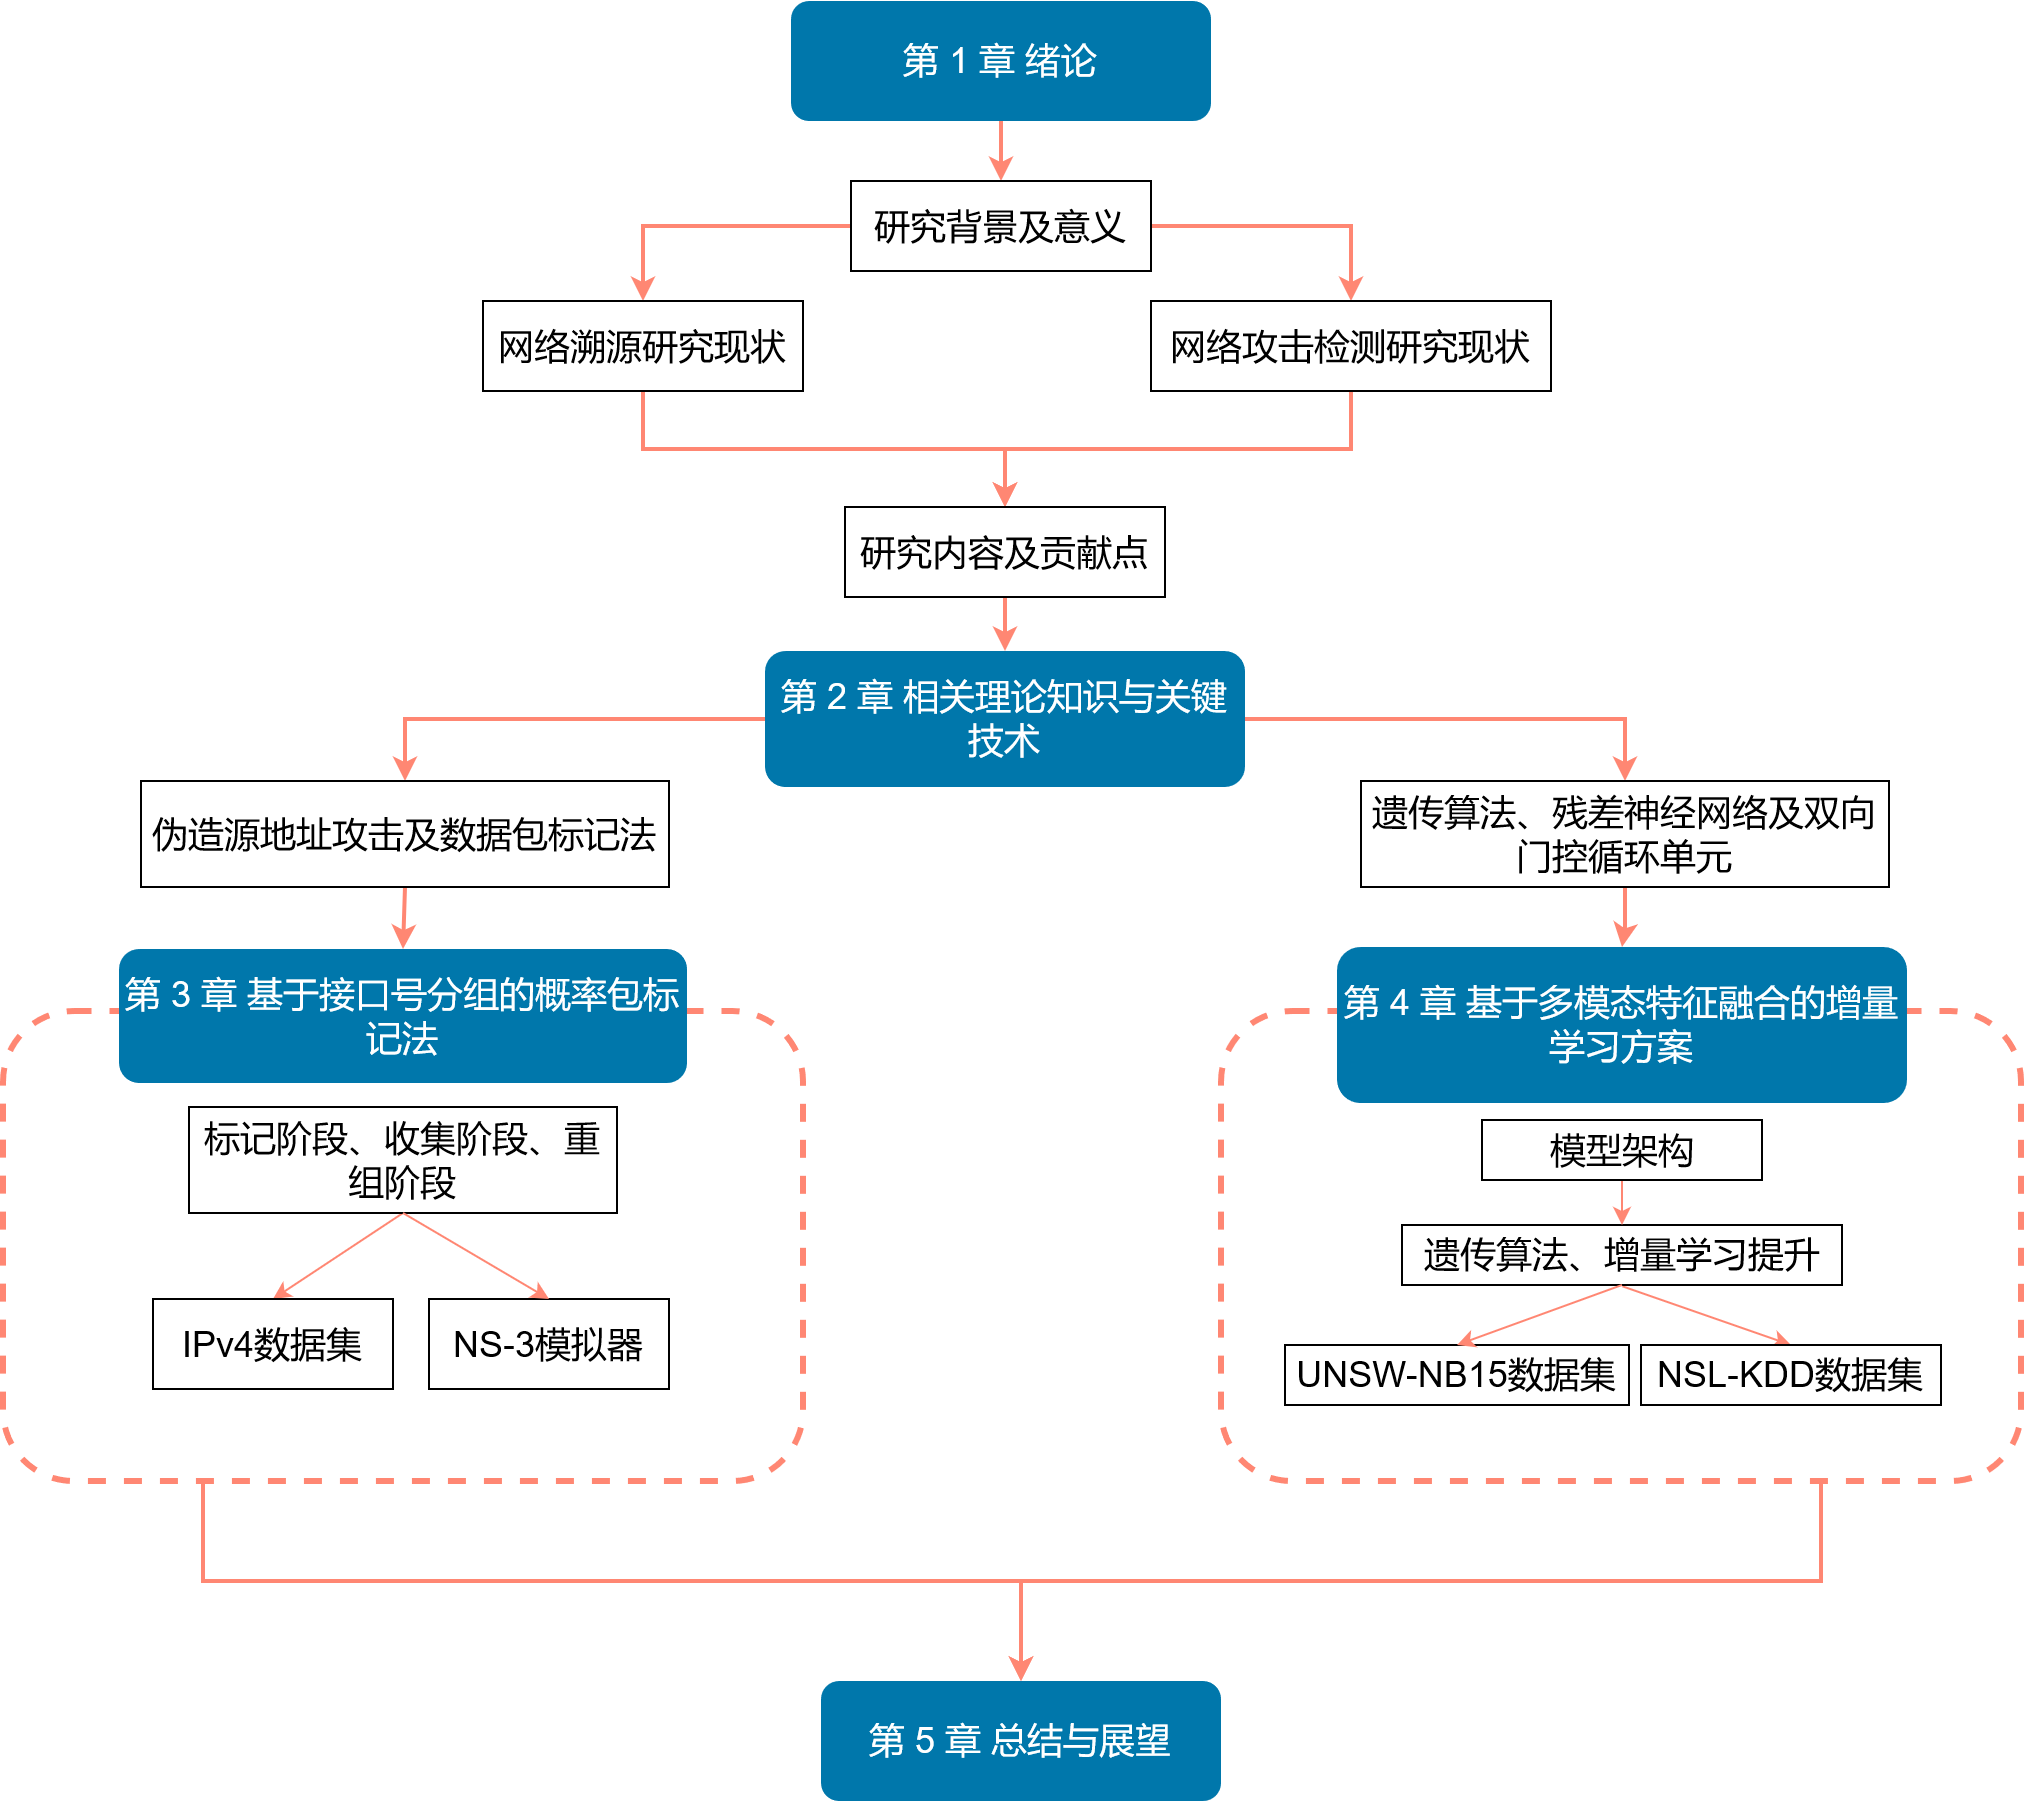
\includegraphics[width = 0.8\textwidth]{paper_structure.drawio.png}
  \caption{论文组织结构}
  \label{fig:paper_structure}
\end{figure}

第~\ref{cha:overview}~章,绪论。
在本章主要介绍了我们的研究,即基于特征融合的异常流量检测模型及防护方法研究,所处的背景以及具备的研究意义。
之后,本文详细地介绍了网络溯源技术的研究现状。
最后交代了本文的研究内容及主要贡献点以及论文的组织架构。


第~\ref{cha:basic-knowledge}~章概述了残差神经网络、双向门控循环单元网络、遗传算法、伪造源地址攻击与数据包标记法的相关理论基础。

% 第~\ref{cha:ResNet-BiGRU}~章, 基于特征融合的异常流量检测模型与增量学习实现。
% 本文首先提出了一个基于残差网络与双向门控循环单元的多模态特征融合模型,并对其原理和结构进行了详细的介绍。
% 随后经过几组对比实验验证了该模型的优越性。
% 接着,本文又基于此模型结合iCaRL技术提出了一个多模态特征融合的增量学习方案。
% 为进一步优化该方案的性能,本文又提出了一个基于遗传算法的记忆集抽样优化策略。
% 最后利用UNSW-NB15和NSL-KDD数据集分别作为新旧任务数据集对该方案进行了验证,验证结果表明该方案能够有效支持模型的增量学习和知识保留。


第~\ref{cha:ResNet-BiGRU}~章首先提出了基于残差网络与双向门控循环单元的多模态特征融合模型,并通过实验验证了其优越性。
接着本文基于此模型结合iCaRL技术,实现了增量学习方案。
为进一步优化该方案的性能,本文又提出了一个基于遗传算法的记忆集抽样优化策略。
最后利用UNSW-NB15和NSL-KDD数据集分别作为新旧任务数据集对该方案进行了实验验证,实验证明该方案能有效支持模型增量学习和知识保留。

第~\ref{cha:IGPPM}~章,基于接口号分组的概率标记溯源防护方法。
本章首先提出了基于接口号分组的概率标记溯源防护方法,并介绍了该方法的原理及流程。
随后,本文通过几组对比实验,展示了该溯源方法在溯源准确率和溯源速度方面的性能表现。
最后,本文设计了该溯源方法对模型进行防护的具体原理和流程。

% 第~\ref{cha:IGPPM}~章提出了基于接口号分组的概率标记溯源防护方法,包括其运行的三个阶段。
% 通过对比实验,展示了该方法在溯源准确率和速度上的优势,最后详细设计了其对模型保护的原理和流程。


第~\ref{cha:over_view}章,总结和展望。
总结了本文的所有研究工作以及取得的成果,最后指出了本文未来的研究内容和方向。

最后是参考文献、攻读硕士学位期间发表的学术论文目录和致谢。

%%================================================
%% Filename: chap02.tex
%% Encoding: UTF-8
%% Author: Yuan Xiaoshuai - yxshuai@gmail.com
%% Created: 2012-04-27 19:37
%% Last modified: 2019-11-05 23:57
%%================================================
\chapter{相关理论知识与关键技术}
\label{cha:basic-knowledge}

% \section{深度学习}
% 深度学习是机器学习的一个子集,它的算法受到人脑中的神经网络结构的启发,用于帮助机器识别模式和数据中的特征。
% 这种识别是通过一个多层次的抽象层完成的,每一层都会对信息进行加工和提炼,从而让机器能够理解复杂的数据,执行分类、识别等任务。

% 深度学习的核心构成是深度神经网络,这些网络除了包含输入层和输出层外,还嵌入了多个隐藏层,这种多层的叠加构造出了复杂且深远的网络结构。
% 图~\ref{fig:nerualnetwork}~展示了一个简单的神经网络结构。
% 在这一结构中,每一层都可以由众多节点或神经元组成,这些节点通过权重相互连接。
% 这些权重在训练过程中通过反向传播算法进行调整,以最小化预测和实际结果之间的差异。
% 这样的设计使得深度神经网络能够处理和学习大量复杂数据,从而在多种任务和应用中实现高度精确的预测和识别。

% \begin{figure}[htbp]
%   \centering
%   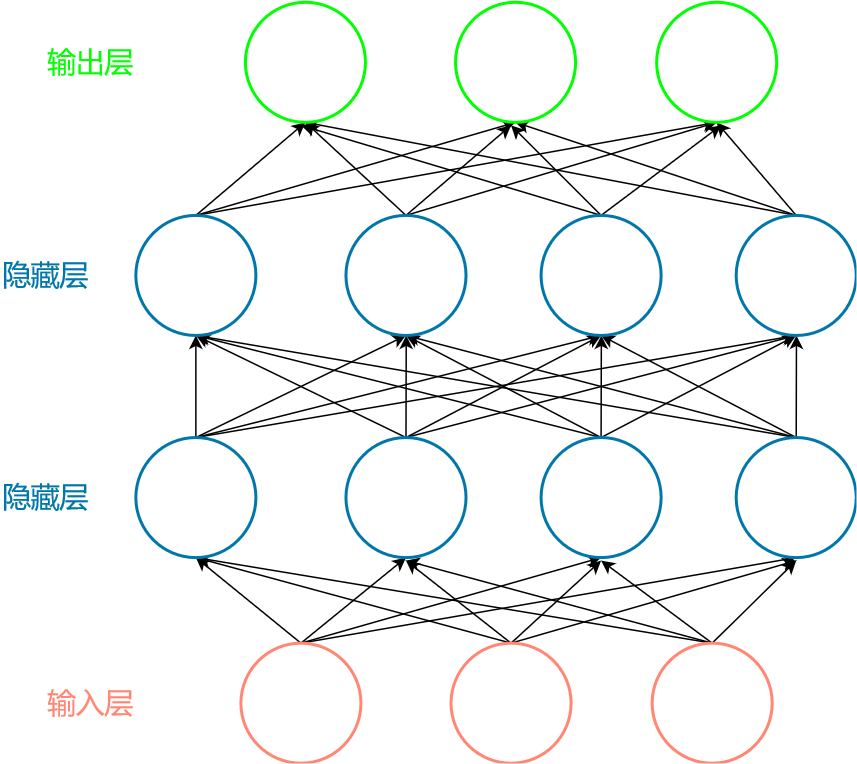
\includegraphics[width = 0.6\textwidth]{nerualnetwork.drawio.png}
%   \caption{神经网络结构图}
%   \label{fig:nerualnetwork}
% \end{figure}

\section{残差神经网络}
残差神经网络(Residual Neural Network,简称ResNet)是一种深度神经网络架构,它在2015年被提出,并且因其出色的性能获得了ImageNet大规模视觉识别挑战(ILSVRC)\footnote{http://image-net.org/challenges/LSVRC/2015/ 和 http://mscoco.org/dataset/\#detections-challenge2015.}的胜利\cite{he2016deep}。
ResNet的提出,解决了深度网络训练过程中的梯度消失以及梯度爆炸问题,使得训练更深层次的网络模型成为可能,从而极大地提高了图像识别、分类任务的准确率。

在传统的深度神经网络中,随着网络层数的加深,训练难度逐渐增大。
这主要是因为梯度在反向传播过程中会逐渐消失或爆炸,导致网络权重难以得到有效更新。
为了解决这个问题,ResNet引入了“残差学习”的概念,即通过添加跳跃连接(Shortcut Connections)将输入信息直接传递到更深层的网络中,为信息流动提供了一条更短的路径。

ResNet由多个残差块组成,每个残差块内部包含多层卷积层和一个跳跃连接(图~\ref{fig:resnet_structure}展示了一个由两层卷积层堆叠而成的残差块结构)。
\begin{figure}[h]
  \centering
  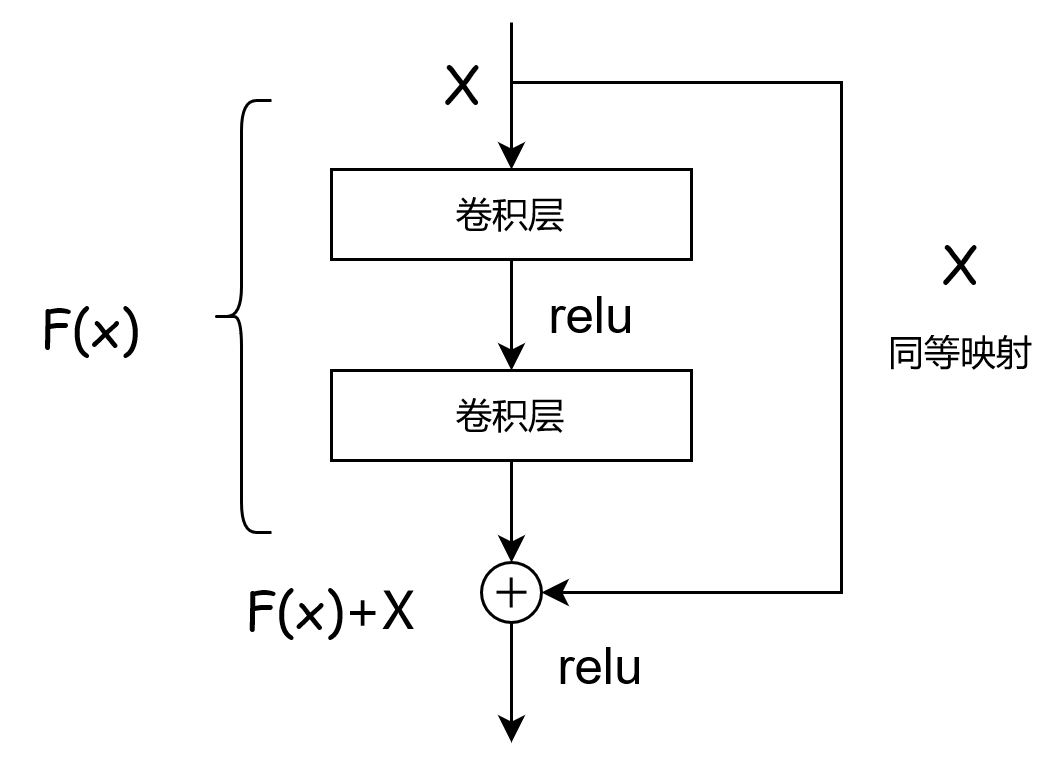
\includegraphics[width = 0.6\textwidth]{resnet_block.drawio.png}
  \caption{两层堆叠的残差块结构图}
  \label{fig:resnet_structure}
\end{figure}
通过跳跃连接,ResNet能有效地解决梯度消失和爆炸问题,使得训练深度模型成为可能。


跳跃连接的原理在于,ResNet不再要求网络层直接拟合一个期望的底层映射,而是让网络层拟合一个残差映射。
假设期望的底层映射为H(x),那么网络层需要拟合的残差映射则为:
\begin{equation}
  \label{eq:residual_mapping}
  F(x) := H(x) - x
\end{equation}
因此,原始映射可以重新表述为F(x)+x。
这种优化方式使得网络更容易学习到恒等映射,从而确保增加的层不会降低网络的性能。
通过这种方法,我们便可以构建更深的网络模型而不会降低性能,这在许多图像视觉识别任务中都实现了前所未有的准确率。


此外,ResNet的应用范围不仅局限于图像分类、检测和识别任务。
其强大的特征提取能力和优秀的性能表现使得它在自然语言处理、音频分析等其他领域也得到了广泛的应用。
可以说,ResNet的提出为深度学习领域的发展注入了新的活力。

% 卷积神经网络\cite{lecun1998gradient}(Convolutional Neural Networks, CNNs)是一种专门用于处理具有类似网格结构数据的深度学习算法,最典型的应用是图像处理,其中数据可以被视为2D网格。
% CNNs的设计灵感来源于生物的视觉皮层结构,特别是视觉皮层中那些负责处理光线、阴影、边缘等视觉元素的神经元的组织方式。

% 卷积神经网络的关键特性之一是其能够自动、有效地学习空间层次的特征。
% 这是通过网络中的卷积层来实现的,它们使用一组可学习的滤波器或卷积核扫描整个图像或信号。
% 这些滤波器能够捕捉到局部依赖性(例如边缘或纹理)和图像中的空间层次结构,使得CNN非常适合处理图像和视频数据。

% CNN通常包含三种类型的层:卷积层、池化层和全连接层。
% 图~\ref{fig:cnnnetwork}~展示了一个简单的卷积神经网络结构。
% 卷积层负责提取图像中的特征;
% 池化层用于减少数据的空间大小,提高计算效率,同时保持重要的特征;
% 全连接层则用于将网络中的特征汇总,并进行最终的分类或回归分析。

% \begin{figure}[htbp]
%   \centering
%   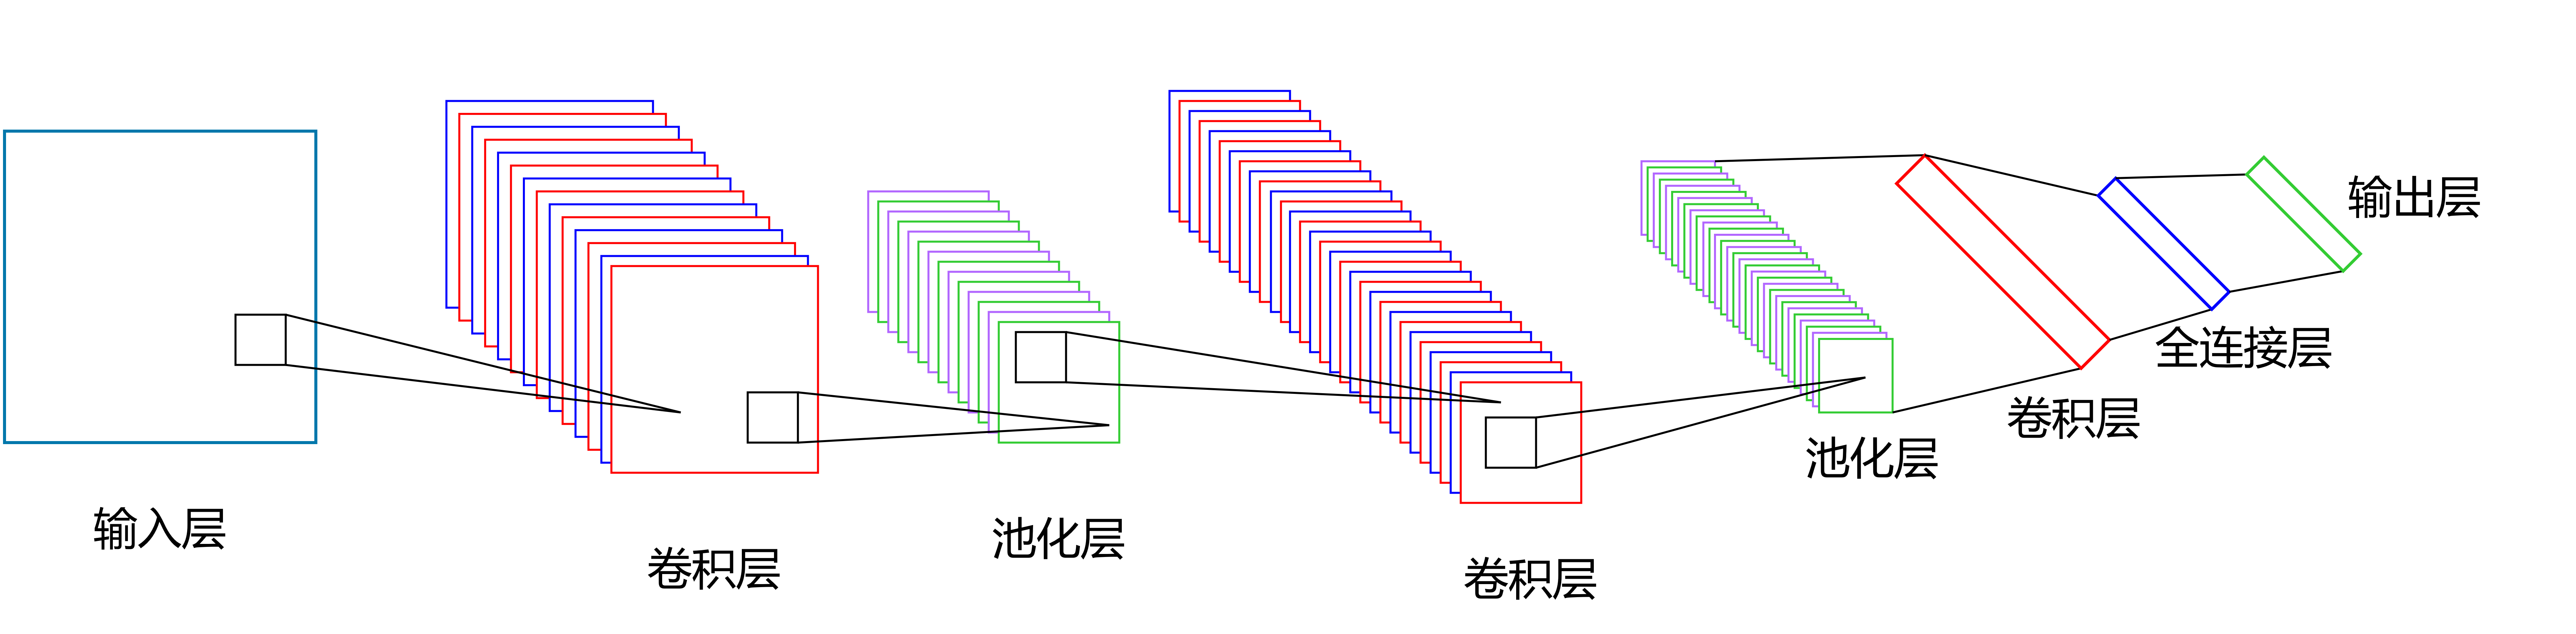
\includegraphics[width = 1.0\textwidth]{cnnstructure.drawio.png}
%   \caption{卷积神经网络结构图}
%   \label{fig:cnnnetwork}
% \end{figure}

% \subsubsection*{残差神经网络}
% 残差神经网络(Residual Neural Network,简称ResNet)是一种深度神经网络架构,它在2015年被提出,并且因其出色的性能获得了ImageNet大规模视觉识别挑战(ILSVRC)\footnote{http://image-net.org/challenges/LSVRC/2015/ 和 http://mscoco.org/dataset/\#detections-challenge2015.}的胜利\cite{he2016deep}。
% ResNet的核心思想是引入了“残差学习”的概念,以解决深度网络训练过程中的梯度消失或梯度爆炸问题,这使得我们能够成功地训练出比以往更深的网络模型,极大地提高了识别和分类任务的准确率。


% % 如图~\ref{fig:traintesterror}~所示,
% 在传统的深度神经网络中,随着层数的增加,网络变得越来越难以训练,这主要是因为梯度在反向传播时会逐渐消失或爆炸,导致网络权重难以更新\cite{he2016deep}。


% % \begin{figure}[h]
% %   \centering
% %   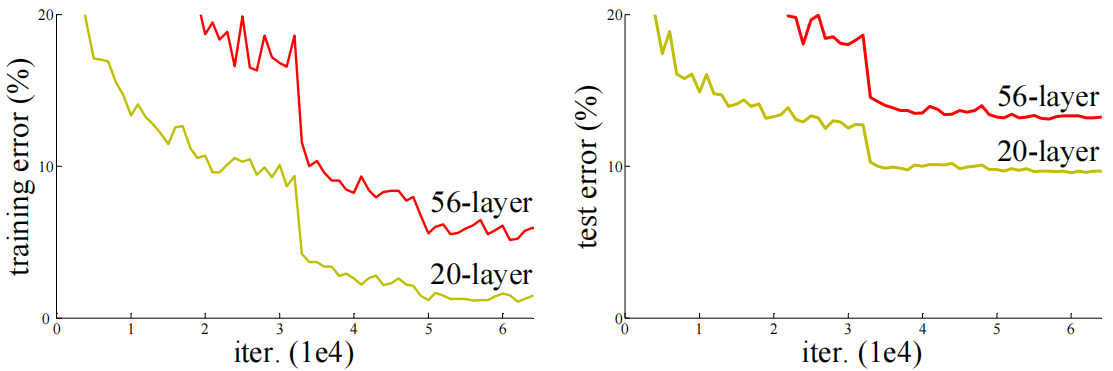
\includegraphics[width = 0.8\textwidth]{traintesterror.png}
% %   \caption{20层和56层的“普通”网络在CIFAR-10数据集上训练结果,左图是训练误差,右图是测试误差\cite{he2016deep}。}
% %   \label{fig:traintesterror}
% % \end{figure}

% 残差网络通过添加直接的跳跃连接(Shortcut Connections)来解决这个问题。
% 这些跳跃连接允许输入直接传递到后面几层中,从而在不同层之间创建了一条更短的路径。
% % 跳跃连接(Shortcut Connections)是ResNet的标志性设计,它们使得输入可以跳过一层或多层直接传递到更深的层。
% 在实践中,这意味着深层网络能够学习到一个恒等映射,确保增加的层可以至少不会降低网络的性能。
% 这背后的原理是不再利用多层堆叠的块直接拟合一个期望的底层映射,而是明确让这个块拟合一个残差映射。
% 形式上,假设期望的底层映射为$H(x)$,而我们让堆叠的块拟合另一个映射,即残差映射:
% \begin{equation}
%   \label{eq:residual_mapping}
%   F(x) := H(x) - x
% \end{equation}
% 因此原始映射将被重新表述为$F(x) + x$。
% 这样做的好处是,优化残差映射比优化原始的、未引用的映射更容易。
% % 图~\ref{fig:Resnetvsplai}~是18层、34层普通网络与残差网络在ImageNet数据集上训练误差与测试误差对比结果。
% % \begin{figure}[htbp]
% %   \centering
% %   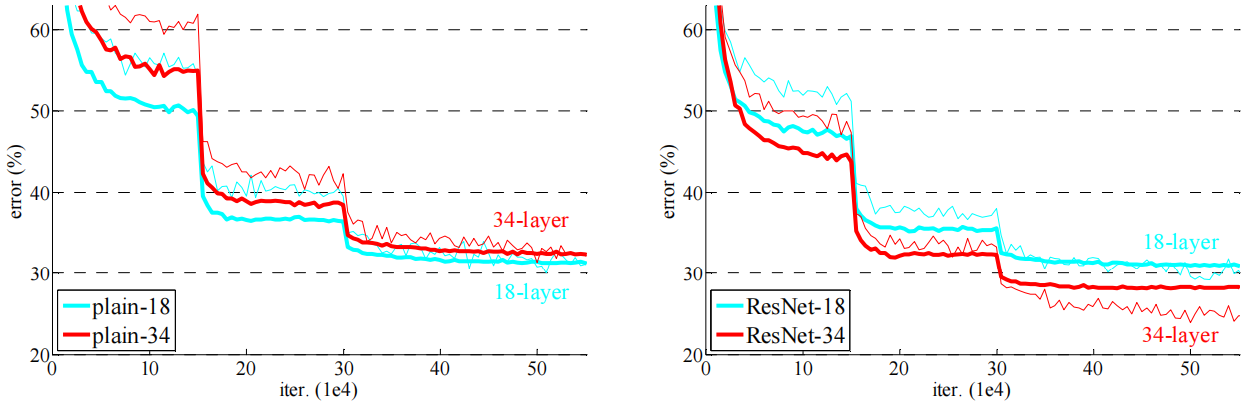
\includegraphics[width = 0.8\textwidth]{Resnetvsplain.png}
% %   \caption{18层、34层“普通”网络与残差网络在ImageNet数据集上训练误差与测试误差对比结果\cite{he2016deep}。}
% %   \label{fig:Resnetvsplai}
% % \end{figure}
% % 可以看到
% 残差网络相比层数相同的普通网络具有更好的训练效果以及更快的优化速度。



% 残差网络由多个残差块组成,每个块内部都有几层卷积层和一个跳跃连接。
% 图~\ref{fig:resnet_structure}~展示了一个由两层权重层堆叠的残差块。
% \begin{figure}[htbp]
%   \centering
%   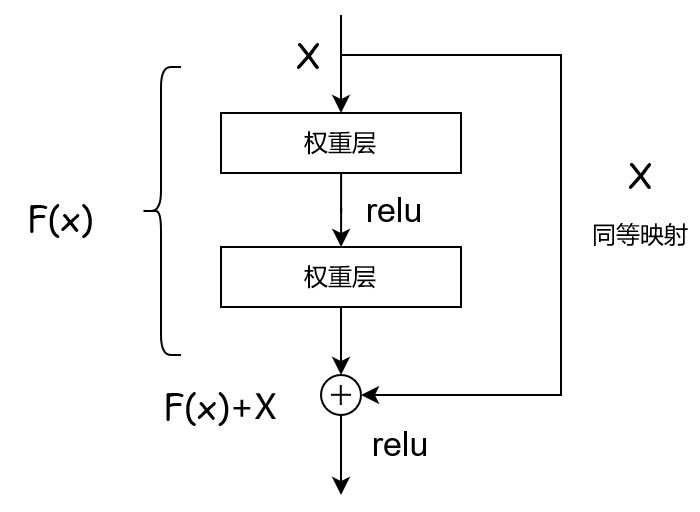
\includegraphics[width = 0.6\textwidth]{ResNet.drawio.png}
%   \caption{两层堆叠的残差块结构图}
%   \label{fig:resnet_structure}
% \end{figure}
% 通过跳跃连接,ResNet解决了梯度消失和爆炸问题,使得训练深度模型成为可能。
% ResNet允许我们构建更深的网络模型而不会降低性能,这在许多视觉识别任务中都实现了前所未有的准确率。
% ResNet不仅在图像分类、检测和识别任务中表现出色,也被广泛应用于其他领域,如自然语言处理和音频分析。

% \section{循环神经网络}
% 由于传统的神经网络主要由独立运作的输入层、隐藏层以及输出层构成,所以数据仅能在这些层间单向传递,这限制了其处理时间序列数据的能力。
% 对于那些数据内容随时间变化而紧密相关的场景,如视频、音频及文本等,传统神经网络难以有效捕捉其中的时序特征。
% 因此,为了克服这一限制并优化对时序数据的处理,研究者们提出了循环神经网络(Recurrent Neural Network,RNN)\onlinecite{lecun2015deep}。


% RNN是一种专为处理序列数据而设计的神经网络架构。
% 与传统的前馈神经网络不同,RNN能够处理输入数据之间的时间动态性,使其特别适用于语言模型、语音识别、机器翻译等领域。
% RNN的基本单元包括输入层、一个或多个循环隐藏层以及输出层。
% RNN的基本单元结构如图~\ref{fig:RNNunit}~所示。
% \begin{figure}[htbp] 
%   \centering
%   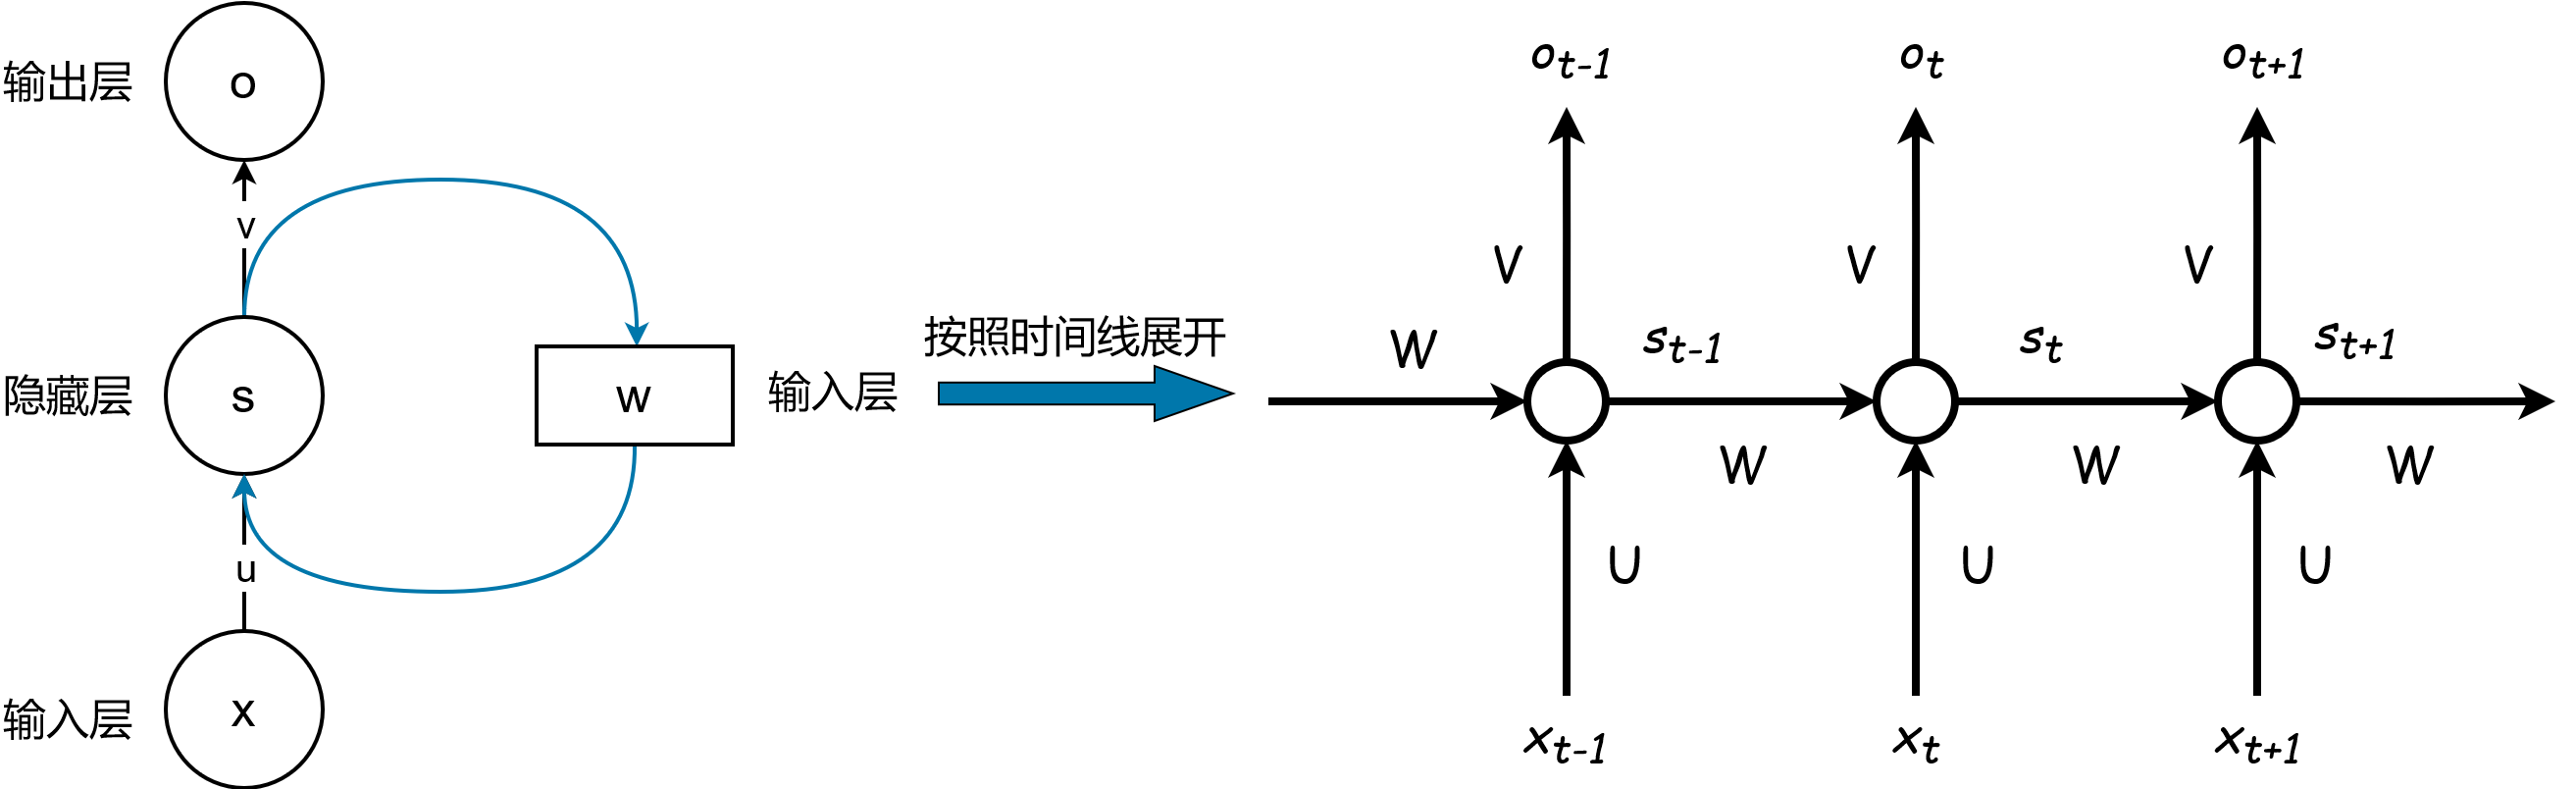
\includegraphics[width = 1.0\textwidth]{RNNunit.drawio.png}
%   \caption{RNN基本单元结构图}
%   \label{fig:RNNunit}
% \end{figure}


% 由于RNN的网络结构设计允许在处理序列数据时,将前一时间步的信息传递到当前时间步,这使得RNN具备短期记忆能力。
% 这种能力主要通过网络中的隐藏层状态实现,其中每个时间步的隐藏状态都依赖于前一个时间步的隐藏状态和当前时间步的输入。
% 具体来说,RNN的每个时间步都会接收两个输入:当前时间步的数据输入和前一时间步的隐藏层状态。
% 例如,在 t 时刻,输入层将$x_t$输入到隐藏层$s_t$的同时,隐藏层的上一个输出$s_{t-1}$也作为输入,输入到隐藏层$s_t$中。
% 由此,t 时刻的输出和隐藏层的值计算方式如公式~\ref{eq:RNN_ot}、\ref{eq:RNN_st}~所示:
% \begin{gather}
%   O_t = g(V \cdot S_t) \label{eq:RNN_ot} \\
%   S_t = f(U \cdot X_t + W \cdot S_{t-1}) \label{eq:RNN_st}
% \end{gather}
% \begin{flushleft}
%   \renewcommand\arraystretch{1.25}
%   \begin{tabularx}{\textwidth}{@{}>{\normalsize\rm}l@{\quad}>{\normalsize\rm}l@{——}>{\normalsize\rm}X@{}}
%   式中
%   &  $g$ &输出层神经元激活函数;\\
%   &  $f$ &隐藏层神经元激活函数;\\
%   &  $V$   &隐藏层到输出层权重参数;\\
%   &  $U$ & 输入层到隐藏层权重参数;\\
%   &  $W$ & t-1时刻隐藏层输出到t时刻隐藏层输出权重参数;\\
%   &  $x_t$ &t时刻输入;\\
%   &  $s_t$ & t时刻隐藏层输出;\\
%   \end{tabularx}\vspace{.5ex}%TODO : 注释内容自动转页接排
% \end{flushleft}

% 这个隐藏层状态包含了之前时间步的信息,相当于网络的“记忆”。
% 然后,RNN通过当前的输入和这份“记忆”来更新其隐藏状态,以及生成当前时间步的输出。
% 通过这种机制,RNN能够在处理每个时间步的数据时,考虑到序列之前的信息,实现对信息的短期记忆。

\section{双向门控循环单元}
传统的循环神经网络(RNN)在处理长序列数据时,往往会遭遇梯度消失和梯度爆炸的挑战。
梯度消失导致网络难以捕获长期依赖关系,因为随着序列长度的延伸,早期时间步的信息对后续时间步的影响逐渐减弱,仿佛被“遗忘”。
而梯度爆炸则可能引发训练过程的不稳定,使得模型难以收敛。
为了克服这些限制,研究者们提出了更为先进的循环网络结构,如长短期记忆网络(LSTM)\cite{memory2010long}和门控循环单元(GRU)\cite{cho2014learning}。
这些结构通过精心的设计,显著增强了网络对长期依赖关系的捕捉能力。
% 虽然RNN理论上能够捕捉序列中的长距离依赖关系,但在实践中,由于梯度消失或梯度爆炸的问题,其实际的记忆能力往往被限制在较短的序列上。
% 所以后来的研究者门提出了如长短期记忆网络(LSTM)\cite{memory2010long}和门控循环单元(GRU)\cite{cho2014learning}等更高级的循环网络结构,它们通过特殊的设计来显著提高网络对长期依赖关系的捕捉能力。
LSTM 通过门控机制使循环神经网络不仅能记忆过去的信息,同时还能选择性地忘记一些不重要的信息而对长期语境等关系进行建模,而 GRU 基于这样的想法在保留长期序列信息下减少梯度消失问题。
相比LSTM,使用GRU能够达到相当的效果,并且相比之下更容易进行训练,能够很大程度上提高训练效率,因此很多时候会更倾向于使用GRU。

图~\ref{fig:GRUunit}~是GRU基本单元的组成结构图。
\begin{figure}[h] 
  \centering
  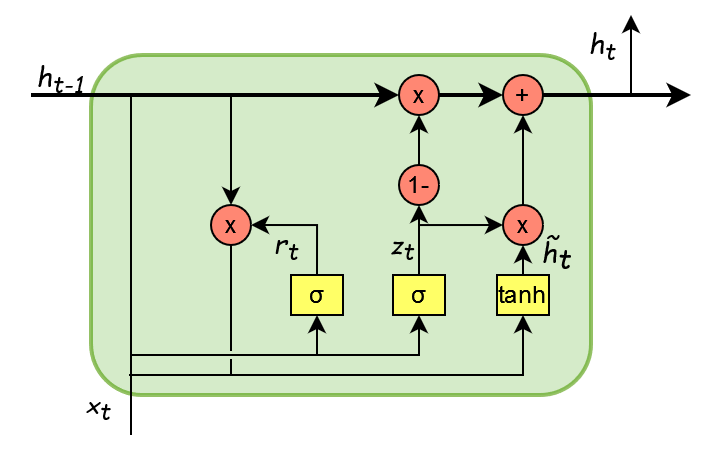
\includegraphics[width = 0.8\textwidth]{gru.drawio.png}
  \caption{GRU基本单元结构图}
  \label{fig:GRUunit}
\end{figure}
\begin{flushleft}
  \renewcommand\arraystretch{1.25}
  \begin{tabularx}{\textwidth}{@{}>{\normalsize\rm}l@{\quad}>{\normalsize\rm}l@{——}>{\normalsize\rm}X@{}}
  图~\ref{fig:GRUunit}~中
  &  $\times$ &Hadamard Product,矩阵相乘运算;\\
  &  $+$ &矩阵加法运算;\\
  &  $σ$ &Sigmoid 激活函数,输出范围为0 -- 1;\\
  &  $\tanh$ & $\tanh$激活函数,输出范围为-1 -- 1;\\
  \end{tabularx}\vspace{.5ex}%TODO : 注释内容自动转页接排
\end{flushleft}

GRU由重置门(reset gate)和更新门(update gate)两种类型的门控机制构成。
这些门控制着信息的流动,决定了哪些信息应当被保留,哪些信息应当被忽略或删除,从而有效地捕捉到长期依赖性。

其中,重置门决定了多少过去的信息需要被忘记。
它允许模型抛弃与新信息无关的旧状态信息,使模型能够更灵活地处理每个时间点的数据。
GRU得到门控信号$r_t$之后,首先使用重置门控来得到“重置”之后的数据$h'_{t-1} = r_t \cdot h_{t-1}$,再将$h'_{t-1}$与输入$x_t$进行拼接,再通过一个$\tanh$激活函数来将数据放缩到-1 -- 1的范围内。
这一过程如公式~\ref{eq:gru_rt}、\ref{eq:gru_ht}~所述。
\begin{gather}
  r_t = σ(W_r \odot [h_{t-1},x_t]) \label{eq:gru_rt} \\
  \tilde{h_t} = \tanh(W \odot [r_t \cdot h_{t-1} , x_t]) \label{eq:gru_ht}
\end{gather}
这里的$h'_{t-1}$主要是包含了当前输入的$x_t$数据。
有针对性地对$h'_{t-1}$添加到当前的隐藏状态,相当于“记忆了当前时刻的状态”。
类似于LSTM的选择记忆阶段。


更新门帮助模型决定过去的信息有多少需要保留到未来。
它在决定状态信息是否更新时起着关键作用,类似于LSTM中的遗忘门和输入门的组合。
“更新记忆”阶段是GRU最关键的一个阶段。
在这个阶段,GRU同时进行了遗忘与记忆两个步骤。
我们使用了先前得到的更新门控$z$得到更新表达式: 
\begin{equation}
  \label{dq:gru_ht}
  h_t = (1-z) \odot h_{t-1} + z \odot h'_{t-1}
\end{equation}
门控信号$z$的范围为0 -- 1。门控信号越接近1,代表“记忆”下来的数据越多;而越接近0则代表“遗忘”的越多。
可以看到,这里的遗忘$z$和选择$(1-z)$是联动的。
也就是说,对于传递进来的维度信息,我们会进行选择性遗忘,则遗忘了多少权重($z$),GRU就会使用包含当前输入的$h'_{t-1}$中所对应的权重进行弥补。
以保持一种“恒定”状态。

% \subsubsection*{双向门控循环单元}

尽管GRU能够有效地处理序列数据中的长期依赖关系,并通过门控机制来控制信息的流动,但它在某些任务中仍然存在一些挑战。
具体而言,GRU只能按照序列的时间顺序依次处理每个时间步的信息,这意味着在处理某个时间步时,它只能利用该时间步之前的信息,而无法同时利用该时间步之后的信息。
然而,在某些任务中,我们需要同时考虑序列中过去和未来的信息。
例如,在语音识别或自然语言处理中,当前词的识别或理解可能不仅取决于它之前的词,还取决于它之后的词。
在这种情况下,单向的GRU可能无法充分捕获序列中的上下文信息。
为了解决这个问题,我们可以引入双向门控循环单元(Bi-directional GRU,BiGRU)。
与单向的GRU不同,双向GRU在每个时间步都会同时考虑正向和反向的序列信息。
具体来说,它会分别从前向和后向两个方向对序列进行处理,然后将两个方向上的隐状态进行拼接或求和等操作,以得到每个时间步的最终输出。
% 双向门控循环单元(Bidirectional Gated Recurrent Unit, BiGRU)是一种特殊类型的循环神经网络(RNN)结构,它结合了GRU(门控循环单元)的优势和双向RNN的特点,以更有效地处理序列数据。
% BiGRU通过同时处理过去和未来的信息,能够在序列处理任务中,如自然语言处理(NLP)和语音识别,提供更丰富的上下文信息。
% BiGRU除了具备GRU的门控机制之外另一个核心特点是核心特点是双向处理。
图~\ref{fig:GRUunit}~展示的是一个沿着时间展开的双向循环神经网络。
\begin{figure}[h]
  \centering
  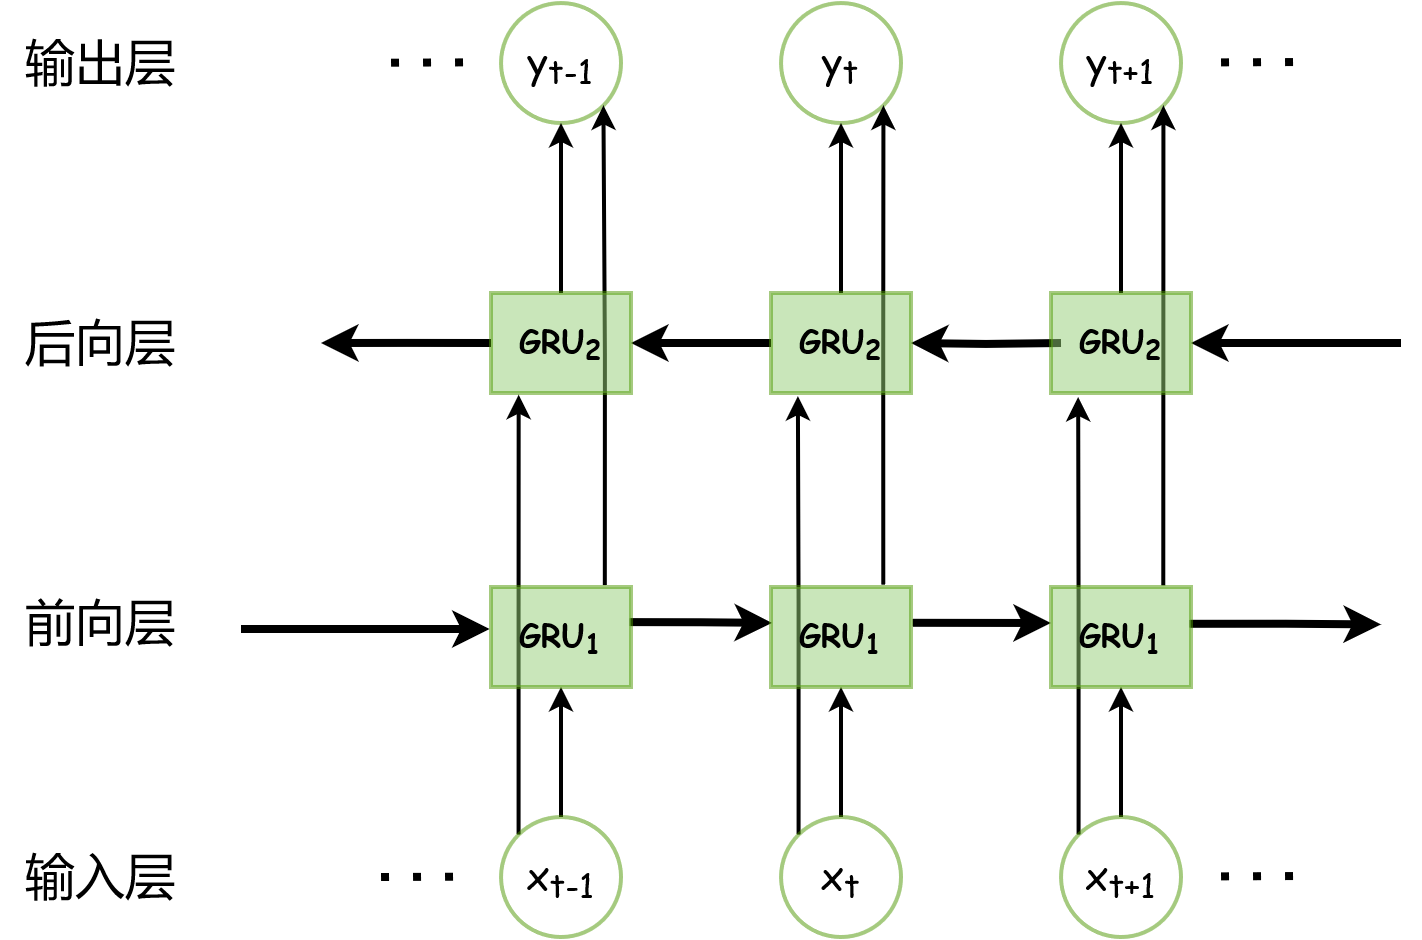
\includegraphics[width = 0.6\textwidth]{BiGRU.drawio.png}
  \caption{BiGRU结构图}
  \label{fig:BiGRU}
\end{figure}

BiGRU包含两个GRU层,一个沿正时间方向处理数据(正向GRU),捕捉从过去到现在的依赖;
另一个沿反时间方向处理数据(反向GRU),捕捉从未来到现在的依赖。
这两个层的输出通常会在每个时间步被合并,以提供给定时间点前后的完整上下文信息。
另外,从GRU继承的更新门和重置门可以使模型在每个方向上更有效地学习长期和短期依赖性。

对于一个输入序列 $X = x_1 x_2 \dots x_T$,BiGRU模型的前向计算可以表示为:
\begin{gather}
  \overleftarrow{h_t} = GRU_1(x_t,\overleftarrow{h_{t-1}}) \label{eq:bigru_htleft} \\
  \overrightarrow{h_t} = GRU_1(x_t,\overrightarrow{h_{t-1}}) \label{eq:bigru_htright} \\
  y_t = \overleftarrow{h_t} \oplus \overrightarrow{h_t} \label{eq:bigru_out}
\end{gather}
\begin{flushleft}
  \renewcommand\arraystretch{1.25}
  \begin{tabularx}{\textwidth}{@{}>{\normalsize\rm}l@{\quad}>{\normalsize\rm}l@{——}>{\normalsize\rm}X@{}}
  其中
  &  $y_t$ &模型输出;\\
  &  $\overrightarrow{h_t}$ &前向输出;\\
  &  $\overleftarrow{h_t} $ &后向输出;\\
  &  $\oplus$ & element-wise sum按位加。\\
  \end{tabularx}\vspace{.5ex}%TODO : 注释内容自动转页接排
\end{flushleft}

\section{源地址伪造攻击的分类}

源地址伪造攻击可以根据伪造产生的虚假地址与攻击者受害者所在网络的关系来进行分类,总共可分为六类:
a.虚假地址在网络中不存在或已经失活;
b.虚假地址指向的主机是受害者;
c.虚假地址与受害者主机处于同一个子网中;
d.虚假地址与攻击者处于同一个子网中;
e.虚假地址处于攻击者和受害者之间的路径中;
f.虚假地址既不在攻击者与受害者的子网中也不在攻击者与受害者之间的路径当中\cite{Bi2010}。
以下是这六类攻击的详细描述。

1)~a类\par
恶意主机通过产生随机的互联网中不存在的或着已经失效的IP地址来对攻击数据包的源地址进行伪造。
产生的攻击数据包占用着受害者主机的资源,使受害者不能再向其他主机提供服务。
这些IP地址包括RFC1918中指定的私有IP地址\cite{Rekhter1996}、RFC3330中的自动分配的IP地址\cite{BogonList2003}、循环测试地址,它们均不会在互联网中出现。
SYN Flood是一种常见的攻击方式,它能够不断消耗受害者主机CPU资源以及内存资源并阻止其他合法用户的连接。
在不设置保护策略的情况下,少量的SYN洪水攻击便足以使受害者主机崩溃。
由于受害者主机在受到攻击时会向恶意数据包中源地址指向的主机返回SYNACK包使其返回RTS包释放半连接。
这就导致了此种攻击将会采用上面所说的地址来对攻击数据包的源地址进行伪造。\par
2)~b类\par
攻击者将受害者主机的IP地址作为攻击数据包的源地址以此来实现反射性攻击、直接攻击和诱捕攻击,这类攻击通常有三种形式:
第一种形式,攻击数据包的源地址是受害者主机IP地址,目标地址是受害者主机的所在子网的广播地址。
攻击数据包被广播之后,受害者将收到大量的ACK回复,这会使受害者淹没于这些流量当中而大大地削弱了受害者的正常服务能力。
第二种形式,攻击数据包的源地址与目标地址同时是受害者主机的IP,受害者收到攻击数据包后会将其响应发送给自己,这一行为会导致受害者受到干扰而瘫痪。
著名的DrDoS\cite{Gibson2002}是此类攻击的一个典型例子,它会使受害者的带宽或内存等资源溢出或者过载而不能使用。
TFN\cite{Dittrich1999}和Land  attacks\cite{CERT1997}也是此类典型的例子。
第三种形式,攻击者向受害者发送数据包,其源主机/端口与目标主机/端口相同,并设置了SYN标志能够锁死受害者或使其协议栈崩溃。\par
3)~c类\par
此类攻击将受害者子网内的IP地址伪装成攻击数据包的源地址,借助受害者与伪造地址对应主机间的信任关系实施攻击。
基于TCP连接的盲IP欺骗攻击\cite{Ali2007}是这类攻击的典型例子。
TFN2K\cite{Barlow2000}也是一个例子,它是TFN\cite{Dittrich1999}的下一代版本。\par
4)~d类\par
d类攻击将攻击者所处子网内的地址作为源地址,因为入口过滤的粒度通常不高便可以很容易使攻击数据包通过入口过滤。
反弹扫描\cite{CERT1997}是这类攻击的典型案例。攻击者通过伪造同一子网内邻居的源地址,诱使受害者发送响应包,进而嗅探并截获返回给邻居的流量数据。
此类攻击可用于端口扫描,当受害者的某端口处于关闭状态时,会回复RST数据包\cite{Ray1981}。更为严重的是,这种攻击能巧妙地规避uRPF的防御机制\cite{CiscoIOS2005},从而增加了网络安全的隐患。\par
5)~e类\par
e类攻击的攻击者通常强迫网络设备的源地址出现在攻击者与受害者之间的路径上。
在此过程中,攻击者能散布虚假的DNS或路由信息,并实现对网络流量的重定向\cite{Huang2006}。此类攻击因其高度的隐蔽性和破坏力,被视为极具危险性的网络攻击手段之一。\par
6)~f类\par
此类攻击无需依赖受害者与伪造地址间的特定拓扑关系。
攻击者常将多种攻击手段组合运用,如MITM攻击\cite{ManInTheMiddle2007},便是f类攻击中两种典型手法的结合。
以A、V1和V2为例,A在与V2通信时,会伪造V1的源地址;同样,在与V1通信时,A会伪造V2的源地址,从而实施攻击。\par

表~\ref{tab:source_address_spoofing}~展示了这六种攻击之间的关系。
\begin{table}[htbp]
  \caption{源地址伪造攻击分类}
  \label{tab:source_address_spoofing}
  \centering
  \begin{tabular}{cccc}
  \toprule
  {\heiti 分类} & {\heiti 虚假地址状态} & {\heiti 与攻击者关系} & {\heiti 与受害者关系}  \\ 
  \midrule
  a类 & 不存在或已经失活 & 无 & 无 \\ 
  b类 & 存在 & 无 & 指向 \\ 
  c类 & 存在 & 无 & 同子网 \\ 
  d类 & 存在 & 同子网 & 无 \\ 
  e类 & 存在 & 攻击者到受害路径内 & 攻击者到受害者路径内 \\ 
  f类 & 不存在 & 无 & 无 \\ 
  \bottomrule
  \end{tabular}
\end{table}

\section{数据包标记法}
图~\ref{fig:simple_topology}~是一个IP回溯问题的简单网络拓扑图。
\begin{figure}[htbp]
  \centering
  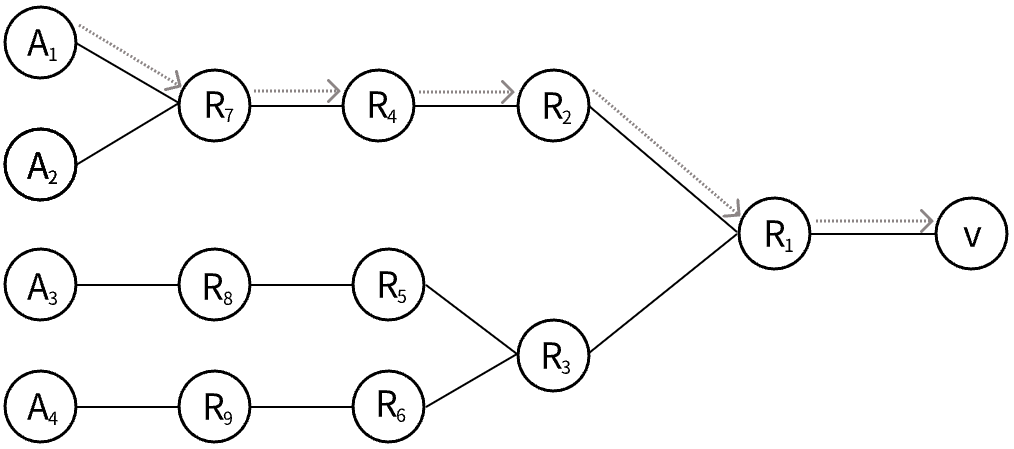
\includegraphics[width = 0.8\textwidth]{simple_topology.png}
  \caption{针对路由回溯问题的简单拓扑图}
  \label{fig:simple_topology}
\end{figure}
整个结构可以看作是一棵以$V$为根节点的树,$V$代表一个遭受攻击的受害者,它可能为服务器、防火墙或者入侵检测系统。
每个$A_i$是树中的叶子节点,它代表潜在的攻击源,它可能为例如攻击者主机也可能为普通的用户。
每个$R_i$则代表从这些$A_i$到$V$的中间路由器。
在这个网络中,每个$A_i$都有可能向$V$发送数据包,而这些数据包中则有潜在攻击数据包的可能性。
其中这些攻击数据包走过的路径都为攻击路径,它是一个从攻击节点$A_i$到$V$的有序唯一路由序列。
例如,假设$A_1$是一个攻击节点,它正在向$V$发送攻击数据包,这些攻击数据包走过的路径是唯一的,由$R_7$、$R_4$、$R_2$、$R_1$依次组成,则这条从$A_1$到$V$的唯一的路径就是一条攻击路径。
一个IP回溯问题就是通过一些方法和策略确定攻击路径,揭示攻击主机的真实身份和具体位置。



当回溯成功后便可以从攻击源的下游最近邻路由器过滤掉这些数据包以保护受害者服务器免受攻击。
在这个问题中,似乎只要从攻击数据包中提取出源IP就可以确定攻击路径,然而解决这个问题通常是很复杂的。
一个有预谋、有准备的攻击通常会做出一些手段,例如伪造攻击数据包的源IP地址、发送一些虚假信息来伪造攻击路径从而干扰溯源,使溯源任务极难完成。



% 一个IP回溯问题相对简单的近似溯源为找到一条包含有真实攻击路径作为路径后缀的候选路径,这个路径后缀就是有效后缀\cite{savage2000practical}。
% 例如,$R_8$、$R_5$、$R_3$、$R_7$、$R_4$、$R_2$、$R_1$就是一条有效的候选路径,因为它包含$R_7$、$R_4$、$R_2$、$R_1$这条真实的攻击路径作为候选路径的后缀。
% 而在接下来的本方案描述中却可以确定真实的攻击路径而不仅仅是候选路径,这是本方案的一大优势,这往往往需要网络中间设备来协作配合。



数据包标记法通常由两部分组成,即标记过程和路径重组过程。
当部署了本方案的路由器$R_i$接收到数据包后,便会执行标记过程。
在标记过程中,路由器$R_i$通过向待转发的数据包注入额外的标记信息来记录自身路由信息。
这些标记信息类型可能为路由器IP地址也可能是其他一些控制信息类型,具体的标记信息类型根据所选的方案而异。
通常,这些信息被注入到数据包的头部字段中,图~\ref{fig:ipv4_header}~显示了数据包头部字段被用作标记字段的情况。
\begin{figure}[htbp]
  \centering
  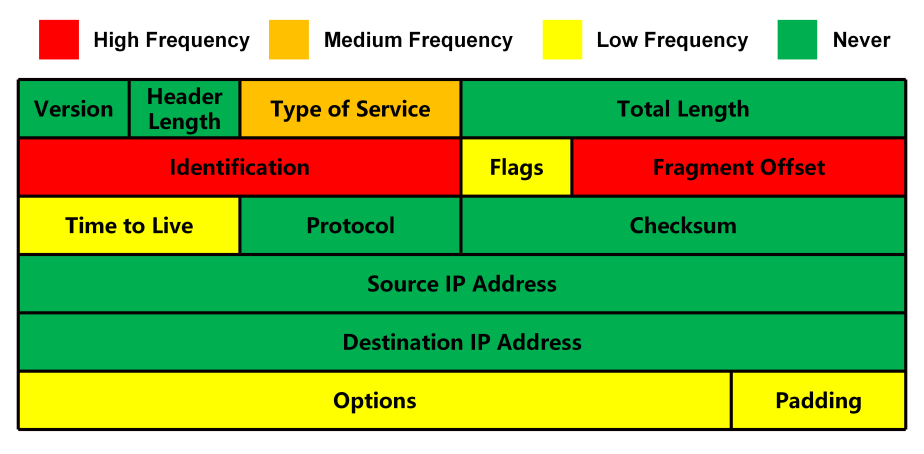
\includegraphics[width = 0.8\textwidth]{ipv4_header.png}
  \caption{标记过程中使用的IPv4头部字段}
  \label{fig:ipv4_header}
\end{figure}
当受害者$V$成功收集到足够数量的标记数据包以满足回溯需求时,系统将进入收敛状态。



在收敛状态下,受害者所收集的标记数据包数量已完全能够支撑受害者主机完成路由回溯。
在传统的概率包标记法中,路由器$R_i$距离受害者$V$越远,受害者$V$收集到$R_i$所标记的数据包概率将越小。
因此,受害者$V$收集的数据包为距自身最远路由器$R_i$所标记的概率是最小的,为$p(1-p)^(d-1)$。
通常情况下,要达到收敛状态所需的最少数据包数量将由此概率决定,为$\frac{1}{p(1-p)^(d-1)}$。
受害者$V$一旦达到收敛状态后,便可根据这些标记信息使用一定的算法来执行路径重构过程,即受害者$V$会根据受到的标记信息执行相应算法找到攻击源。

\section{遗传算法}
\label{sec:GA}
\subsection{遗传算法概述}
遗传算法(Genetic Algorithm,简称GA)\cite{zhou2006matlab}是一种受生物进化理论启发的搜索启发式算法。
它通过模拟自然界中的遗传(Heredity)、变异(Mutation)、交配(Crossover )和选择(Selection)机制,有效解决优化和搜索问题。\par

算法起始于一个随机生成的初始种群,种群中的每个个体代表问题空间的一个潜在解,并以特定方式(如数值或结构形式)编码。
随后,算法评估每个个体的适应度,以确定其在给定问题中的效用。
接下来,遗传算法利用遗传操作符选择最适应的个体进行交叉和变异操作,从而产生新一代种群。
这一过程循环进行,直至满足终止条件,如达到预设的迭代次数或解的质量达到要求。

由于遗传算法对初始解的质量不敏感,且能在复杂、多峰值的搜索空间中找到全局最优解,因此它在优化问题、机器学习、调度和人工智能等领域得到了广泛应用。
作为基于进化论和遗传学机理的搜索算法,遗传算法涉及一些生物遗传学知识,下面是遗传算法中的一些常用术语。
\begin{enumerate}[label=\arabic*)] 
  \item 种群(Population):一个种群由多个个体组成,每个个体代表了问题空间中的一个可能解。

  \item 个体(Individual):在遗传算法中,个体通常用一个字符串(最常见的是二进制串)表示,代表了问题的一个潜在解决方案。
  
  \item 基因(Gene):个体表示中的一个元素(如二进制串中的一位),代表解决方案的一个特征。
  
  \item 染色体(Chromosome):个体的完整表示,即一组基因的组合,代表了一个完整的解决方案。
  
  \item 适应度(Fitness):一个函数,用于评估个体的适应环境的能力,即解决方案的好坏。适应度越高,个体被选中的机会越大。
  
  \item 选择(Selection):从当前种群中选取个体以进行繁殖的过程。通常基于个体的适应度,适应度较高的个体有更高的机会被选中。
  
  \item 交叉(Crossover):也称为杂交,是一个遗传操作,其中两个个体交换它们的一部分基因,以产生新的后代。这模仿了生物遗传中的性繁殖过程。
  
  \item 变异(Mutation):在遗传算法中,变异是指随机改变个体的染色体中的一些基因,以引入新的遗传多样性。这可以帮助算法避免局部最优解,探索更广泛的搜索空间。
  
  \item 代(Generation):遗传算法的一个迭代步骤,在其中通过选择、交叉和变异操作创建一个新的种群。
  \end{enumerate}

  基本遗传算法(也称标准遗传算法或简单遗传算法,Simple Genetic Algorithm,简称SGA)是一种群体型操作,该操作以群体中的所有个体为对象,只使用基本遗传算子(Genetic Operator):选择算子(Selection Operator)、交叉算子(Crossover Operator)和变异算子(Mutation Operator)。
  SGA的表示方法为:
  \begin{equation}
    \label{eq:GA}
    SGA = (C, E, P_0, M, \phi, \Gamma, \psi,T)
  \end{equation}
  \begin{flushleft}
    \renewcommand\arraystretch{1.25}
    \begin{tabularx}{\textwidth}{@{}>{\normalsize\rm}l@{\quad}>{\normalsize\rm}l@{——}>{\normalsize\rm}X@{}}
    式中
    
    &  $C$ &个体的编码方案;\\
    &  $E$ &个体适应度评价函数;\\
    &  $P_0$   &初始种群;\\
    &  $M$ & 种群大小;\\
    &  $\phi$ & 选择算子;\\
    &  $\Gamma$ & 交叉算子;\\
    &  $\psi$ & 变异算子;\\
    &  $T$ & 遗传算法终止条件;\\
    \end{tabularx}\vspace{.5ex}%TODO : 注释内容自动转页接排
  \end{flushleft}

    \subsection{遗传算法步骤}
    1)~染色体编码\par
    在遗传算法中,将问题的可行解从其原始解空间转换到算法可以搜索的基因型空间的过程称为编码。
    简而言之,编码就是将问题的解转换成遗传算法中的染色体结构,这些染色体由一系列的基因型串组成,不同的基因型串组合代表解空间中不同的点。
    在遗传算法开始搜索最优解之前,必须先完成这种从解到基因型的映射。遗传算法中常用的编码方式有二进制编码、实数编码、置换编码、值编码。\par
    
    
    二进制编码:这是最常见的编码方式,其中每个染色体由一串二进制数字(0和1)组成。每个数字可以看作是一个基因,整个字符串表示一个个体。二进制编码容易实现交叉和变异操作,但可能不适用于所有类型的问题。

    实数编码:对于需要连续值的优化问题,染色体可以由实数(浮点数)序列组成。实数编码更适合处理那些参数自然为实数的问题。

    值编码:在某些问题中,可以直接使用问题域中的值来编码染色体。
    例如,如果问题涉及配置一组参数,每个参数可以取自一个预定义的集合,那么染色体可以是这些参数值的一个序列。

    置换编码:这种编码方式适用于排列问题,如旅行商问题(TSP)\footnote{旅行商问题(Traveling Salesman Problem, TSP)是一个经典的优化问题,它寻求最短的路径让旅行商访问一系列城市并返回出发点,每个城市只能访问一次。}。
    在这种编码中,染色体是一组数字的排列,表示解决方案中元素的顺序。

    例如,我们用长度为$k$位的二进制编码来表示一个参数,其取值范围在 $[a, b]$ 之间,那么我们可以得到 $2^k−1$ 种不同的编码,参数编码的对应关系为:
    \begin{equation}
      \label{eq:encode}
      \begin{aligned}
        000000\dots0000 &= 0 \quad &\rightarrow a \\
        000000\dots0001 &= 1 \quad &\rightarrow a + \delta \\
        000000\dots0010 &= 2 \quad &\rightarrow a + 2\delta \\
        &\vdots \\
        111111\dots1111 &= 2^k - 1 \quad &\rightarrow a + (2^k - 1)\delta \rightarrow b
      \end{aligned}
    \end{equation}    
    其中,$\delta = \frac{b-a}{2^k - 1}$

    2)~染色体解码\par
    编码的逆操作,将基因型空间中的染色体转换回原始问题的解空间的过程,即从算法表示的解(通常为基因串或染色体)提取出问题的具体可行解。
    例如,已知编码规则如上式~\ref{eq:encode}~,则其对应的解码公式为:
    \begin{equation}
      \label{eq:decode}
      X = a + (\sum\limits_{i=1}^{k}b_i \cdot 2^{i-1}) \cdot \frac{b-a}{2^k-1}
    \end{equation}

    3)~初始群体的生成\par

设定最大进化代数 \(T\),群体规模 \(M\),交叉概率 \(P_c\),变异概率 \(P_m\)。随机生成 \(M\) 个个体以形成初始群体\(P_0\)。

    4)~适应度值评估检测\par
适应度函数用于评估解或个体的表现好坏。不同问题需通过不同的适应度函数来定义。基于特定问题,需对群体$P(t)$内每个成员的适应度进行计算。
适应度函数的调整通常意味着在算法进化过程的不同阶段,通过调整适应度值的大小来避免因群体内适应度过于接近而减弱竞争,避免算法收敛到局部最优。
常见的适应度调整策略包括线性调整、幂次调整和指数调整。

  线性调整:
  线性调整通过公式~\ref{eq:ga_trans1}~将原始适应度$F$进行线性转换,以调节个体间的适应度差异,其中$a$是比例系数,$b$是平移系数。
    \begin{equation}
      \label{eq:ga_trans1}
      F' = aF + b
    \end{equation}
    
    
    
    幂次调整:
    幂次调整通过公式~\ref{eq:ga_trans2}~对原始适应度$F$进行调整,使用幂次$k$来放大或缩小适应度值,以改变个体间的适应度差异。
    \begin{equation}
      \label{eq:ga_trans2}
      F' = F^k
    \end{equation}
    
    指数调整:
    指数调整通过公式~\ref{eq:ga_trans3}~对原始适应度$F$进行调整,利用指数函数和参数Γ来显著改变适应度分布,从而调节个体间的竞争强度。
    \begin{equation}
      \label{eq:ga_trans3}
      F' = e^{-\Gamma F}
    \end{equation}

5)~遗传算子\par
选择:
选择机制通过挑选现有种群中的较优个体构建新一代种群,进而促进后续代的进化。
一个个体的选择机会与其适应度成正比,适应度越高的个体,其成为下一代的父母的几率也越高。
以轮盘赌选择法为例,设定种群总数为M,第i个个体的适应度记作$f_i$,其被选为下一代的概率可以表示为:
\begin{equation}
  \label{eq:selection}
  P_i = \frac{f_i}{\sum\limits_{k=1}^{M} f_k}
\end{equation}
确定个体被选中的几率后,通过生成一个[0,1]范围内的随机数来选出参与繁殖的个体。
如果一个个体的选中几率较高,它可能会被选中多次,导致其基因在种群中广泛传播;反之,选中几率低的个体可能会被逐渐淘汰。

交叉:
交叉过程从群体中随机挑选出两个个体,然后通过交换它们的基因序列来传递优秀的遗传特性给下一代,创造性能更好的新个体。
在遗传算法的实践中,单点交叉算子是最常用的方法,即在两个个体的染色体上随机选定一个点作为交叉点,然后交换这个点之后的基因段。
其具体执行过程如图~\ref{fig:onepoint_corss}~所示。
\begin{figure}[h]
  \centering
  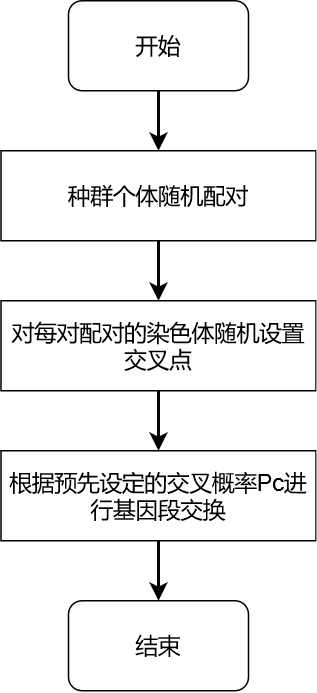
\includegraphics[width = 0.2\textwidth]{onepoint_cross.drawio.png}
  \caption{单点交叉流程图}
  \label{fig:onepoint_corss}
\end{figure}

其他类型的交叉操作还有双点和均匀交叉技术。双点交叉在匹配的染色体上随机确定两个位置,并将这两个位置之间的染色体段进行交换,以此来调整基因序列。
均匀交叉则对配对染色体上的每一个基因位都以相同的概率进行交叉,生成新的基因组合。
算术交叉通过对配对染色体执行线性组合的交叉,以产生变化的基因序列。
\begin{figure}[h]
  \centering
  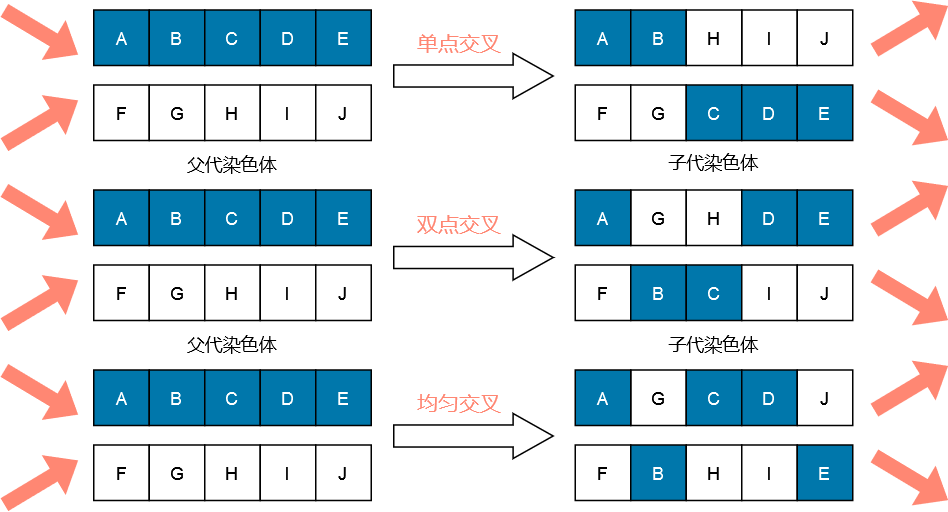
\includegraphics[width = 0.8\textwidth]{crossshow.drawio.png}
  \caption{交叉操作示意图}
  \label{fig:cross_show}
\end{figure}

变异:
为避免遗传算法过早收敛至局部最优,变异操作被引入以增强搜索的多样性。在应用中,常用的是单点变异,亦称位变异。
单点变异随机选取染色体上的一个基因位,并反转其值:若为二进制编码,则将0改为1,1改为0。
\begin{figure}[h]
  \centering
  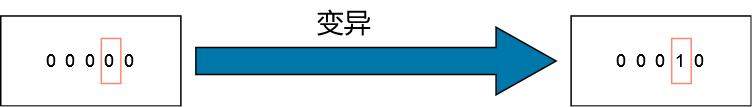
\includegraphics[width = 0.8\textwidth]{mutate.drawio.png}
  \caption{变异操作示意图}
  \label{fig:mutate}
\end{figure}

群体$P(t)$经过选择、交叉、变异运算后得到下一代群体$P(t+1)$。
若$t\leq T$,则 $t \leftarrow t + 1$,重新计算适应值;否则以进化过程中所得到的具有最大适应度的个体作为最好的解输出,终止运算。
图~\ref{fig:ga_procedure}~是整个遗传算法的流程图。
\begin{figure}[h]
  \centering
  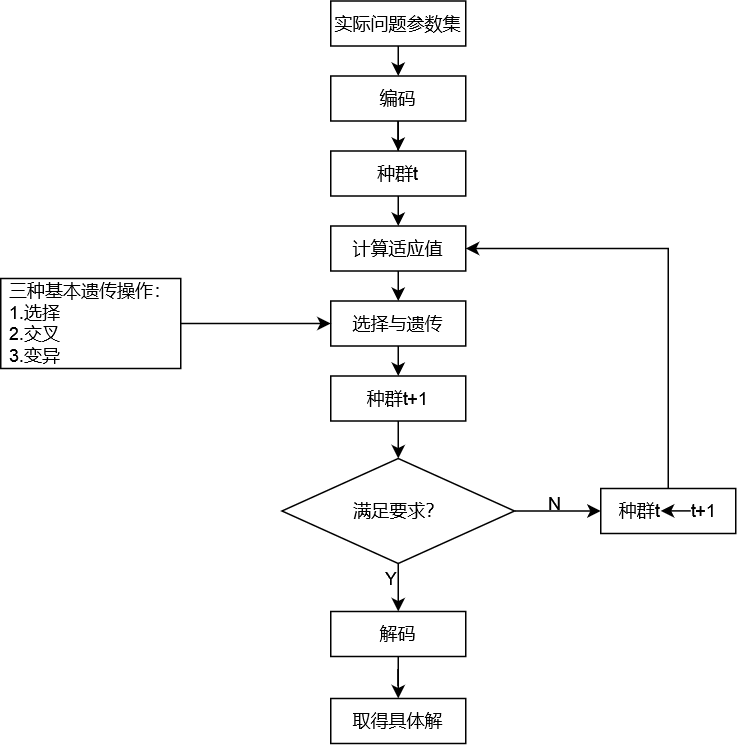
\includegraphics[width = 0.8\textwidth]{ga_procedure.drawio.png}
  \caption{遗传算法流程图}
  \label{fig:ga_procedure}
\end{figure}




%%================================================
%% Filename: chap04.tex
%% Encoding: UTF-8
%% Author: Yuan Xiaoshuai - yxshuai@gmail.com
%% Created: 2012-04-28 00:15
%% Last modified: 2019-11-06 17:39
%%================================================
\chapter{基于特征融合的增量学习异常流量检测模型}
% \chapter{基于多模态特征融合的增量学习方案}
\label{cha:ResNet-BiGRU}

由于传统的网络攻击检测方法不能综合分析网络流量数据中的空间特征与时序特征,网络攻击检测的准确性仍有很大的提升空间。
因此,本文设计并提出了一个基于残差网络与双向门控循环单元的多模态特征融合模型(ResNet-BiGRU based Multimodal Fusio,RB-MF),旨在充分挖掘流量数据时空特征的同时,对其综合分析,进一步提高模型准确率。
此外,针对传统攻击检测技术在应对新型攻击时表现出的检测能力不足、难以适应攻击模式不断变化的问题,本文进一步提出了一个基于多模态特征融合的增量学习方案。
本方案在保留模型原有知识的基础上,使其具备持续适应和学习新攻击模式的能力,进而逐步适应日新月异的攻击环境,确保安全防护的时效性和准确性。

% \section{方案概述}
图~\ref{fig:attack_detecion_model}~描述了本文方案的工作原理和流程。
\begin{figure}[h]
	\centering
	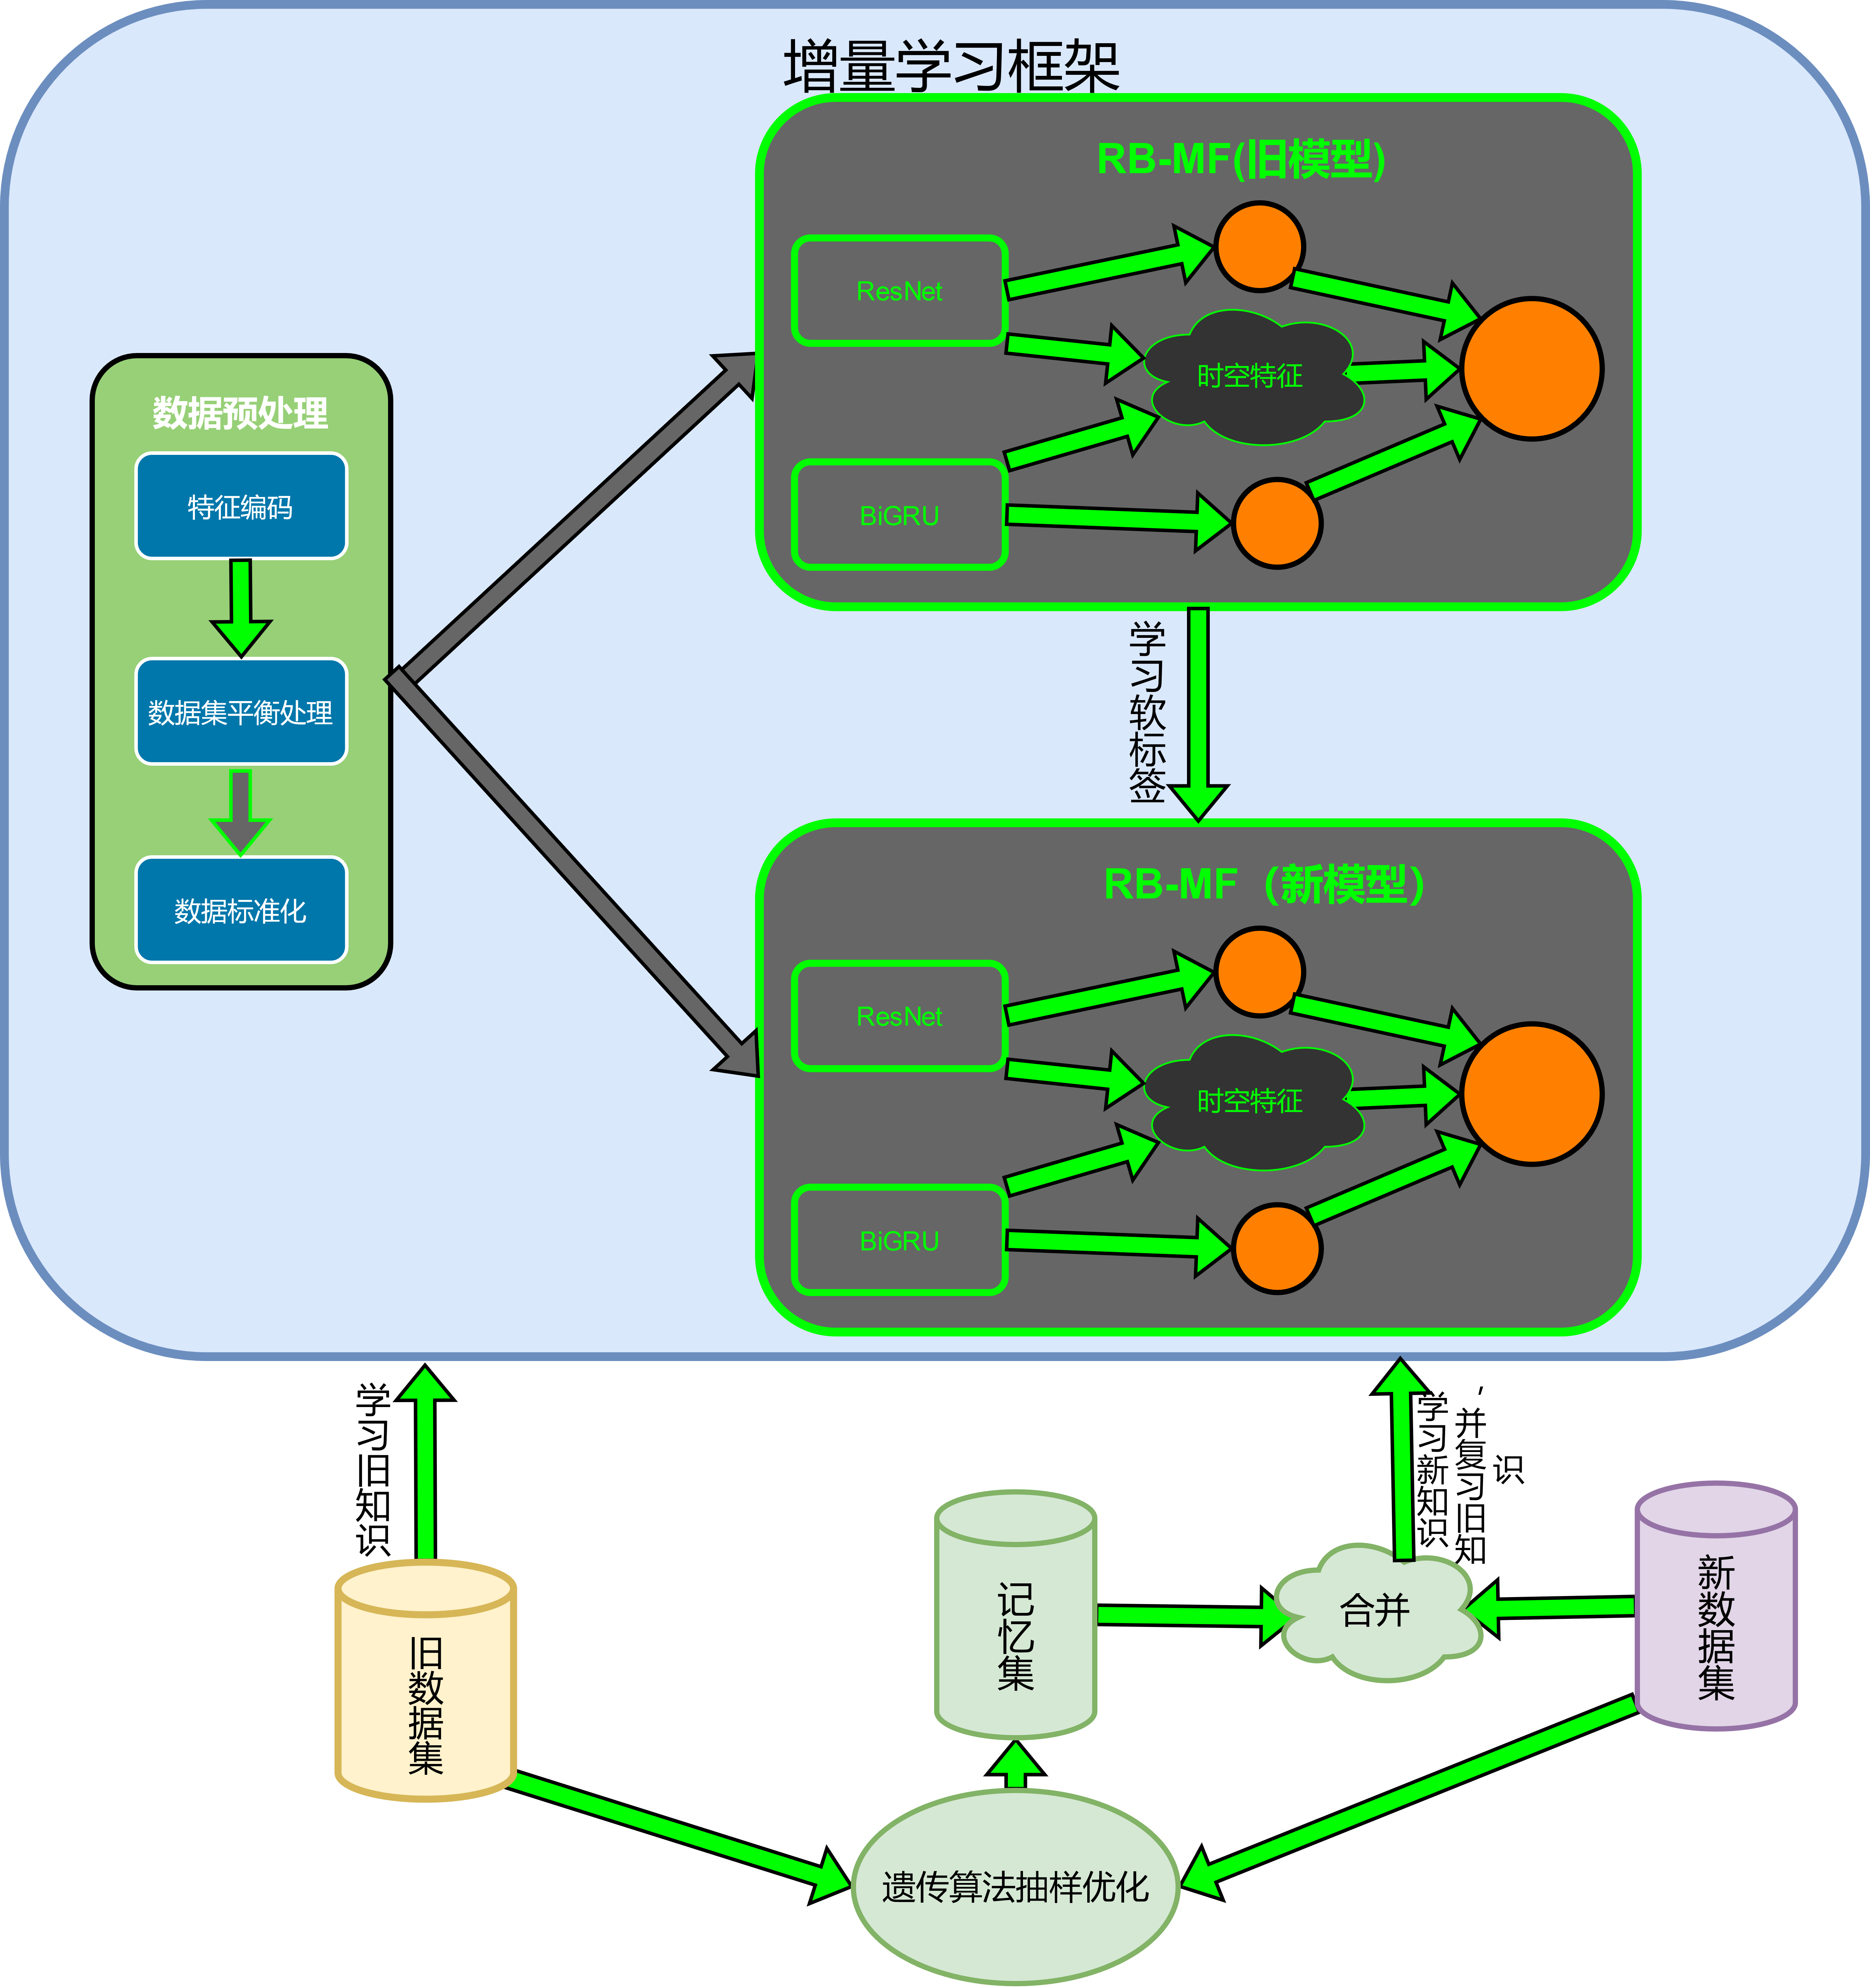
\includegraphics[width = 0.74\textwidth]{chapter_4.drawio.png}
	\caption{基于多模态特征融合的增量学习方案原理及流程}
	\label{fig:attack_detecion_model}
\end{figure}
基于多模态特征融合的增量学习方案由以下四个关键部分构成:首先是RB-MF模型的结构设计,其次是数据集的预处理流程,再次是RB-MF模型的增量学习策略,最后是记忆集的抽样优化方法。
首先,第一部分是本文接下来将要提出的RB-MF模型的设计与实现,该模型能够综合分析流量数据集的时空特征,在攻击检测准确率方面具有很好的表现。
第二部分对数据集进行预处理,确保RB-MF模型能够顺利地进行训练和测试。
第三部分在RB-MF模型完成旧任务数据的训练后,结合iCaRL\cite{rebuffi2017icarl}策略使RB-MF模型具备持续学习和适应新环境的能力。
最后一部分则利用遗传算法实现iCaRL策略中记忆集的分层抽样优化,使得RB-MF模型在固定大小的记忆集上最大化记忆能力。

\section{基于特征融合的异常流量检测模型}
% 网络通信涉及复杂的交互模式,包括客户端与服务器之间的请求响应、数据传输过程中的拥塞控制等。
% 这些交互在空间上体现为数据包的具体内容,如源IP地址、目标IP地址、端口号、协议类型等,这些信息在数据包的特定位置以特定格式存在,形成了数据的“空间”结构。
% 在时间上则表现为交互的顺序和持续时间。\par
该模型的原理是通过多模态特征融合技术将ResNet以及BiGRU进行融合,从而综合分析网络流量数据中的时空特性,提升决策性能。
其具体流程为,首先,ResNet提取网络流量数据中的深层次空间特征,BiGRU则捕捉流量数据时序特征的前后依赖关系。
接着,结合这两个特征形成混合的“时空特征”。
最后,综合ResNet和BiGRU的决策输出以及“时空特征”,结合三者,产生最终的决策输出。
\subsection{多模态特征融合设计}
多模态特征融合是一种将来自不同来源或类型(模态)的数据集成在一起的过程,目的是改善决策过程提高预测准确性。
这些不同模态的数据可能包括文本、图像、视频、音频和传感器数据等。
在机器学习和深度学习领域,多模态特征融合已成为一个重要的研究领域,尤其是在那些需要综合处理不同类型数据的应用中,如自然语言处理、计算机视觉、语音识别和人机交互等。
融合策略通常可以分为早期融合、晚期融合、混合融合三种类型\cite{hejunandzhangcaiqing}。\par

早期融合(如图~\ref{fig:MultimodalFusio} (a)~所示),也被称为特征级融合,其核心思想是在模型的某个中间层将不同模态的特征进行集成。
这种策略充分利用了深度学习模型在捕捉和利用模态间交互作用方面的能力。\par

晚期融合(如图~\ref{fig:MultimodalFusio} (b)~所示)则采取了另一种思路。
在这种策略中,每个模态都单独处理并产生决策,而最终的融合则发生在决策层面,通常通过投票机制、平均值计算或是基于学习的加权组合等方式来实现。
晚期融合的优点在于能够保持模态间的独立性,适用于模态间关联较弱的情况。\par

混合融合(如图~\ref{fig:MultimodalFusio} (c)~所示)策略则更为灵活,它结合了早期融合和晚期融合的优点,旨在在特征提取和决策过程中充分利用各种融合方法的优势。
例如,一个混合融合框架可能同时利用早期融合来捕捉模态间的直接联系,同时借助晚期融合来维持某些模态的独立性,从而确保信息处理的全面性和准确性。
这种策略不仅提升了融合效果,也增强了模型的鲁棒性和泛化能力。\par

\begin{figure}[h]
	\centering
	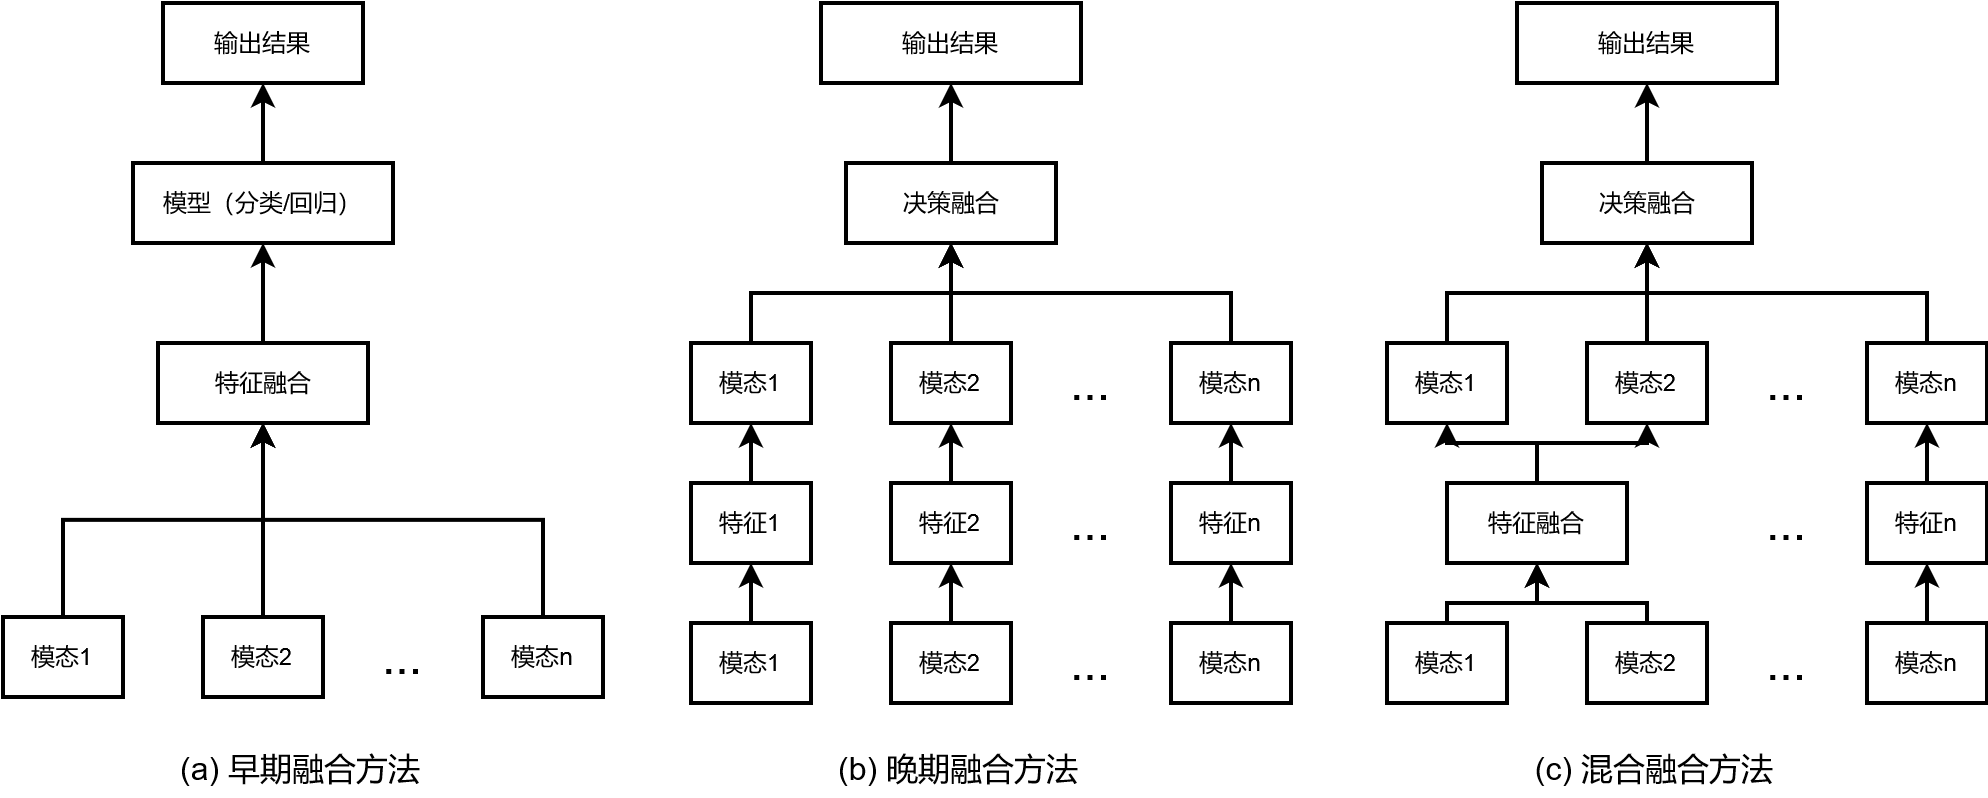
\includegraphics[width = \textwidth]{MultimodalFusion.drawio.png}
	\caption{3种多模态特征融合方法}
	\label{fig:MultimodalFusio}
\end{figure}


早期融合的效果在很大程度上取决于对模态特性的理解和模型结构设计。
然而,由于不同模态数据的多样性和复杂性,早期融合可能并不总是适用于所有类型的多模态数据。
在某些情况下,不恰当的融合方式可能会导致信息丢失或模型性能下降。
晚期融合虽然能够保持模态之间的独立性,但由于每个模态是独立处理的,它可能无法充分捕获模态之间的深层次相互作用。
此外,晚期融合通常在决策层面进行,这在一定程度上限制了对不同模态特征之间更细粒度关系的探索和利用。
相比之下,混合融合策略通过结合早期融合和晚期融合的优点,为模型设计提供了更大的灵活性和适应性。
它能够在不同的层级和阶段整合不同模态的信息,从而最大化地利用不同模态之间的互补性和关联性。这种策略不仅能够捕获模态之间的直接特征信息,还能够挖掘深层次的相互作用信息,进一步提升模型的性能。\par



因此,本文将会利用混合融合策略来整合ResNet和BiGRU模型的优势。
首先,我们将分别利用ResNet和BiGRU来从网络流量数据集中提取空间特征和时序特征。
ResNet的强大之处在于其深度结构和残差连接,使其能够捕捉到网络流量数据中的复杂空间模式;而BiGRU则通过其双向结构,有效地捕获了时序数据中的长期依赖关系。
接着,为了高效且有效地融合这两种特征,我们采用联合架构。
联合架构有两种融合方法,即“加”联合方法和“乘”联合方法。
“加”联合方法,也称为加法融合,是一种直观且计算效率高的方式。它通过对不同模态的特征向量进行加权和或简单的相加操作来融合特征。
这种方法基于一个假设,即不同模态的特征贡献可以直接相加,从而形成一个综合的特征表示。
加法融合不仅易于实现,而且能够保留原始特征中的大部分信息,同时减少了计算复杂度。
加法融合可以表示为:
\begin{equation}
	z = f(w_1^Tv_1 + w_2^Tv_2+ \dots + w_n^Tv_n)
\end{equation}
\begin{flushleft}
	\renewcommand\arraystretch{1.25}
	\begin{tabularx}{\textwidth}{@{}>{\normalsize\rm}l@{\quad}>{\normalsize\rm}l@{——}>{\normalsize\rm}X@{}}
		式中 & $z$ & 共享语义子空间的输出结果;                                              \\
		     & $N$ & 类别总数;                                                              \\
		     & $v$ & 各模态的输入;                                                          \\
		     & $w$ & 权重,下标表示不同的模态,通过映射$f$将所有子模态语义转换到共享子空间。 \\
	\end{tabularx}\vspace{.5ex}
		式中 & $z$ & 共享语义子空间的输出结果;                                              \\
		     & $N$ & 类别总数;                                                              \\
		     & $v$ & 各模态的输入;                                                          \\
		     & $w$ & 权重,下标表示不同的模态,通过映射$f$将所有子模态语义转换到共享子空间。 \\
	\end{tabularx}\vspace{.5ex}
\end{flushleft}


"乘"联合方法,或乘法融合,涉及到对不同模态的特征进行乘积操作。
这种方法基于这样的假设:一个模态的特征可以通过与另一模态的特征进行乘积来增强或抑制重要的信号。
乘法联合可以用以下公式表示:
\begin{equation}
	z = \begin{bmatrix}v^1 \\1\\\end{bmatrix} \otimes \begin{bmatrix}v^2 \\1\\\end{bmatrix} \otimes \dots \otimes \begin{bmatrix}v^n \\1\\\end{bmatrix}
\end{equation}
\begin{flushleft}
	\renewcommand\arraystretch{1.25}
	\begin{tabularx}{\textwidth}{@{}>{\normalsize\rm}l@{\quad}>{\normalsize\rm}l@{——}>{\normalsize\rm}X@{}}
		式中 & $z$       & 融合张量后的结果输出; \\
		     & $v$       & 不同的模态;           \\
		     & $\otimes$ & 外积算子。             \\
	\end{tabularx}\vspace{.5ex}
		     & $v$       & 不同的模态;           \\
		     & $\otimes$ & 外积算子。             \\
	\end{tabularx}\vspace{.5ex}
\end{flushleft}



尽管“加”联合方法具有简单性和易实现性的优势,但它可能因特征向量语义组合的局限性而导致后期语义信息的丢失,进而影响模型性能。
相对而言,“乘”联合方法通过张量计算的方式,能够更加深入地融合特征语义,弥补“加”联合方法的不足\cite{hejunandzhangcaiqing}。
因此,为了更全面地融合ResNet和BiGRU提取的空间与时序特征,本文将采用“乘”联合方法来进行特征融合。
这种方法能够确保特征语义在融合过程中得到充分保留和增强,从而有望提高模型的准确性和鲁棒性。\par

最终,本文所构建的融合架构如图~\ref{fig:ResNet-BiGRU-Fusion}~所示。
\begin{figure}[htbp]
	\centering
	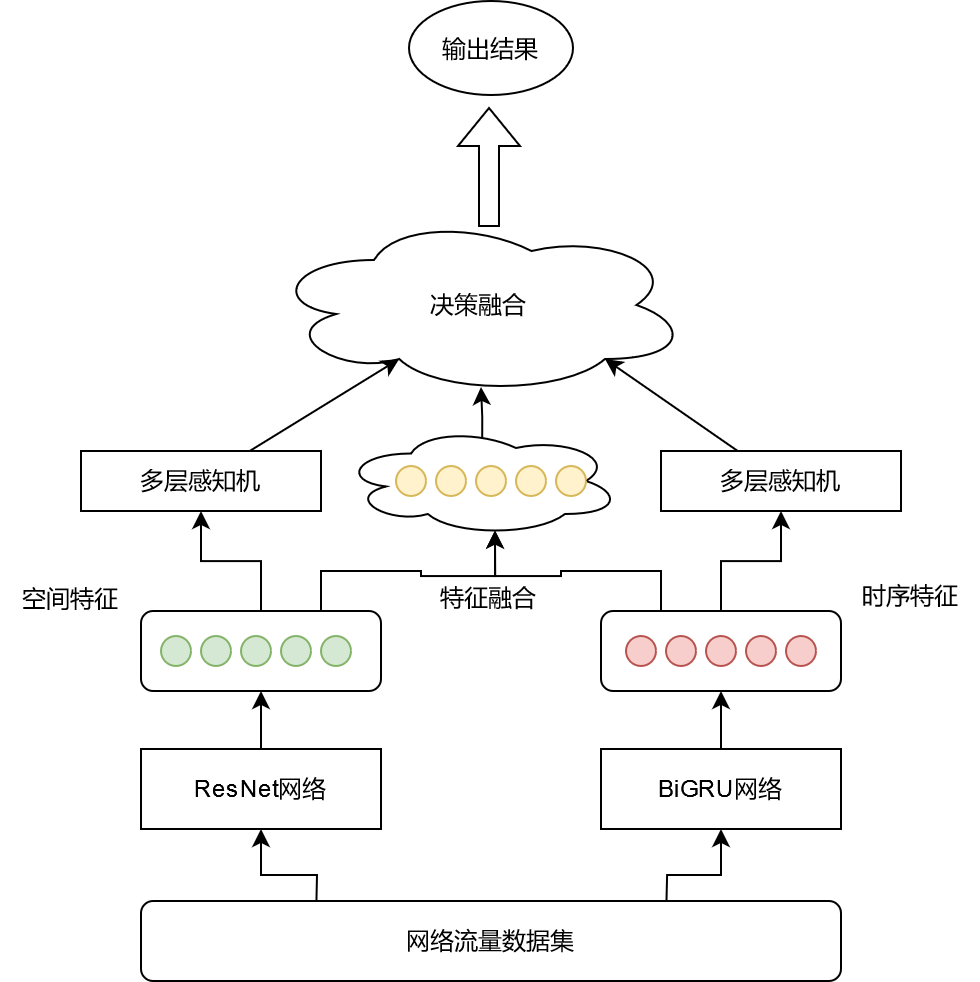
\includegraphics[width = 0.7\textwidth]{ResNet-BiGRU-Fusion.drawio.png}
	\caption{ResNet-BiGRU特征融合设计}
	\label{fig:ResNet-BiGRU-Fusion}
\end{figure}
该架构充分利用了混合融合策略的优势,通过结合ResNet和BiGRU的特征提取能力,并采用“乘”联合方法进行特征融合,为网络流量分析等相关任务提供了强大的支持。

\subsection{模型网络结构设计}
本文的融合模型核心在于残差网络与双向门控循环单元网络的结合,并通过独特的多模态特征融合策略实现两者间的有效协同。
% 本文的融合模型主要由一个残差网络以及一个双向门控循环单元网络以及它们之间的多模态特征融合方式构成。
其中,残差模型主要包括两种类型的残差块:conv\_block(卷积残差块)和identity\_block(恒等残差块)。
这两种块的设计旨在解决深度神经网络训练中常见的梯度消失问题,从而使网络能够在增加深度的同时保持训练的有效性和稳定性。
conv\_block负责调整输入特征图的维度,以匹配块输出时的维度变化。
它通过在残差路径中引入具有步长的卷积操作来实现降维,并通过额外的卷积层来调整通道数,从而使得主路径上的特征图尺寸与残差路径上的输出能够相匹配。
这种设计使得网络能够在增加深度的同时,适应更高层的特征表示。
identity\_block则在不需要改变输入特征图维度时使用,主要用于网络的深层部分,用以加深网络深度提高模型的性能。\par

残差模型以15x15\footnote{特征编码后,数据维度变为(214,1)。为进行2D卷积,本文将其调整为(15,15,1)并进行了零填充。}的二维输入数据开始,紧接着是一个初始卷积层,该层使用64个3x3大小的滤波器,并应用’same’填充,以保持输出特征图的尺寸。
此外,这一层使用L2正则化以防止过拟合,并通过批归一化(BatchNormalization)和ReLU激活函数对特征进行标准化和非线性化处理。

接下来,模型通过两个阶段的残差块处理特征:

\begin{enumerate}[label=\arabic*)]
	\item 第一阶段包含一个conv\_block和一个identity\_block,分别用于特征图的尺寸和深度调整以及模型深度的增加。
	\item 第二阶段则起始于另一个conv\_block,随后是两个identity\_block,以进一步增强模型的特征提取能力。
\end{enumerate}
每个卷积层都配备了L2正则化,且所有残差块后都跟随批归一化和ReLU激活函数,以促进有效训练并避免梯度问题。

在经过残差块序列处理后,模型使用平均池化层(AveragePooling2D)来减小特征图的尺寸,随后是一个Dropout层,以0.5的比率随机断开输入单元,降低过拟合的风险。
最后,模型将处理后的特征展平,为与BiGRU的时序特征融合做准备。表~\ref{tab:resnet_description}~是该残差网络的具体结构。


\begin{table}[h]
	\caption{残差网络模型结构}
	\label{tab:resnet_description}
	\centering
	\begin{tabular}{c|c|c}
		\hline
		Layer name                & Output size                              & ResNetPart             \\
		\hline
		conv1                     & $15 \times 15$                           & $3\times3$, 64, stride 1 \\
		\hline
		% 使用multirow和mbox命令来确保矩阵居中
		\multirow{4}{*}{conv2\_x} & \multirow{4}{*}{\centering $8 \times 8$} &
		\multirow{4}{*}{$\left[\begin{array}{c}
						1 \times 1, 64 \\
						3 \times 3, 64 \\
						1 \times 1, 256
					\end{array}\right] \times 2$ , stride 2}                  \\
						1 \times 1, 64 \\
						3 \times 3, 64 \\
						1 \times 1, 256
					\end{array}\right] \times 2$ , stride 2}                  \\
		                          &                                          &                          \\
		                          &                                          &                          \\
		                          &                                          &                          \\
		\hline
		\multirow{4}{*}{conv3\_x} & \multirow{4}{*}{\centering $8 \times 8$} &
		\multirow{4}{*}{$\left[\begin{array}{c}
						1 \times 1, 64 \\
						3 \times 3, 64 \\
						1 \times 1, 256
					\end{array}\right] \times 2$, stride 1}                   \\
						1 \times 1, 64 \\
						3 \times 3, 64 \\
						1 \times 1, 256
					\end{array}\right] \times 2$, stride 1}                   \\
		                          &                                          &                          \\
		                          &                                          &                          \\
		                          &                                          &                          \\
		\hline
		avg\_pool                 & $1 \times 1$                             & AvgPool $2 \times 2$     \\
		\hline
		flatten                   & 1,1264                                   &                          \\
		\hline
		dropout                   &                                          & Dropout(0.5)             \\
		\hline
	\end{tabular}
\end{table}


对于BiGRU模型,第一层包含64个单元,用于捕捉序列数据的时序依赖关系,并保留每个时间步的输出。这一设计旨在充分提取序列中的动态特征。
为了降低模型过拟合的风险,我们在第一层BiGRU后引入了一个10\%的dropout层,通过随机丢弃部分特征连接来增强模型的泛化能力。
随后,数据进入第二个BiGRU层,该层拥有32个单元,专注于捕捉更深层次的时序信息。与第一层不同,这一层仅输出最后一个时间步的结果,以捕捉序列的整体趋势。
随后是另一个10\%的dropout层,以进一步减少过拟合。
值得注意的是,为了将BiGRU层的特征输出与ResNet模型的特征进行合并,在这个结构中也同样并没有加入全连接层(Dense layer)作为输出。\par


最终,我们从ResNet模型和BiGRU模型中分别提取特征,并通过特定的融合策略进行合并。
此外,为了与BiGRU的输出维度相匹配,我们将ResNet的输出从11264维通过适当的映射降维至64维。
随后,采用元素乘法操作将两种模型的特征进行融合,确保不同模态的信息能够相互补充。
在特征融合后,我们将ResNet和BiGRU的决策输出与融合特征合并成一个统一的张量。这一张量随后通过一个额外的Dense层进行进一步处理,最终输出分类决策。
通过这一设计,我们能够充分利用ResNet和BiGRU各自的优势,并通过混合融合策略实现多模态特征的有效整合。

图~\ref{fig:hyber_model_struct}~是这个混合模型的整体架构,表~\ref{tab:model_params}~是混合模型的参数数量。
\begin{figure}[h]
	\centering
	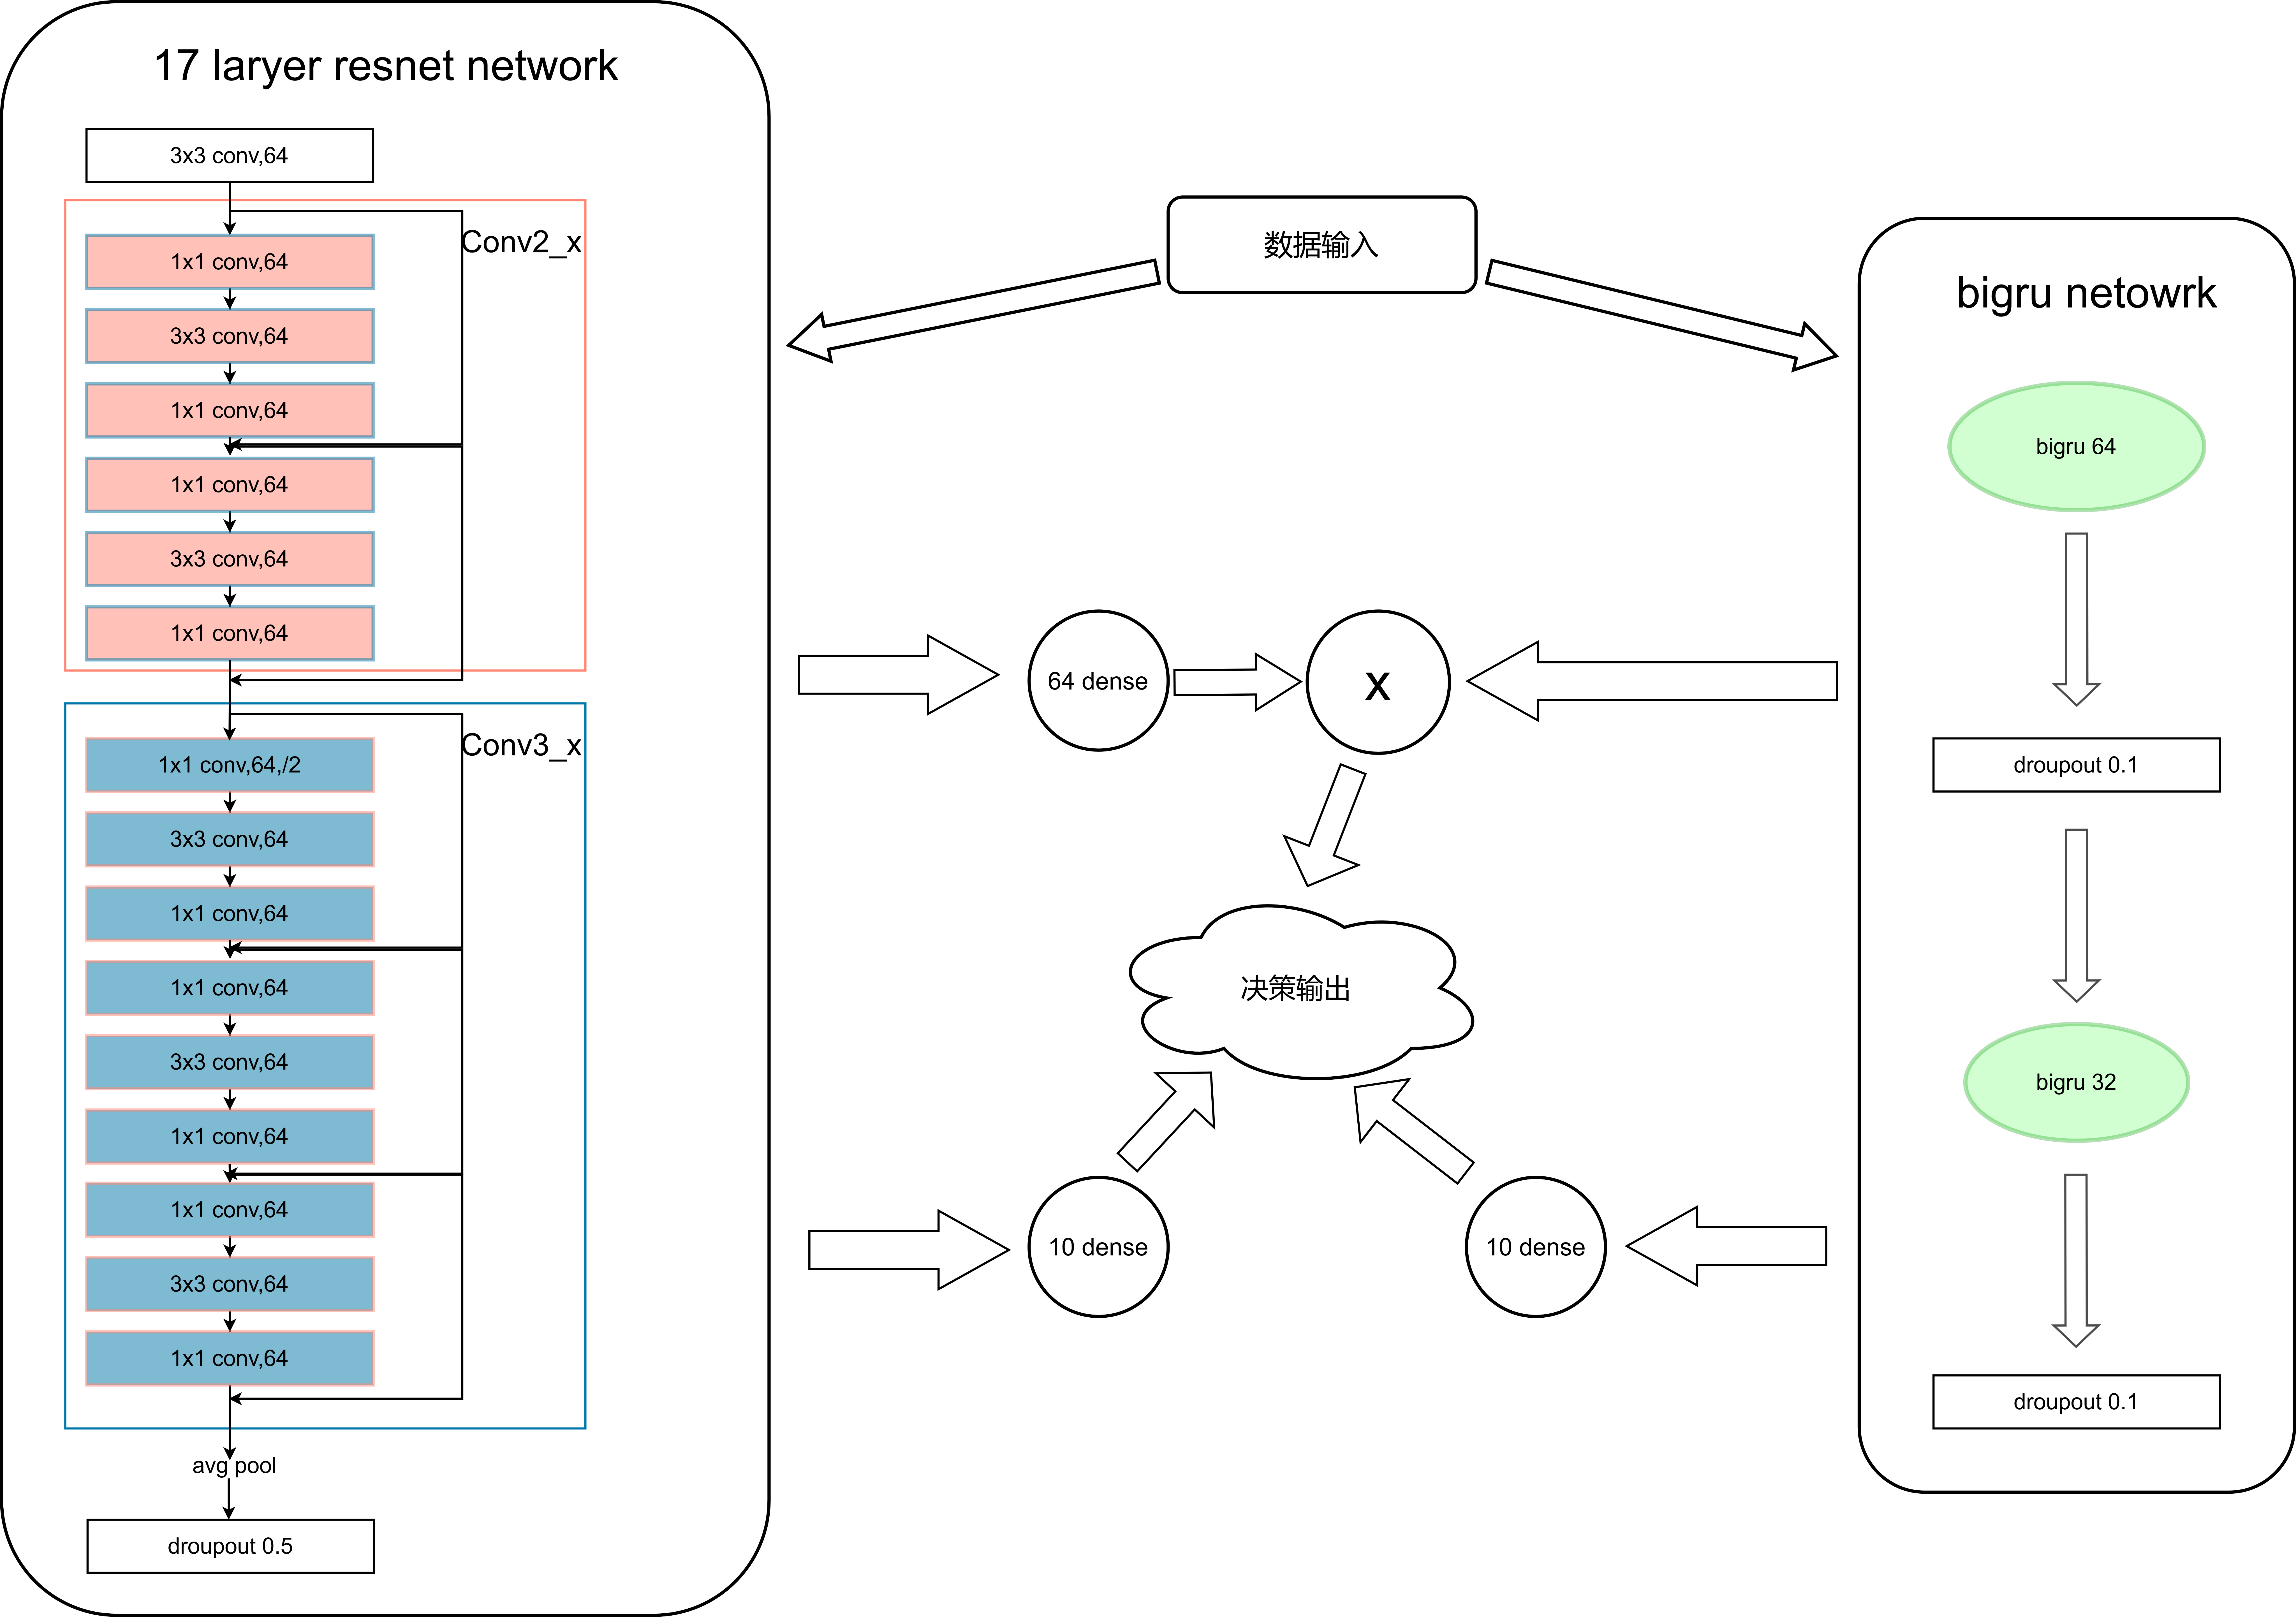
\includegraphics[width = \textwidth]{hyber_model_struction.drawio.png}
	\caption{混合模型整体结构}
	\label{fig:hyber_model_struct}
\end{figure}



\begin{table}[h]
	\caption{混合模型参数数量}
	\label{tab:model_params}
	\centering
	\begin{tabular}{ccc}
		\toprule
		\textbf{总参数} & \textbf{可训练参数数量} & \textbf{非可训练参数数量} \\
		\midrule
		1,417,510       & 1,412,518               & 4,992                     \\
		1,417,510       & 1,412,518               & 4,992                     \\
		\bottomrule
	\end{tabular}
\end{table}
\subsection{数据预处理}
数据预处理是深度学习及机器学习中的关键环节,它对于构建一个干净、标准化且均衡的数据集至关重要。
预处理的主要目标是为后续的特征学习和模型训练奠定坚实的基础。
通过实施恰当的数据预处理策略,我们能够显著提升模型的性能、加速训练过程,并增强模型对未见数据的泛化能力。\par

以下是本文的数据预处理步骤:首先,我们对训练集和测试集进行特征编码,以确保分类数据能够被模型有效处理;
随后,我们针对原始数据集及编码过程中可能出现的缺失值进行了详尽的处理,以确保数据的完整性和准确性;
鉴于本文所使用的数据集存在显著的类别不平衡问题,我们还将对少数类样本进行过采样处理。
这一策略旨在平衡训练过程中的类别表示,从而提升模型对少数类的识别能力。
通过这一系列预处理步骤,我们有望构建一个更加优质的数据集,为后续的模型训练提供有力支持。\par

图~\ref{fig:dataprocess}~概括性地展示了整个数据预处理流程。
本节接下来的部分将对这一流程中的关键步骤进行详细阐述,以便于读者深入理解本文采取的方法及其背后的逻辑。
\begin{figure}[htbp]
	\centering
	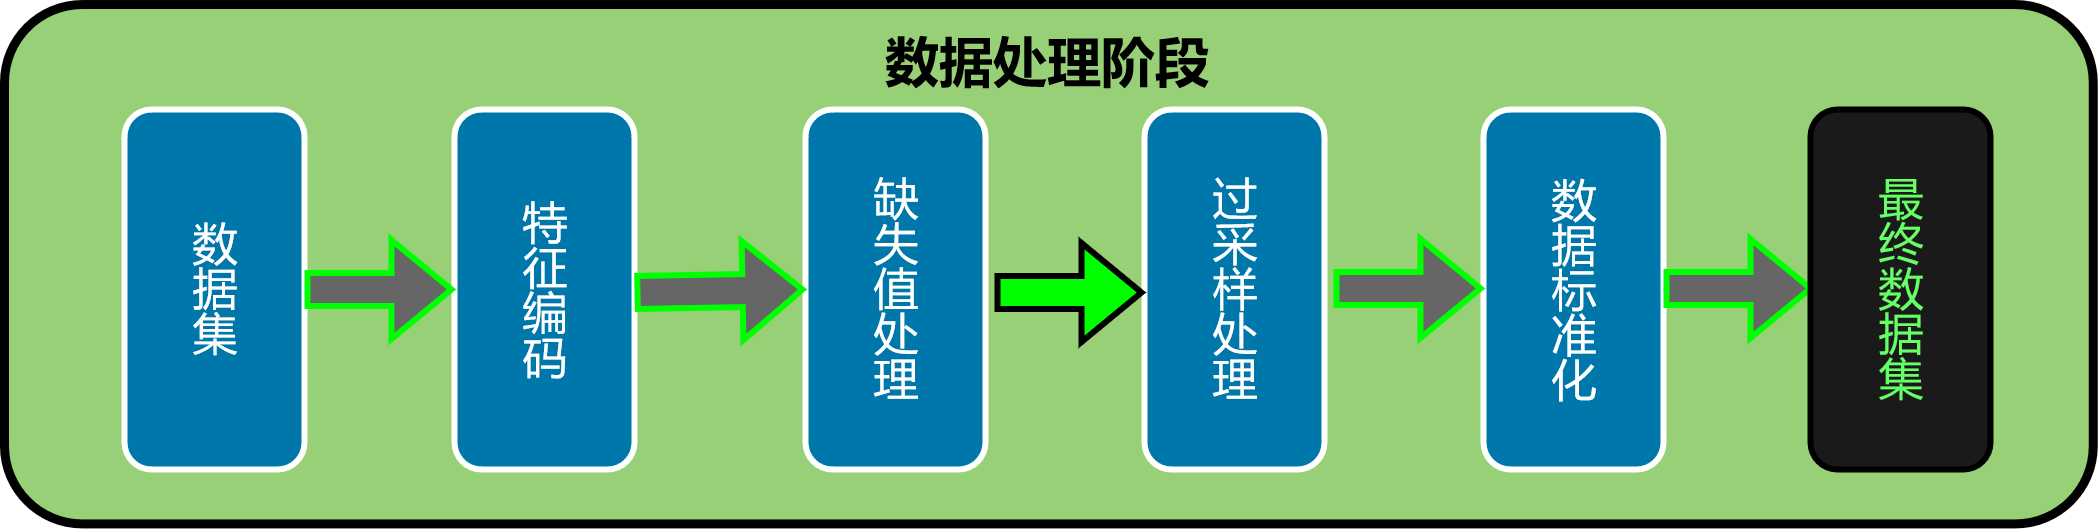
\includegraphics[width = 0.8\textwidth]{dataprocess.drawio.png}
	\caption{数据集预处理流程图}
	\label{fig:dataprocess}
\end{figure}

1)~特征编码\par

特征编码是数据预处理中不可或缺的一环,旨在将原始数据转化为模型能够识别和处理的数值格式。
这个过程对于提高模型的性能和准确性至关重要,因为大多数模型的预期输入数据为数值型,而原始数据往往包括各种类型,如文本、日期或分类数据。
特征编码目的便是将非数值特征转换为数值形式,使模型能够对这些数据进行计算。
在我们的流量数据集中,同样存在大量非数值类型的特征,如IP地址、协议类型等。
为了充分利用这些数据并构建有效的模型,我们需要对这些非数值特征进行特征编码,将其转换为数值类型。\par

One-Hot 编码是一种特殊且广泛使用的特征编码方法,它易于理解和实现,非常适用于处理具有有限类别的分类数据。
鉴于其实施简便性,本文决定采用One-Hot 编码方式,针对数据集中的非数值类型特征进行转换。
该方法的工作原理是为每个类别创建一个独立的二进制列,这样每个数据点在其所属类别的对应列上被标记为1,而在其他所有列上则被标记为0。
通过这种方式,我们能够有效地将非数值类型特征转换为机器学习算法易于处理的数值形式,从而提升模型的性能。
表~\ref{tab:onehot}~是这一方法的具体算法。\par
\begin{table}[htbp]
	\caption{One-hot编码算法实现}
	\label{tab:onehot}
	\centering
	\begin{tabularx}{1.0\textwidth}{cl}
		\toprule
		\multicolumn{2}{l}{\textbf{one-hot编码算法}}                              \\
		\midrule
		\multicolumn{2}{l}{\textbf{输入}: 数据集 $D$,其中包含数值型和分类型列}   \\
		\multicolumn{2}{l}{\textbf{输出}: 经过One-hot编码的数据集 $D'$}           \\
		1  & 初始化一个空的数据集 $D'$                                            \\
		2  & \textbf{for} 每一列 $col$ \textbf{in} $D$:                           \\
		\multicolumn{2}{l}{\textbf{输入}: 数据集 $D$,其中包含数值型和分类型列}   \\
		\multicolumn{2}{l}{\textbf{输出}: 经过One-hot编码的数据集 $D'$}           \\
		1  & 初始化一个空的数据集 $D'$                                            \\
		2  & \textbf{for} 每一列 $col$ \textbf{in} $D$:                           \\
		3  & \quad \textbf{if} $col$ 是分类型:                                    \\
		4  & \quad\quad $unique\_values$ = 获取 $col$ 的所有唯一值                \\
		4  & \quad\quad $unique\_values$ = 获取 $col$ 的所有唯一值                \\
		5  & \quad\quad \textbf{for} 每一个值 $val$ \textbf{in} $unique\_values$: \\
		6  & \quad\quad\quad 创建一个新列 $new\_col$,名称为 ``$col\_val$''       \\
		7  & \quad\quad\quad \textbf{for} 每一行 $row$ \textbf{in} $D$:           \\
		8  & \quad\quad\quad\quad \textbf{if} $row[col] == val$:                  \\
		6  & \quad\quad\quad 创建一个新列 $new\_col$,名称为 ``$col\_val$''       \\
		7  & \quad\quad\quad \textbf{for} 每一行 $row$ \textbf{in} $D$:           \\
		8  & \quad\quad\quad\quad \textbf{if} $row[col] == val$:                  \\
		9  & \quad\quad\quad\quad\quad 在 $D'[new\_col]$ 中填充 1                 \\
		10 & \quad\quad\quad\quad \textbf{else}:                                  \\
		10 & \quad\quad\quad\quad \textbf{else}:                                  \\
		11 & \quad\quad\quad\quad\quad 在 $D'[new\_col]$ 中填充 0                 \\
		12 & \quad \textbf{else}:                                                 \\
		13 & \quad\quad 将 $col$ 直接复制到 $D'$ 中                               \\
		14 & \textbf{return} $D'$                                                 \\
		12 & \quad \textbf{else}:                                                 \\
		13 & \quad\quad 将 $col$ 直接复制到 $D'$ 中                               \\
		14 & \textbf{return} $D'$                                                 \\
		\bottomrule
	\end{tabularx}
\end{table}

在处理IP地址时,直接进行One-Hot编码会破坏其内在特征并导致维度爆炸,影响模型性能。
常见的处理方法包括字段分割、整数转换、地理定位和嵌入法。字段分割法将IPv4地址拆分为四个数值特征,保留模式识别能力。
整数转换法将IP转为32位整数(IPv6为更大整数),保持层次结构,适合数值特征处理。
地理定位将IP映射到地理特征,如国家、城市,利用外部服务获取,适用于地域分析。
嵌入法通过深度学习将IP转换为向量,捕获地址间相似性,但计算成本高。
考虑到整数法可能引起特征不平衡,地理定位操作复杂,嵌入法计算代价大,本文采用字段分割法简化处理流程。\par

2)~数据集平衡处理\par
在大规模数据集预处理中,解决数据不平衡问题是提高模型性能和泛化能力的关键步骤。
由于本文采用的数据集是非常不均衡的,本文将会对数据集进行平衡处理。
数据不平衡通常通过欠采样和过采样两种重采样策略来处理。
欠采样通过减少多数类样本来达到平衡,虽然助于增强模型对少数类的关注,但会造成信息丢失。
相反,过采样则通过增加少数类样本数量来平衡数据,例如可以采用复制样本或利用SMOTE等高级技术生成新样本,提高少数类的代表性。\par

SMOTE(Synthetic Minority Over-sampling Technique)是一种过采样策略,通过合成新的少数类样本而非简单重复现有样本来平衡数据集。
其核心优势在于增加数据多样性,促进模型学习复杂决策边界,显著提升分类器对少数类的识别能力,改善模型性能和泛化能力。
在样本量不足时,过采样尤为适用,鉴于此,本文将会利用SMOTE算法对数据集进行平衡处理,以期提升模型的分类效果。
表~\ref{tab:smote}~是该技术的算法实现。
\begin{table}[htbp]
	\caption{SMOTE算法实现}
	\label{tab:smote}
	\centering
	\begin{tabularx}{1.0\textwidth}{cl}
		\toprule
		\multicolumn{2}{l}{\textbf{SMOTE算法}}                                              \\
		\multicolumn{2}{l}{\textbf{SMOTE算法}}                                              \\
		\midrule
		\multicolumn{2}{l}{\textbf{输入}: 少数类样本集 $S$,采样倍率 $N$,最近邻数 $k$}     \\
		\multicolumn{2}{l}{\textbf{输入}: 少数类样本集 $S$,采样倍率 $N$,最近邻数 $k$}     \\
		\multicolumn{2}{l}{\textbf{输出}: 合成样本集 $S'$}                                  \\
		1  & 如果 $N$ 不是整数,则将 $N$ 向下取整,同时调整最终的样本数量                   \\
		2  & 初始化空的合成样本集 $S'$                                                      \\
		3  & \textbf{for} 每一个样本 $s$ \textbf{in} $S$:                                   \\
		1  & 如果 $N$ 不是整数,则将 $N$ 向下取整,同时调整最终的样本数量                   \\
		2  & 初始化空的合成样本集 $S'$                                                      \\
		3  & \textbf{for} 每一个样本 $s$ \textbf{in} $S$:                                   \\
		4  & \quad 找到 $s$ 的 $k$ 个最近邻                                                 \\
		5  & \quad \textbf{for} $i$ \textbf{from} 1 \textbf{to} $N$:                        \\
		6  & \quad\quad 随机选择一个最近邻 $nn$                                             \\
		7  & \quad\quad \textbf{for} 每个特征 $f$:                                          \\
		8  & \quad\quad\quad 计算 $s$ 和 $nn$ 在特征 $f$ 上的差值 $\Delta f$                \\
		5  & \quad \textbf{for} $i$ \textbf{from} 1 \textbf{to} $N$:                        \\
		6  & \quad\quad 随机选择一个最近邻 $nn$                                             \\
		7  & \quad\quad \textbf{for} 每个特征 $f$:                                          \\
		8  & \quad\quad\quad 计算 $s$ 和 $nn$ 在特征 $f$ 上的差值 $\Delta f$                \\
		9  & \quad\quad\quad 生成新值 $new\_f = s[f] + \Delta f \times \text{随机数}(0, 1)$ \\
		10 & \quad\quad 创建新样本 $new\_s[i]$,其特征值为所有生成的 $new\_f$               \\
		11 & \quad\quad 将 $new\_s[i]$ 添加到合成样本集 $S'$                                \\
		12 & \textbf{return} $S'$                                                           \\
		10 & \quad\quad 创建新样本 $new\_s[i]$,其特征值为所有生成的 $new\_f$               \\
		11 & \quad\quad 将 $new\_s[i]$ 添加到合成样本集 $S'$                                \\
		12 & \textbf{return} $S'$                                                           \\
		\bottomrule
	\end{tabularx}
\end{table}
\subsection{实验评估}
\textbf{1.数据集介绍}\par
UNSW-NB15数据集\cite{moustafa2015comprehensive}由澳大利亚新南威尔士大学的网络安全实验室开发,旨在克服以往数据集的不足并提供更实际的测试环境。
与早期的KDD Cup 99和NSL-KDD数据集相比,UNSW-NB15引入了一系列的改进和特色,以适应网络威胁检测的新要求。
这些改进体现在数据集的构成、攻击类型的多样性以及数据的实用性和代表性上。
首先,UNSW-NB15数据集通过包含更现代的攻击类型,如DoS、蠕虫、后门攻击和Fuzzers等(关于具体的数据集类别占比详见表~\ref{tab:UNSW-NB15_distribution}~和图~\ref{fig:UNSW-NB15barchart}~,攻击种类详见表~\ref{tab:UNSW-NB15_class}~)。
\begin{table}[h]
	\caption{UNSW-NB15流量分布及其描述}
	\label{tab:UNSW-NB15_distribution}
	\begin{tabularx}{\textwidth}{@{}cccX@{}}
		\toprule
		\multicolumn{1}{c}{\textbf{种类}} & \multicolumn{1}{c}{\textbf{数量}} & \multicolumn{1}{c}{\textbf{占比(\%)}} & \multicolumn{1}{c}{\textbf{描述}}                                                                \\
		\multicolumn{1}{c}{\textbf{种类}} & \multicolumn{1}{c}{\textbf{数量}} & \multicolumn{1}{c}{\textbf{占比(\%)}} & \multicolumn{1}{c}{\textbf{描述}}                                                                \\
		\midrule
		Normal                            & 2218761                           & 87.35\%                                 & 正常数据                                                                                         \\
		Normal                            & 2218761                           & 87.35\%                                 & 正常数据                                                                                         \\

		Fuzzers                           & 24246                             & 0.95\%                                  & 通过向程序或网络输入随机数据尝试使其悬挂或暂停的攻击                                             \\
		Fuzzers                           & 24246                             & 0.95\%                                  & 通过向程序或网络输入随机数据尝试使其悬挂或暂停的攻击                                             \\

		Analysis                          & 2677                              & 0.11\%                                  & 包含不同的端口扫描、垃圾邮件和html文件渗透攻击                                                   \\
		Analysis                          & 2677                              & 0.11\%                                  & 包含不同的端口扫描、垃圾邮件和html文件渗透攻击                                                   \\

		Backdoors                         & 2329                              & 0.09\%                                  & 一种秘密绕过系统安全机制以访问计算机或其数据的技术                                               \\
		Backdoors                         & 2329                              & 0.09\%                                  & 一种秘密绕过系统安全机制以访问计算机或其数据的技术                                               \\

		DoS                               & 16353                             & 0.64\%                                  & 恶意尝试使服务器或网络资源对用户不可用,通常通过暂时中断或悬挂连接到互联网的主机的服务来实现     \\
		DoS                               & 16353                             & 0.64\%                                  & 恶意尝试使服务器或网络资源对用户不可用,通常通过暂时中断或悬挂连接到互联网的主机的服务来实现     \\

		Exploits                          & 44525                             & 1.75\%                                  & 攻击者了解操作系统或软件内的安全问题,并利用这一点通过利用漏洞进行攻击                           \\
		Exploits                          & 44525                             & 1.75\%                                  & 攻击者了解操作系统或软件内的安全问题,并利用这一点通过利用漏洞进行攻击                           \\

		Generic                           & 215481                            & 8.48\%                                  & 一种针对所有给定块大小和密钥大小的分组密码的技术,不考虑分组密码的结构                           \\
		Generic                           & 215481                            & 8.48\%                                  & 一种针对所有给定块大小和密钥大小的分组密码的技术,不考虑分组密码的结构                           \\

		Recon                             & 13987                             & 0.55\%                                  & 包含所有可以模拟收集信息攻击的攻击                                                               \\
		Recon                             & 13987                             & 0.55\%                                  & 包含所有可以模拟收集信息攻击的攻击                                                               \\

		Shellcode                         & 1511                              & 0.06\%                                  & 利用软件漏洞进行攻击的载荷中的一小段代码                                                         \\
		Shellcode                         & 1511                              & 0.06\%                                  & 利用软件漏洞进行攻击的载荷中的一小段代码                                                         \\

		Worms                             & 174                               & 0.01\%                                  & 攻击者复制自身以便传播到其他计算机,通常使用计算机网络传播,依赖于目标计算机上的安全漏洞进行传播 \\
		Worms                             & 174                               & 0.01\%                                  & 攻击者复制自身以便传播到其他计算机,通常使用计算机网络传播,依赖于目标计算机上的安全漏洞进行传播 \\
		\bottomrule
	\end{tabularx}
\end{table}
这种多样化的攻击样本集合使得数据集不仅能够用于传统的入侵检测研究,也适用于评估面对新型攻击行为的检测系统的效果。
\begin{figure}[h]
	\centering
	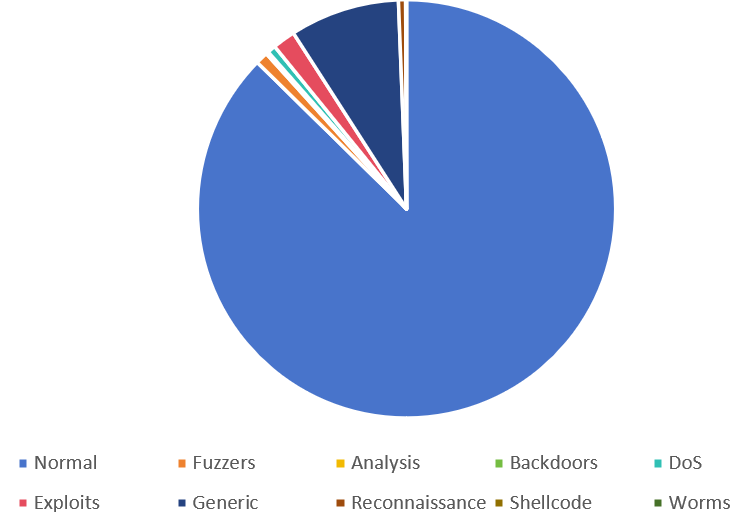
\includegraphics[width = 0.8\textwidth]{UNSW-NB15barchart.png}
	\caption{UNSW-NB15数据集分布占比饼状图}
	\label{fig:UNSW-NB15barchart}
\end{figure}

\begin{table}[htbp]
	\caption{UNSW-NB15数据集中每种攻击的不同子类的细分}
	\label{tab:UNSW-NB15_class}
	\begin{tabularx}{\textwidth}{@{}ccX@{}}
		\toprule
		\multicolumn{1}{c}{\textbf{种类}} & \multicolumn{1}{c}{\textbf{数量}} & \multicolumn{1}{c}{\textbf{子类}}                                                                                                                                                                                                                                                                                                                                                                                                                                                                                                                                   \\
		\multicolumn{1}{c}{\textbf{种类}} & \multicolumn{1}{c}{\textbf{数量}} & \multicolumn{1}{c}{\textbf{子类}}                                                                                                                                                                                                                                                                                                                                                                                                                                                                                                                                   \\
		\midrule
		Fuzzers                           & 10                                & FTP, HTTP, RIP, SMB, Syslog, PPTP, TFTP, DCERPC, OSPF, BGP                                                                                                                                                                                                                                                                                                                                                                                                                                                                                                          \\
		Probe                             & 13                                & Telnet, SNMP, SunRPC Portmapper (TCP) UDP Service, SunRPC Portmapper (TCP) TCP Service, SunRPC Portmapper (UDP) UDP Service, NetBIOS, DNS, HTTP,
		SunRPC Portmapper (UDP), ICMP, SCTP, MSSQL, SMTP                                                                                                                                                                                                                                                                                                                                                                                                                                                                                                                                                                                            \\
		Shellcode                         & 15                                & FreeBSD, HP-UX, NetBSD, AIX, SCO Unix, Linux, Decoders, IRIX, OpenBSD, Mac OS X, BSD, Windows, BSDi, Multiple OS, Solaris                                                                                                                                                                                                                                                                                                                                                                                                                                           \\
		Analysis                          & 3                                 & HTML, Port Scanner, Spam                                                                                                                                                                                                                                                                                                                                                                                                                                                                                                                                            \\
		Backdoors                         & 1                                 & Backdoors                                                                                                                                                                                                                                                                                                                                                                                                                                                                                                                                                           \\
		DoS                               & 36                                & Ethernet, SunRPC, LDAP, Browser, DCERPC, Telnet, NetBIOS/SMB, DNS, TCP, Common Unix Print System (CUPS), Miscellaneous, ISAKMP, Hypervisor,
		Cisco Skinny, IIS Web Server, IGMP, ICMP, XINETD, SIP, RTSP, Windows Explorer, IRC, NTP, CUPS, Asterisk, HTTP, Microsoft Office, SSL, IMAP, SMTP, Oracle, RDP, VNC, FTP, TFTP, SNMP                                                                                                                                                                                                                                                                                                                                                                                                                                                         \\
		Exploits                          & 54                                & Clientside Microsoft Paint, Dameware, Clientside Microsoft Media Player, SSH, SCCP, Unix r Service, SunRPC, LDAP, Web Application, Browser, DCERPC, Interbase, Telnet, DNS, TCP, Webserver, SCADA, SMB, Miscellaneous, Cisco IOS, All, LPD, RADIUS, RDesktop, Unix 'r' Service, IGMP, POP3, ICMP, Clientside Microsoft, Microsoft IIS, Backup Appliance, IDS, Apache, NNTP, RTSP, Evasions, SIP, WINS, Office Document, PHP, Clientside Microsoft Office, Miscellaneous Batch, Browser FTP, MSSQL, SOCKS, PPTP, Clientside, SSL, IMAP, SMTP, Oracle, VNC, FTP, TFTP \\
		Generic                           & 7                                 & All,SIP,HTTP,SMTP,IXIA,TFTP,Superflow                                                                                                                                                                                                                                                                                                                                                                                                                                                                                                                               \\
		Recon                             & 14                                & DNS, HTTP, ICMP, MSSQL, NetBIOS, SCTP, SMTP, SNMP, SunRPC, SunRPC Portmapper (TCP) TCP Service, SunRPC Portmapper (TCP) UDP Service, SunRPC Portmapper (UDP) TCP Service, SunRPC Portmapper (UDP) UDP Service, Telnet                                                                                                                                                                                                                                                                                                                                               \\
		Worms                             & 1                                 & Worms                                                                                                                                                                                                                                                                                                                                                                                                                                                                                                                                                               \\
		Fuzzers                           & 10                                & FTP, HTTP, RIP, SMB, Syslog, PPTP, TFTP, DCERPC, OSPF, BGP                                                                                                                                                                                                                                                                                                                                                                                                                                                                                                          \\
		Probe                             & 13                                & Telnet, SNMP, SunRPC Portmapper (TCP) UDP Service, SunRPC Portmapper (TCP) TCP Service, SunRPC Portmapper (UDP) UDP Service, NetBIOS, DNS, HTTP,
		SunRPC Portmapper (UDP), ICMP, SCTP, MSSQL, SMTP                                                                                                                                                                                                                                                                                                                                                                                                                                                                                                                                                                                            \\
		Shellcode                         & 15                                & FreeBSD, HP-UX, NetBSD, AIX, SCO Unix, Linux, Decoders, IRIX, OpenBSD, Mac OS X, BSD, Windows, BSDi, Multiple OS, Solaris                                                                                                                                                                                                                                                                                                                                                                                                                                           \\
		Analysis                          & 3                                 & HTML, Port Scanner, Spam                                                                                                                                                                                                                                                                                                                                                                                                                                                                                                                                            \\
		Backdoors                         & 1                                 & Backdoors                                                                                                                                                                                                                                                                                                                                                                                                                                                                                                                                                           \\
		DoS                               & 36                                & Ethernet, SunRPC, LDAP, Browser, DCERPC, Telnet, NetBIOS/SMB, DNS, TCP, Common Unix Print System (CUPS), Miscellaneous, ISAKMP, Hypervisor,
		Cisco Skinny, IIS Web Server, IGMP, ICMP, XINETD, SIP, RTSP, Windows Explorer, IRC, NTP, CUPS, Asterisk, HTTP, Microsoft Office, SSL, IMAP, SMTP, Oracle, RDP, VNC, FTP, TFTP, SNMP                                                                                                                                                                                                                                                                                                                                                                                                                                                         \\
		Exploits                          & 54                                & Clientside Microsoft Paint, Dameware, Clientside Microsoft Media Player, SSH, SCCP, Unix r Service, SunRPC, LDAP, Web Application, Browser, DCERPC, Interbase, Telnet, DNS, TCP, Webserver, SCADA, SMB, Miscellaneous, Cisco IOS, All, LPD, RADIUS, RDesktop, Unix 'r' Service, IGMP, POP3, ICMP, Clientside Microsoft, Microsoft IIS, Backup Appliance, IDS, Apache, NNTP, RTSP, Evasions, SIP, WINS, Office Document, PHP, Clientside Microsoft Office, Miscellaneous Batch, Browser FTP, MSSQL, SOCKS, PPTP, Clientside, SSL, IMAP, SMTP, Oracle, VNC, FTP, TFTP \\
		Generic                           & 7                                 & All,SIP,HTTP,SMTP,IXIA,TFTP,Superflow                                                                                                                                                                                                                                                                                                                                                                                                                                                                                                                               \\
		Recon                             & 14                                & DNS, HTTP, ICMP, MSSQL, NetBIOS, SCTP, SMTP, SNMP, SunRPC, SunRPC Portmapper (TCP) TCP Service, SunRPC Portmapper (TCP) UDP Service, SunRPC Portmapper (UDP) TCP Service, SunRPC Portmapper (UDP) UDP Service, Telnet                                                                                                                                                                                                                                                                                                                                               \\
		Worms                             & 1                                 & Worms                                                                                                                                                                                                                                                                                                                                                                                                                                                                                                                                                               \\
		\bottomrule
	\end{tabularx}
\end{table}\par

其次,UNSW-NB15提供了四个CSV格式的数据记录文件,每个文件都包含了攻击记录和正常记录,共2,540,044条记录。
海量的数据集不仅有助于模型的训练和验证,也提高了入侵检测模型在实际环境中应用的可信度和有效性。
此外,UNSW-NB15数据集在设计时注重了实用性和代表性,通过模拟现实世界的网络环境和流量模式,确保了数据集的广泛适用性和长期价值。
这使得该数据集成为评估和比较不同入侵检测技术性能的理想选择。\par

\textbf{2.实验环境}\par
为了评估本文所提方案的有效性,本文将利用python语言来实现以上流程,并选用表~\ref{tab:env_setting}~中的配置来进行实验。
\begin{table}[htbp]
	\caption{实验设备配置}
	\label{tab:env_setting}
	\centering
	\begin{tabular}{ccc}
		\toprule
		\textbf{环境类别}         & \textbf{设备项目} & \textbf{项目参数}                  \\
		\textbf{环境类别}         & \textbf{设备项目} & \textbf{项目参数}                  \\
		\midrule
		\multirow{6}{*}{硬件环境} & CPU型号           & Intel(R) Core(TM) i7-11800H        \\
		                          & CPU规格           & 8核16线程@2.30GHz                  \\
		                          & GPU型号           & NVIDIA GeForce RTX 3060 Laptop GPU \\
		                          & 内存大小          & 16.0 GB                            \\
		                          & 硬盘类型          & SSD                                \\
		                          & 硬盘大小          & 1TB                                \\
		\multirow{6}{*}{硬件环境} & CPU型号           & Intel(R) Core(TM) i7-11800H        \\
		                          & CPU规格           & 8核16线程@2.30GHz                  \\
		                          & GPU型号           & NVIDIA GeForce RTX 3060 Laptop GPU \\
		                          & 内存大小          & 16.0 GB                            \\
		                          & 硬盘类型          & SSD                                \\
		                          & 硬盘大小          & 1TB                                \\
		\hline
		\multirow{3}{*}{软件环境} & 操作系统          & Windows 11                         \\
		                          & 开发语言          & Python 3.11.7                      \\
		                          & 编辑器            & Visual Studio Code                 \\
		                          & 开发语言          & Python 3.11.7                      \\
		                          & 编辑器            & Visual Studio Code                 \\
		\bottomrule
	\end{tabular}
\end{table}

\textbf{3.评估指标}\par
本文主要使用准确度 (Accuracy)、精确度 (Precision)、召回率 (Recall)、加权平均 F1 分数 (Macro Averaged F1 Score)、宏平均 F1 分数 (Macro Averaged F1 Score)这5个评价指标对我们的方案进行全方位的评估。
以下是这5个指标的简单介绍。\par
1)~准确度\par
表示模型正确预测的比例,是所有正确预测的数量除以总预测数量。
\begin{equation}
	\label{eq:val_score1}
	Accuracy = \frac{Number of Correct Predictions}{Total Number of Predictions} = \frac{TP + TN}{TP + TN + FP + FN}
\end{equation}

2)~精确度\par
简称精度,也称为查准率,是所有模型预测为正类的样本中,实际为正类的比例。
\begin{equation}
	\label{eq:val_score2}
	Precision = \frac{TP}{TP + FP}
\end{equation}

3)~召回率\par
召回率,也称为真正率、查补率,是模型正确识别为正类的样本占所有实际正类样本的比例。
\begin{equation}
	\label{eq:val_score3}
	Recall = \frac{TP}{TP + FN}
\end{equation}

4)~宏平均~F1~分数\par
宏平均~F1~分数是一种性能评估指标,用于衡量模型在所有类别上的平均表现。
它通过简单地计算所有类别~F1~分数的算术平均值得出,每个类别被赋予相同的权重,不论其样本量大小。
\begin{equation}
	\label{eq:val_score4}
	F1_{macro} = \frac{1}{N} \sum\limits_{i=1}^{N} F1_i
\end{equation}
\begin{flushleft}
	\renewcommand\arraystretch{1.25}
	\begin{tabularx}{\textwidth}{@{}>{\normalsize\rm}l@{\quad}>{\normalsize\rm}l@{——}>{\normalsize\rm}X@{}}
		式中 & $F1_{macro}$ & 表示宏平均 F1 分数;          \\
		     & $N$          & 类别总数;                    \\
		     & $F1_i$       & 表示第 $i$ 个类别的 F1 分数。 \\
	\end{tabularx}\vspace{.5ex}
		式中 & $F1_{macro}$ & 表示宏平均 F1 分数;          \\
		     & $N$          & 类别总数;                    \\
		     & $F1_i$       & 表示第 $i$ 个类别的 F1 分数。 \\
	\end{tabularx}\vspace{.5ex}
\end{flushleft}
宏平均 F1 分数特别适用于样本分布不均匀的数据集,因为它给每个类别分配了同等的重要性。
这样做确保了即使某些类别的样本数量很少,它们在计算平均分数时也会有相等的影响。\par

5)~加权平均 F1 分数\par
加权平均F1分数是一种性能评估指标,通过根据每个类别的样本量对其F1分数进行加权平均,以反映所有类别的整体性能。
每个类别的重要性通过其在数据集中的相对比例来确定。
\begin{equation}
	\label{eq:val_score5}
	F1_{weighted} = \sum\limits_{i=1}^{N} w_i \cdot F1_i
\end{equation}
\begin{flushleft}
	\renewcommand\arraystretch{1.25}
	\begin{tabularx}{\textwidth}{@{}>{\normalsize\rm}l@{\quad}>{\normalsize\rm}l@{——}>{\normalsize\rm}X@{}}
		式中 & $F1_{weighted}$ & 加权平均F1分数;                                                  \\
		     & $N$             & 类别总数;                                                        \\
		     & $F1_i$          & 第$i$个类别的F1分数                                               \\
		     & $w_i$           & 第$i$个类别的权重,通常由该类别的样本数量占总样本数量的比例确定。 \\
	\end{tabularx}\vspace{.5ex}
		式中 & $F1_{weighted}$ & 加权平均F1分数;                                                  \\
		     & $N$             & 类别总数;                                                        \\
		     & $F1_i$          & 第$i$个类别的F1分数                                               \\
		     & $w_i$           & 第$i$个类别的权重,通常由该类别的样本数量占总样本数量的比例确定。 \\
	\end{tabularx}\vspace{.5ex}
\end{flushleft}

上式\ref{eq:val_score1}、\ref{eq:val_score2}、\ref{eq:val_score3}%、\ref{eq:val_score4}、\ref{eq:val_score5}\ref{eq:val_score6}、\ref{eq:val_score7}%
中,
$TP$(True Positives)表示正确地将正类预测为正类;
$TN$(True Negatives)表示正确地将负类预测为负类;
$FP$(False Positives)表示错误地将负类预测为正类;
$FN$(False Negatives)表示错误地将正类预测为负类。

\textbf{4.特征编码效果实验评估}\par
在本次实验中,我们通过比较特征编码前后各种机器学习和深度学习模型的准确率(如表~\ref{tab:model_performance}~以及图~\ref{fig:comapre_accuracy_encoding}~所示,
\begin{figure}[htbp]
	\centering
	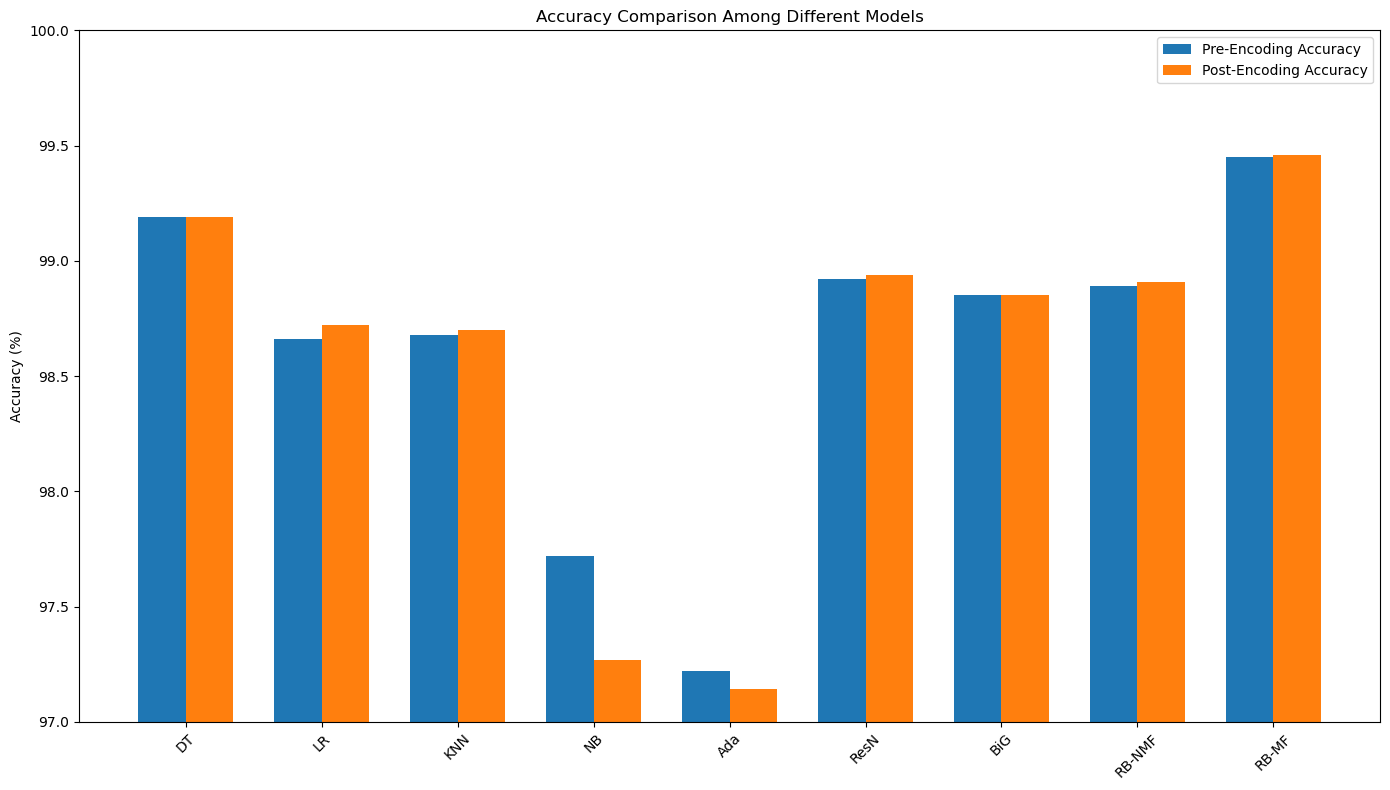
\includegraphics[width = \textwidth]{acc.png}
	\caption{特征编码前后模型预测准确率对比条状图}
	\label{fig:comapre_accuracy_encoding}
\end{figure}
\begin{table}[htbp]
	\centering
	\setlength{\tabcolsep}{1pt}
	\setlength{\tabcolsep}{1pt}
	\caption{特征编码前后模型表现}
	\label{tab:model_performance}
	\begin{tabular}{cccccccccc}
	\begin{tabular}{cccccccccc}
		\toprule
		        & DT               & LR              & KNN             & NB             & Ada               & ResN            & BiG           & RB-NMF          & RB-MF           \\
		        & DT               & LR              & KNN             & NB             & Ada               & ResN            & BiG           & RB-NMF          & RB-MF           \\
		\midrule
		\multicolumn{9}{c}{\textbf{特征编码前}}                                                                                                                                   \\
		Acc     & 99.19\%          & 98.66\%         & 98.68\%         & 97.72\%        & 97.22\%           & 98.92\%         & 98.85\%       & 98.89\%         & 99.45\%         \\
		f1\_mac & 0.5422           & 0.3730          & 0.4042          & 0.3376         & 0.3609            & 0.4110          & 0.493         & 0.518           & 0.529           \\
		f1\_wei & 0.9925           & 0.9874          & 0.9872          & 0.9726         & 0.9704            & 0.9892          & 0.9885        & 0.9891          & 0.9945          \\
		\multicolumn{9}{c}{\textbf{特征编码前}}                                                                                                                                   \\
		Acc     & 99.19\%          & 98.66\%         & 98.68\%         & 97.72\%        & 97.22\%           & 98.92\%         & 98.85\%       & 98.89\%         & 99.45\%         \\
		f1\_mac & 0.5422           & 0.3730          & 0.4042          & 0.3376         & 0.3609            & 0.4110          & 0.493         & 0.518           & 0.529           \\
		f1\_wei & 0.9925           & 0.9874          & 0.9872          & 0.9726         & 0.9704            & 0.9892          & 0.9885        & 0.9891          & 0.9945          \\
		\midrule
		\multicolumn{9}{c}{\textbf{特征编码后}}                                                                                                                                   \\
		Acc     & 99.19\%          & 98.72\%\uparrow & 98.70\%\uparrow & 97.27\%        & 97.14\%\downarrow & 98.94\%\uparrow & 98.85\%       & 98.91\%\uparrow & 99.46\%\uparrow \\
		f1\_mac & 0.5378\downarrow & 0.3871\uparrow  & 0.4090\uparrow  & 0.2166         & 0.3197\downarrow  & 0.4166\uparrow  & 0.495\uparrow & 0.52\uparrow    & 0.53\uparrow    \\
		f1\_wei & 0.9925           & 0.9879\uparrow  & 0.9873\uparrow  & 0.9729\uparrow & 0.9723\uparrow    & 0.9898\uparrow  & 0.9885        & 0.9892\uparrow  & 0.9946\uparrow  \\
		\multicolumn{9}{c}{\textbf{特征编码后}}                                                                                                                                   \\
		Acc     & 99.19\%          & 98.72\%\uparrow & 98.70\%\uparrow & 97.27\%        & 97.14\%\downarrow & 98.94\%\uparrow & 98.85\%       & 98.91\%\uparrow & 99.46\%\uparrow \\
		f1\_mac & 0.5378\downarrow & 0.3871\uparrow  & 0.4090\uparrow  & 0.2166         & 0.3197\downarrow  & 0.4166\uparrow  & 0.495\uparrow & 0.52\uparrow    & 0.53\uparrow    \\
		f1\_wei & 0.9925           & 0.9879\uparrow  & 0.9873\uparrow  & 0.9729\uparrow & 0.9723\uparrow    & 0.9898\uparrow  & 0.9885        & 0.9892\uparrow  & 0.9946\uparrow  \\
		\bottomrule
	\end{tabular}
\end{table}
其中DT、LR、KNN、 NB、 Ada、ResN、BiG、RB-NMF、RB-MF分别代表决策树、逻辑回归、K近邻、朴素贝叶斯、Ada增强、残差神经网络、双向门控循环单元、未经过多模态特征融合的残差神经网络与门控循环单元混合模型以及经过多模态特征融合的残差神经网络与门控循环单元混合模型),得出了一些发现。
首先,决策树模型在应对输入数据表示形式的变化时,表现出卓越的鲁棒性,其准确率在特征编码前后基本保持不变。
相比之下,逻辑回归和K近邻等模型在特征编码后轻微提升了准确率,这表明特征编码可能会对这些模型带来微小的性能提升。
然而,朴素贝叶斯模型在特征编码后的准确率却出现显著的下降。
这主要是由于特征编码改变了数据的原始分布假设,从而对基于概率的朴素贝叶斯模型产生较大的影响。
在深度学习领域,ResNet和BiGRU模型在特征编码后准确率则得到稳定提升。
这主要归功于这些模型能够从编码后的特征中学习到更为复杂和深层的数据表示。
特别值得一提的是,采用多模态特征融合的ResNet-BiGRU模型在特征编码前后准确率均最高。
尤其在特征编码后,其准确率更是高达99.46\%,这充分凸显了模态融合在提升模型处理能力方面的显著优势。\par


整体而言,所有模型在准确率方面都表现出较高的水平,特别是在特征编码后,大多数模型的准确率略有提升,说明特征编码对模型性能有正面影响。
具体到F1分数,F1 Macro(图~\ref{fig:f1_macro_score}~)和F1 Weighted(图~\ref{fig:f1_weighted_score}~)分数在特征编码后也显示出类似的趋势。
\begin{figure}[htbp]
	\centering
	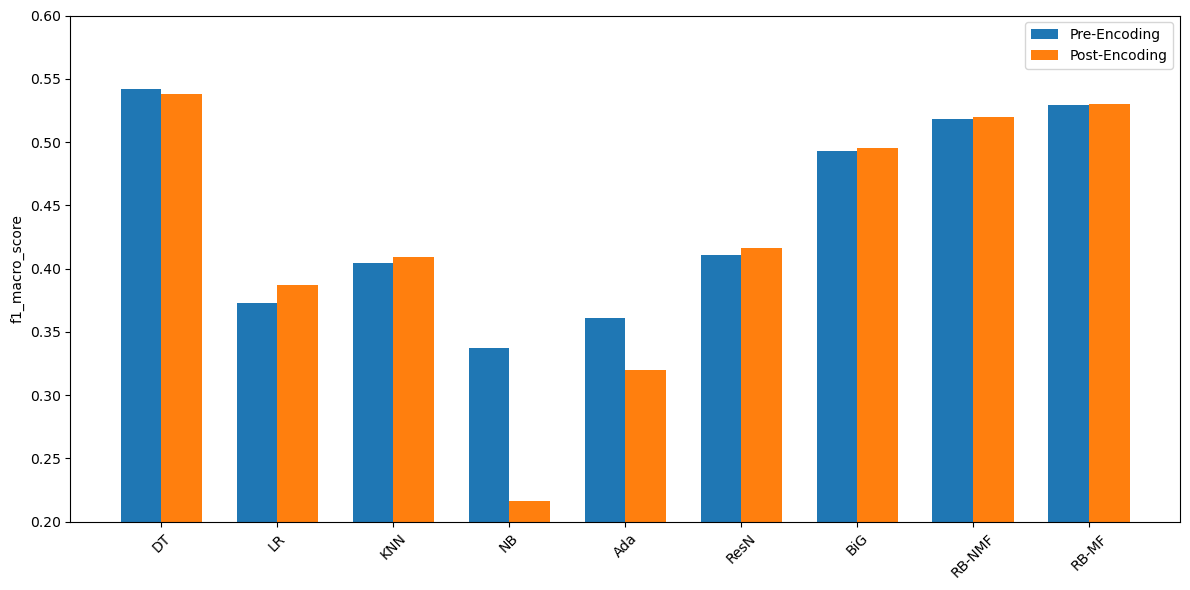
\includegraphics[width = \textwidth]{f1-mac.png}
	\caption{特征编码前后模型f1 macro score对比条状图}
	\label{fig:f1_macro_score}
\end{figure}
\begin{figure}[htbp]
	\centering
	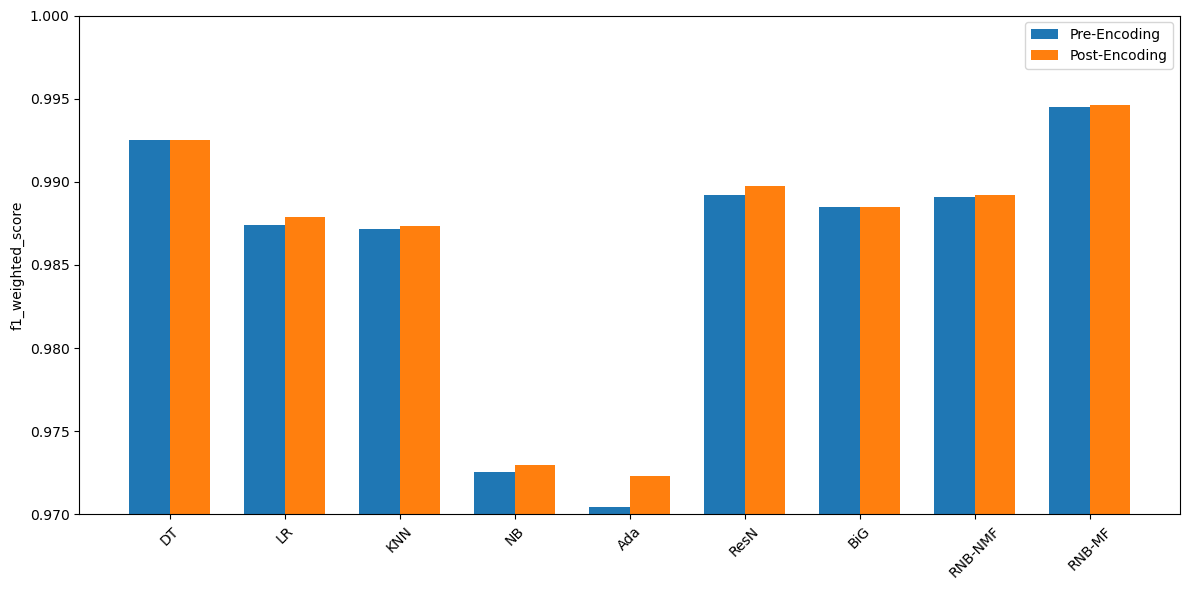
\includegraphics[width = \textwidth]{f1-wei.png}
	\caption{特征编码前后模型f1 weighted score对比条状图}
	\label{fig:f1_weighted_score}
\end{figure}
在深度学习模型方面,ResNet和BiGRU表现出了较好的性能提升,尤其是在特征编码后,这主要归因于深度学习模型能够从编码后的特征中学习到更加复杂的表示。
同样值得注意的是,采用模态融合策略的ResNet-BiGRU模型在所有评价指标上都表现最优,无论是在特征编码前还是编码后。
经过对数据的细致分析后,我们可以看到特征编码和模型选择对于提升模型性能具有重要意义。
模态特征融合技术尤其在提高复杂模型的准确率和F1分数方面显示出显著的优势,这为未来模型设计和特征工程方面的研究提供了有价值的参考。\par

\textbf{5.数据集平衡处理效果实验评估}\par
在处理网络流量数据时,一个常见的挑战是数据的不平衡性。特别是在网络安全领域,正常流量的样本远多于异常或攻击流量的样本。
例如,在本章所使用的数据集中,正常流量样本占据了总样本的87\%,因此,即使模型简单地将所有流量都判断为正常流量,其准确率依然能够达到87\%。
然而,这种“一刀切”的模型在异常流量检测任务中毫无效果,因为它无法识别出任何异常样本。\par

为了解决这一问题,本文将采用SMOTE算法对异常样本进行过采样处理。
通过这种方法,我们能够增加异常流量样本的数量,从而改善训练数据的平衡性。
过采样的结果如表~\ref{tab:attack_num_transposed_part1}~所示,
\begin{table}[h]
	\centering
	\caption{数据集平衡处理前后数据量变化}
	\label{tab:attack_num_transposed_part1}
	\begin{tabular}{cccccc}
		\toprule
		攻击种类          & \textbf{Fuzzers} & \textbf{Analysis} & \textbf{Backdoors} & \textbf{DoS} & \textbf{Exploits} \\
		\midrule
		\textbf{过采样前} & 3775             & 382               & 400                & 879          & 4038              \\
		\textbf{过采样后} & 50844            & 50844             & 50844              & 50844        & 50844             \\
		\bottomrule
	\end{tabular}
	\begin{tabular}{ccccc}
		\toprule
		攻击种类          & \textbf{Generic} & \textbf{Recon} & \textbf{Shellcode} & \textbf{Worms} \\
		\midrule
		\textbf{过采样前} & 5587             & 1316           & 164                & 18             \\
		\textbf{过采样后} & 50844            & 50844          & 50844              & 50844          \\
		\bottomrule
	\end{tabular}
\end{table}
从中可以看出,过采样后各类样本的数量有了明显的变化。
此外,本文使用PCA(主成分分析)方法将样本降维到了2D平面上,并在图~\ref{fig:prepostsmote}中展示了过采样前后的情况。
\begin{figure}[htbp]
	\centering
	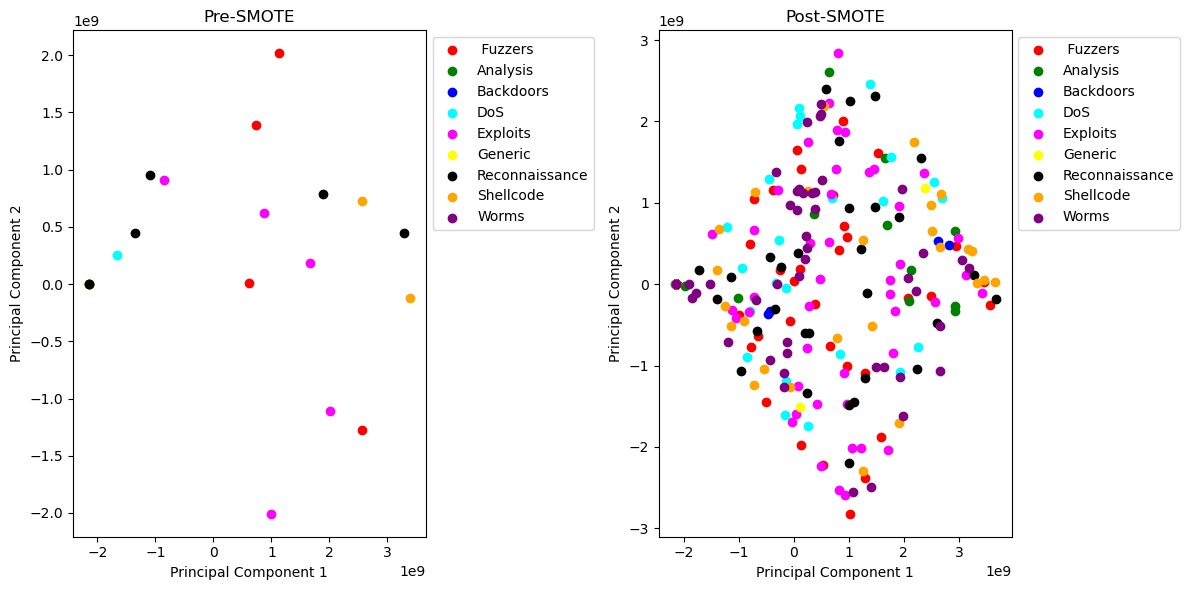
\includegraphics[width = 0.8 \textwidth]{smote.png}
	\caption{SMOTE过采样前后,1000个样本中各种攻击类别的样本点变化,这里省略了normal样本点}
	\label{fig:prepostsmote}
\end{figure}
从图中可以看到,攻击样本的数量在过采样后有了显著的增加,这有助于模型学习到更加均衡的数据表示。\par

最终,本文评估了过采样对模型性能的影响。
表~\ref{tab:model_performance_oversampling}~展示了过采样前后各类样本检测的召回率变化。
\begin{table}[htbp]
	\centering
	\caption{过采样前后各种攻击检测召回率变化}
	\label{tab:model_performance_oversampling}
	\begin{tabular}{cccccccccc}
		\toprule
		          & DT    & LR    & KNN   & NB    & Ada   & ResN  & BiG   & RB-NMF & RB-MF \\
		\midrule
		\multicolumn{10}{c}{\textbf{过采样前}}                                             \\
		\multicolumn{10}{c}{\textbf{过采样前}}                                             \\
		Fuzzers   & 0.825 & 0.624 & 0.614 & 0.019 & 0.064 & 0.713 & 0.709 & 0.699  & 0.842 \\
		Analysis  & 0.115 & 0     & 0     & 0.566 & 0.844 & 0     & 0     & 0      & 0.361 \\
		Backdoors & 0     & 0     & 0     & 0     & 0.059 & 0     & 0     & 0      & 0.288 \\
		DoS       & 0.165 & 0.051 & 0.114 & 0.008 & 0     & 0.017 & 0.322 & 0.341  & 0.458 \\
		Exploits  & 0.666 & 0.705 & 0.639 & 0.04  & 0.001 & 0.808 & 0.716 & 0.796  & 0.796 \\
		Generic   & 0.962 & 0.925 & 0.931 & 0.956 & 0.921 & 0.935 & 0.876 & 0.899  & 0.943 \\
		Recon     & 0.91  & 0.755 & 0.58  & 0.019 & 0.854 & 0.739 & 0.743 & 0.757  & 0.946 \\
		Shellcode & 0.66  & 0     & 0.14  & 0.98  & 0.76  & 0.067 & 0.045 & 0.073  & 0.937 \\
		Worms     & 0     & 0     & 0     & 0.75  & 0     & 0     & 0     & 0      & 0     \\
		normal    & 1     & 0.997 & 0.997 & 0.993 & 0.99  & 0.998 & 0.999 & 0.999  & 0.999 \\
		\midrule
		\multicolumn{10}{c}{\textbf{过采样后}}                                             \\
		\multicolumn{10}{c}{\textbf{过采样后}}                                             \\
		Fuzzers   & 0.838 & 0.041 & 0.701 & 0.099 & 0.606 & 0.723 & 0.714 & 0.703  & 0.857 \\
		Analysis  & 0.452 & 0.032 & 0.565 & 0     & 0     & 0.013 & 0     & 0      & 0.564 \\
		Backdoors & 0.362 & 0.31  & 0.431 & 0.931 & 0.948 & 0     & 0     & 0      & 0.412 \\
		DoS       & 0.521 & 0     & 0.479 & 0.009 & 0     & 0.023 & 0.125 & 0.16   & 0.634 \\
		Exploits  & 0.807 & 0     & 0.659 & 0.026 & 0     & 0.809 & 0.714 & 0.806  & 0.822 \\
		Generic   & 0.992 & 0.187 & 0.948 & 0     & 0.926 & 0.941 & 0.875 & 0.893  & 0.941 \\
		Recon     & 0.995 & 0     & 0.872 & 0.511 & 0     & 0.724 & 0.742 & 0.759  & 0.933 \\
		Shellcode & 1     & 0     & 0.933 & 0.133 & 0.867 & 0.132 & 0.044 & 0.081  & 0.961 \\
		Worms     & 1     & 0     & 1     & 0     & 1     & 0     & 0     & 0      & 0     \\
		normal    & 1     & 0.99  & 0.97  & 0.624 & 0.985 & 0.996 & 0.999 & 0.999  & 0.999 \\
		\bottomrule
	\end{tabular}
\end{table}
通过分析该表格可知,过采样后,绝大多数模型在检测各类攻击事件时的召回率有了显著提高。
尤其是对于那些原本难以被检测到的攻击类型,如Backdoors、Analysis等,过采样为这些攻击类型提供了更多的样本,使得模型能够学习到更加丰富的特征,从而在这些攻击类型上获得了更好的召回率。\par

表~\ref{tab:oversampling_performance}~则展示了过采样前后各类样本检测精确度的变化。
\begin{table}[htbp]
	\centering
	\caption{过采样前后各种攻击检测精度变化}
	\label{tab:oversampling_performance}
	\begin{tabular}{lccccccccc}
		\toprule
		          & DT    & LR    & KNN   & NB    & Ada   & ResN  & BiG   & RB-NMF & RB-MF \\
		\midrule
		\multicolumn{10}{c}{\textbf{过采样前}}                                             \\
		\multicolumn{10}{c}{\textbf{过采样前}}                                             \\
		Fuzzers   & 0.659 & 0.455 & 0.497 & 0.667 & 0.545 & 0.542 & 0.534 & 0.536  & 0.697 \\
		Analysis  & 1     & 0     & 0     & 0.117 & 0.054 & 0     & 0     & 0      & 0.201 \\
		Backdoors & 0.0   & 0.0   & 0     & 0     & 0.092 & 0     & 0     & 0      & 0     \\
		DoS       & 0.255 & 0.279 & 0.206 & 0.222 & 0.0   & 0.250 & 0.23  & 0.17   & 0.27  \\
		Exploits  & 0.662 & 0.623 & 0.649 & 0.763 & 0.200 & 0.620 & 0.411 & 0.656  & 0.686 \\
		Generic   & 0.966 & 0.988 & 0.983 & 0.589 & 0.997 & 0.966 & 0.746 & 0.826  & 0.979 \\
		Recon     & 0.894 & 0.562 & 0.567 & 0.019 & 0.320 & 0.747 & 0.743 & 0.863  & 0.905 \\
		Shellcode & 0.767 & 0.0   & 0.538 & 0.04  & 0.365 & 1     & 0.665 & 0.665  & 0.732 \\
		Worms     & 0.0   & 0     & 0     & 0.009 & 0     & 0     & 0     & 0      & 0     \\
		normal    & 1     & 0.998 & 0.997 & 0.998 & 0.99  & 0.998 & 0.999 & 0.999  & 0.999 \\
		\midrule
		\multicolumn{10}{c}{\textbf{过采样后}}                                             \\
		\multicolumn{10}{c}{\textbf{过采样后}}                                             \\
		Fuzzers   & 0.756 & 0.22  & 0.409 & 0.427 & 0.465 & 0.566 & 0.512 & 0.536  & 0.772 \\
		Analysis  & 0.065 & 0.037 & 0.147 & 0     & 0     & 0.052 & 0     & 0      & 0.253 \\
		Backdoors & 0.053 & 0.032 & 0.135 & 0.011 & 0.140 & 0.013 & 0.112 & 0      & 0     \\
		DoS       & 0.17  & 0     & 0.162 & 0.002 & 0     & 0.102 & 0.24  & 0.205  & 0.24  \\
		Exploits  & 0.762 & 0     & 0.458 & 0.412 & 0     & 0.505 & 0.311 & 0.493  & 0.801 \\
		Generic   & 0.973 & 0.274 & 0.972 & 0     & 0.996 & 0.921 & 0.446 & 0.801  & 0.978 \\
		Recon     & 0.889 & 0     & 0.333 & 0.007 & 0     & 0.355 & 0.636 & 0.799  & 0.884 \\
		Shellcode & 0.793 & 0     & 0.108 & 0.035 & 0.28  & 0.204 & 0.541 & 0.637  & 0.774 \\
		Worms     & 0     & 0     & 0.004 & 0     & 0.002 & 0     & 0     & 0      & 0     \\
		normal    & 0.999 & 0.976 & 0.999 & 0.999 & 0.995 & 0.996 & 0.999 & 0.999  & 0.999 \\
		\bottomrule
	\end{tabular}
\end{table}
在检测精度方面,虽然过采样导致某些模型在个别攻击类型上的精度有所下降,这主要是因为引入了更多的少数类样本。
为了提高对这些少数类的识别准确率,模型可能会在一定程度上牺牲对多数类的识别精度。
然而,从整体上看,模型的总体性能是得到了改善的。\par

另外,RB-MF(表中的RB-MF),即经过模态融合的残差网络和双向门控循环单元的混合模型,表现出了卓越的性能。
过采样后,几乎所有攻击类型的召回率均有所提高,同时精度在大多数情况下也得以保持甚至略有提升。
这说明RB-MF模型能够有效利用过采样带来的额外信息,而且模态融合策略提高了模型处理不平衡数据的能力,使其在面对复杂的攻击检测任务时,能够更加准确地识别出少数类攻击样本,同时保持对正常流量的高识别精度。\par


图~\ref{fig:ResNet-BiGRU-NoFusion-loss}~、~\ref{fig:ResNet-BiGRU-Fusion-loss}~分别是RB-NMF以及RB-MF各epoch的损失曲线以及准确率曲线。
\begin{figure}[htbp]
	\centering
	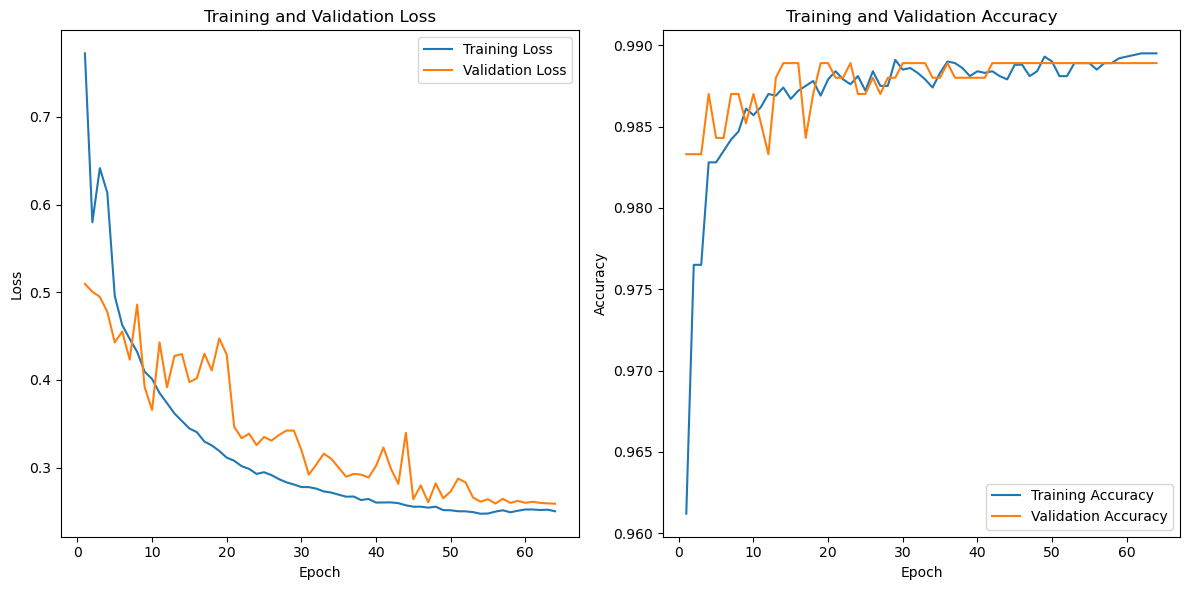
\includegraphics[width = \textwidth]{resnet_bigure_nmf.png}
	\caption{RB-NMF各epoch的损失曲线以及准确率曲线}
	\label{fig:ResNet-BiGRU-NoFusion-loss}
\end{figure}
\begin{figure}[htbp]
	\centering
	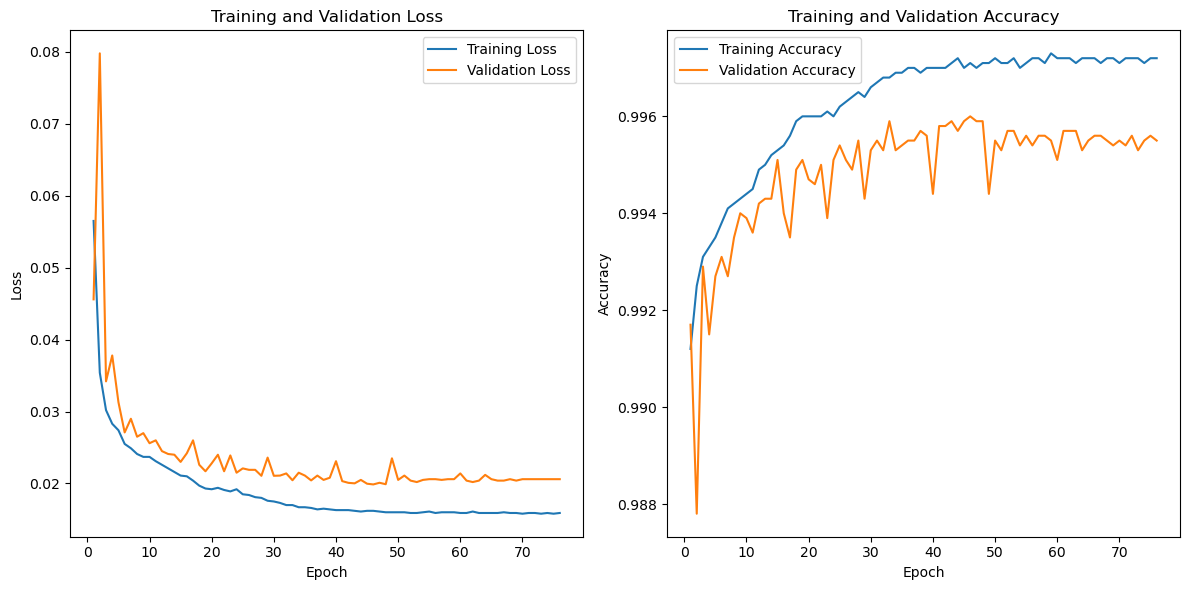
\includegraphics[width = \textwidth]{resnet_bigure_curve.png}
	\caption{RB-MF各epoch的损失曲线以及准确率曲线}
	\label{fig:ResNet-BiGRU-Fusion-loss}
\end{figure}
通过观察损失函数图表可知,未经模态融合的模型训练和验证损失都在逐渐减小,但验证损失的波动较大,这可能表明模型在训练集上有过拟合的趋势。
相比之下,经过模态融合的模型损失下降更为平滑,且在训练后期,验证损失几乎与训练损失保持一致,这表明模型具有更好的泛化能力。\par
虽然未经模态融合的模型在初期展现出了相对较高的准确率,但在训练过程中,其性能出现了明显的波动,特别是在验证准确率方面,出现这一现象的原因极有可能是模型存在过拟合问题。
相比之下,经过模态融合的模型不仅在训练初期就迅速提升了准确率,而且在后续的训练过程中也持续保持在非常高的水平,几乎没有任何波动。
这一结果充分体现了本文所设计的模型强大的稳定性和预测准确率。\par

\section{基于特征融合模型的增量学习方案}
在前几个小节中,我们已经通过实验验证了RB-MF模型在网络攻击检测任务上的性能优势。
具体而言,此模型针对UNSW-NB15数据集中的网络流量数据展现出了卓越的处理效果。
然而,值得注意的是,该模型的应用范围会受到其训练数据集独特性质的制约。
这意味着,当面对与UNSW-NB15数据集具有显著不同的新数据时,模型的表现可能会受到一定的影响。
例如,随着时间推移,新数据的不断累积使得模型需不断适应新增的信息,而旧数据可能因存储限制或隐私保护政策等因素而逐渐失去可用性。
此外,学习任务的复杂度亦可能随之增加,如分类任务中类别数的增长等,而这些变化往往无法事先预定义。\par

因此,探索如何有效地使模型适应新类型的数据,以及如何在数据动态变化的情境下保持模型的稳定性和准确性,成为了重要的研究课题。
针对这一问题,增量学习(Incremental Learning)的概念便成为解决上述问题的一个有效途径。
增量学习(图~\ref{fig:incremental_learning}~所示)旨在使模型能够逐渐适应新数据或新任务,而无需从头开始重新训练模型。
\begin{figure}[htbp]
	\centering
	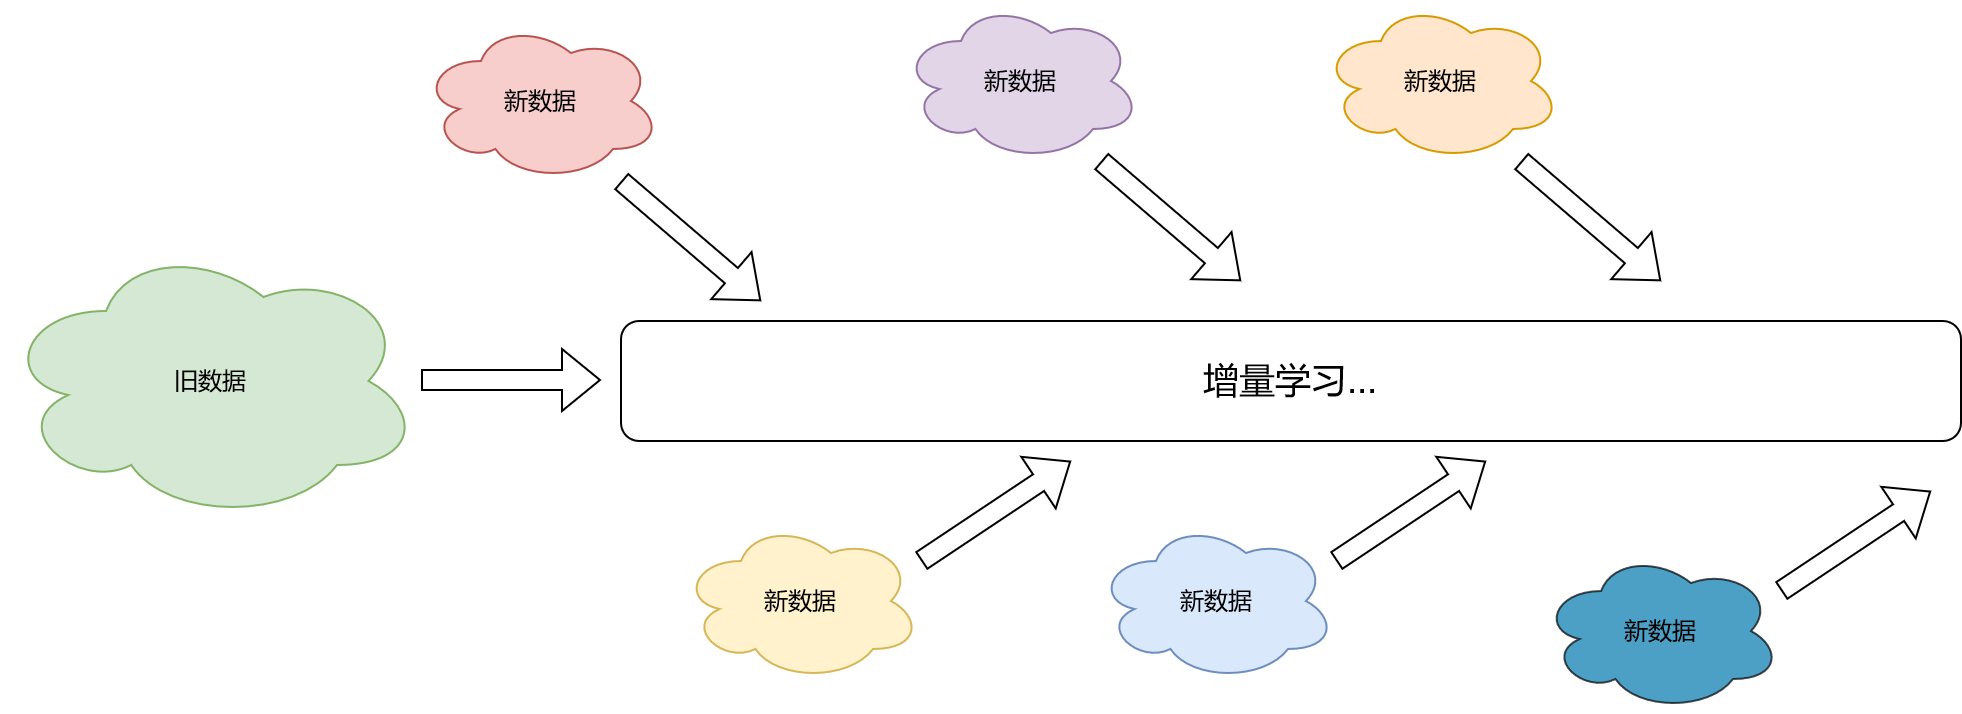
\includegraphics[width=0.9\textwidth]{increment_learning.drawio.png}
	\caption{增量学习原理图}
	\label{fig:incremental_learning}
\end{figure}
具体而言,增量学习允许模型在保留已学习知识的基础上,持续地吸收新信息并更新其知识库。

\subsection{方案具体设计}
iCaRL(Incremental Classifier and Representation Learning)\cite{rebuffi2017icarl}是一种经典的基于回放的增量学习策略。
基于回放的增量学习的基本思想就是"温故而知新",即在接受新任务的训练过程中,同时回顾一部分精选的旧数据,以此来保持模型对先前学习任务的记忆。
因此,决定保留哪些旧任务数据以及如何有效地结合旧数据和新数据进行模型训练,是这类方法需要考虑的主要问题。\par

iCaRL的一般步骤为数据特征的学习、记忆集的管理,以及通过知识蒸馏减轻模型的遗忘。
当面对新的数据批次时,iCaRL首先结合这些新数据和从记忆集中选出的代表性样本来更新模型。
记忆集是由每个已知类别中挑选出的一小部分样本构成,旨在代表整个类别的特征分布。
通过在训练过程中包含这些样本,模型可以重新回顾已学习的类别,从而在学习新知识的同时,尽量减少对旧知识的遗忘。
接着,iCaRL通过一个更新的特征提取器来获取数据的特征表示,并利用这些特征来进行分类学习。
在学习新类别的同时,iCaRL使用知识蒸馏来保持对过去学习内容的记忆。
通过将旧模型对同一数据的输出作为额外的训练目标,新模型能够在吸收新信息的同时,减少对旧信息的遗忘。
分类决策在iCaRL中是通过计算样本与每个类别的代表性样本(即记忆集中的样本)的平均特征向量(即类中心见公式\ref{eq:class_means})之间的距离来进行的。
\begin{equation}
	\label{eq:class_means}
	\mu_c = \frac{1}{|P_c|} \sum_{p \in P_c} f(p)
\end{equation}
\begin{flushleft}
	\renewcommand\arraystretch{1.25}
	\begin{tabularx}{\textwidth}{@{}>{\normalsize\rm}l@{\quad}>{\normalsize\rm}l@{——}>{\normalsize\rm}X@{}}
		式中 & $P_c$  & 表示类别$c$的样本集; \\
		     & $f(p)$ & 样本$p$的特征表示。   \\
	\end{tabularx}\vspace{.5ex}
		     & $f(p)$ & 样本$p$的特征表示。   \\
	\end{tabularx}\vspace{.5ex}
\end{flushleft}
分类决策的公式如式~\ref{eq:class_dist}~所示。
\begin{equation}
	\label{eq:class_dist}
	\hat{y} = \arg\min_{c \in C} \|f(x) - \mu_c\|_2
\end{equation}
\begin{flushleft}
	\renewcommand\arraystretch{1.25}
	\begin{tabularx}{\textwidth}{@{}>{\normalsize\rm}l@{\quad}>{\normalsize\rm}l@{——}>{\normalsize\rm}X@{}}
		式中 & $\hat{y}$          & 表示预测的类别;                                  \\
		     & $|f(x) - \mu_c|_2$ & 测试样本特征表示与类别$c$的类中心之间的欧氏距离。 \\
	\end{tabularx}\vspace{.5ex}
		式中 & $\hat{y}$          & 表示预测的类别;                                  \\
		     & $|f(x) - \mu_c|_2$ & 测试样本特征表示与类别$c$的类中心之间的欧氏距离。 \\
	\end{tabularx}\vspace{.5ex}
\end{flushleft}
这种基于最近中心的方法简单有效,因为它直接使用了模型学习到的特征表示来进行类别的判断。

最后,更新记忆集是iCaRL算法中一个至关重要的步骤。
随着新类别的加入,算法必须在有限的记忆容量中做出取舍,选择哪些样本继续保留在记忆集中。
这通常会涉及到对每个类别进行均衡的考虑,确保模型能够公平地回顾所有已知类别,而不是偏向于某些特定的类别。\par

基于此策略,本文接下来会将提出的RB-MF模型整合到iCaRL框架中,进而赋予其增量学习的能力。
融合RB-MF模型的iCaRL策略实现伪代码如表~\ref{tab:RB-MF-icarl}~所示。
\begin{table}[htbp]
	\caption{融合RB-MF模型的iCaRL}
	\label{tab:RB-MF-icarl}
	\centering
	\begin{tabularx}{1.0\textwidth}{cl}
		\toprule
		\multicolumn{2}{l}{\textbf{融合RB-MF模型的iCaRL策略实现}}                                                    \\
		\midrule
		\multicolumn{2}{l}{\textbf{输入}: 训练序列中的一系列数据集 $\{D_1, D_2, ..., D_n\}$,每个类别保留的样本数 $m$} \\
		\multicolumn{2}{l}{\textbf{输出}: 训练好的RB-MF特征提取器 $f_{\theta}$,更新后的记忆集 $M$}                  \\
		1  & 初始化记忆集 $M$ 为空                                                                                     \\
		2  & 初始化RB-MF特征提取器 $f_{\theta}$                                                                      \\
		3  & $for$ 每个新的数据集 $D_t$:                                                                               \\
		4  & \quad\quad $D'_t = D_t \cup M$     \Comment{合并新任务数据集和记忆集}                                     \\
		5  & \quad\quad 如果 $t > 1$,即不是处理第一个数据集:                                                          \\
		6  & \quad\quad\quad\quad 使用$f_{\theta}$的旧版本对$x$进行前向传播,得到旧类别的输出$logits_{old}$            \\
		7  & \quad\quad\quad\quad 使用知识蒸馏损失和分类损失来更新 $f_{\theta}$:                                       \\
		8  & \quad\quad\quad\quad\quad\quad $L = (1 - \alpha) L_{CE} + \alpha L_{KD}$                                  \\ %\Comment{L:整体损失,$L_{CE}$:蒸馏损失,$L_{KD}$:标准交叉熵损失} 
		9  & \quad\quad 否则,如果是处理第一个数据集:                                                                  \\
		10 & \quad\quad\quad\quad 仅使用分类损失来训练 $f_{\theta}$                                                    \\
		11 & \quad\quad $for$ 每个类别 $c=1$ 到 $n$:                                                                   \\
		12 & \quad\quad\quad\quad 从属于类别$c$的数据集$D_c$中提取所有样本$\{x_1, x_2, ..., x_k\}$                     \\
		13 & \quad\quad\quad\quad 使用当前的特征提取器网络$f_{\theta}$计算每个样本的特征表示                           \\
		14 & \quad\quad\quad\quad 计算类别$c$的特征均值向量$\mu_c$                                                     \\
		15 & \quad\quad\quad\quad 选择$m$个样本存入$M$,基于样本对特征空间的覆盖范围                                   \\
		16 & \quad\quad 对于记忆集$M$中的每个类别$c$:                                                                  \\
		17 & \quad\quad\quad\quad 计算类别$c$的特征表示的均值(类中心)$\mu_c$                                         \\
		18 & \quad\quad 当需要对新样本$x$进行分类时:                                                                   \\
		19 & \quad\quad\quad\quad 使用$f_{\theta}$计算x的特征表示$f(x)$                                                \\
		20 & \quad\quad\quad\quad 计算$f(x)$与每个类中心$\mu_c$之间的距离                                              \\
		21 & \quad\quad\quad\quad 将$x$分类到距离最近的类中心所代表的类别                                              \\
		\bottomrule
	\end{tabularx}
\end{table}

\subsection{基于遗传算法的记忆集优化抽样策略}
在进行增量学习的过程中,每当遇到新的流量类别时,模型就必须在有限的记忆空间内作出取舍。
这就需要确定每个类别的样本在记忆集中应保留的数量或比例,因此对记忆集内各类样本的有效抽样变得十分关键。
虽然传统的iCaRL策略倾向于采用均衡抽取的方法,即平等地从各个类别中抽取样本以保持类别间的平衡,但这种方法并不总能保证模型训练后的分类效果达到最佳。
这是因为不同类别的样本对于模型学习的贡献度并不相同,简单的均衡抽样可能无法充分考虑到样本对模型性能的实际影响。
针对这一问题,本小节提出了基于遗传算法的记忆集优化抽样策略。
遗传算法是一种模拟自然选择和遗传机制的搜索算法,它通过迭代进化找到问题的最优解。
在iCaRL的上下文中,遗传算法被用来优化记忆集中各个类别样本的保留比例,目标是在有限的记忆空间内最大化模型的分类性能。
对于遗传算法,本文已在第~\ref{eq:GA}~章介绍,这里不再赘述,只给出具体实施细节。\par

1)~遗传算法的选择\par
遗传算法的种类以及策略多种多样,在这里我们选择采用稳态遗传算法(Steady State Genetic Algorithm, SSGA)作为优化策略。
与传统的遗传算法相比,稳态遗传算法的特点在于每次迭代只替换种群中的一小部分个体,而不是进行全种群的更新。
这种方法的优势在于绝大多数个体在迭代过程中保持不变,从而避免了每次迭代都进行完整的种群更换。\par

考虑到本文中个体适应度评估的复杂性——每个个体的评估需要经过完整的模型训练及性能评估过程——采用标准遗传算法(即采用完全生成替换策略的遗传算法,其中每次迭代都替换整个种群)将显著增加计算负担,并可能不利于优良基因的保留。
相反,稳态遗传算法通过每次只替换部分种群的策略,不仅大幅度降低了计算量,而且有助于保持种群中的优秀个体。
这种策略的实施有助于加速算法的收敛过程,并且,通过有效地保留高质量的解,稳态遗传算法能够在全局搜索和局部搜索之间取得更好的平衡,从而提高发现全局最优解的可能性。\par
                                                                                     222
2)~特征编码\par
本文使用遗传算法搜索的目标是确定每个类别的样本在记忆集中应保留的数量或比例以便模型能够达到最佳分类效果。
为了实现这一目标,本文将会利用样本类型的抽样比重来进行特征编码。
遗传算法的每个个体(或称为“染色体”)代表一种可能的样本选择方案,其中包含了对应于数据集中每种样本类型的抽样比重。
这些比重被编码为位于$[0,1)$区间的小数,分别表示各类型样本在总体抽样策略中的比重。\par
以UNSW-NB15数据集为例,一个可能的染色体编码可以是{0.2, 0.3, 0.1, 0.5, 0.3,0.1,0.2,0.1,0.4,0.1},这分别对应于十种样本类型的采样比重。
需要注意的是,这些比重在实际应用中将会具体调整为抽样百分比。
在进行实际训练时,通过计算记忆集样本数量与各类样本抽样百分比的乘积,便可得到每类样本具体的抽样数量。
例如,对于样本数量为1,000的记忆集,该染色体对应的每类样本采样百分比、采样数量如表~\ref{tab:Ga_code}~所示。\par
\begin{table}[h]
	\caption{遗传算法编码方案}
	\label{tab:Ga_code}
	\centering
	\begin{tabular}{cccc}
		\toprule
		\textbf{编码值(基因)} & \textbf{样本类型} & \textbf{采样百分比} & \textbf{抽样数量} \\
		\midrule
		0.2                   & normal            & 8.695652\%          & 87                \\
		0.3                   & Fuzzers           & 13.043478\%         & 130               \\
		0.1                   & Recon             & 4.347826\%          & 44                \\
		0.5                   & Shellcode         & 21.73913\%          & 217               \\
		0.3                   & Analysis          & 13.043478\%         & 130               \\
		0.1                   & Backdoors         & 4.347826\%          & 44                \\
		0.2                   & DoS               & 8.695652\%          & 87                \\
		0.1                   & Exploits          & 4.347826\%          & 44                \\
		0.4                   & Generic           & 17.391304\%         & 174               \\
		0.1                   & Worms             & 4.347826\%          & 43                \\
		0.2                   & normal            & 8.695652\%          & 87                \\
		0.3                   & Fuzzers           & 13.043478\%         & 130               \\
		0.1                   & Recon             & 4.347826\%          & 44                \\
		0.5                   & Shellcode         & 21.73913\%          & 217               \\
		0.3                   & Analysis          & 13.043478\%         & 130               \\
		0.1                   & Backdoors         & 4.347826\%          & 44                \\
		0.2                   & DoS               & 8.695652\%          & 87                \\
		0.1                   & Exploits          & 4.347826\%          & 44                \\
		0.4                   & Generic           & 17.391304\%         & 174               \\
		0.1                   & Worms             & 4.347826\%          & 43                \\
		\bottomrule
	\end{tabular}
\end{table}

3)~适应度评估\par
在本文中将会利用基因对应的抽样比率对训练集进行分层抽样,并利用RB-MF模型在增强后的记忆集上进行训练。
最后再在验证集上使用accuracy\_score(公式~\ref{eq:val_score1}~)作为评价标准进行评估,评估值便作为该染色体对应的适应度。\par

4)~初始群体生成及迭代次数\par
为了确保算法能够充分探索解空间并增加解的多样性,我们特别注重初代种群基因的广泛性和迭代过程的深入性。
基于此目的,初始种群规模被设定为1,000个个体对应于记忆集的大小。
这一较大的初始种群规模有助于覆盖更广泛的解空间,从而提高找到全局最优解的概率。
同时,为了充分优化解并观察算法的收敛行为,设置了10,000次的迭代次数,以便于算法有足够的时间逐步改进解,并最终接近最优解。\par

5)~选择、交叉和变异\par
对于选择策略,本文采用轮盘赌选择法,该方法根据个体适应度相对于总体适应度的比例来分配选择概率。
这种方法的优势在于能够有效保证高适应度个体被优先选择,从而引导种群朝着更优解空间方向进化。
在交叉操作方面,为了降低计算的复杂度,本文选择了单点交叉方法。
对于变异策略,本研究设置了0.1的固定概率对新生成的个体中的所有基因进行变异。
在确定变异位置后,以相等的概率选择将该基因值进行1.2倍的放大或0.8倍的缩小。
这样做的目的是保证个体的基因以较小的变化幅度进行细微调整,增强种群的探索能力,同时避免过大的变异导致优秀基因的丢失。
表~\ref{tab:genetic_algorithm}~是我们遗传算法实现的伪代码。
\begin{table}[h]
	\caption{遗传算法实现}
	\label{tab:genetic_algorithm}
	\centering
	\begin{tabularx}{1.0\textwidth}{cl}
		\toprule
		\multicolumn{2}{l}{\textbf{遗传算法}}                                               \\
		\multicolumn{2}{l}{\textbf{遗传算法}}                                               \\
		\midrule
		\multicolumn{2}{l}{\textbf{输入}: 种群大小 $P$,基因数量 $G$,代数 $N$,变异率 $M$} \\
		\multicolumn{2}{l}{\textbf{输出}: 最优染色体}                                       \\
		1  & 初始化种群(population)                                                         \\
		2  & \textbf{for} generation \textbf{in} $N$:                                       \\
		3  & \quad \textbf{for} individual \textbf{in} population:                          \\
		4  & \quad\quad \#依据个体基因对应的抽样比率进行抽样                                \\
		5  & \quad\quad train\_set = sampling(train\_set,gene)                              \\
		6  & \quad\quad train(model, train\_set)                                            \\
		7  & \quad\quad fitness = evaluate(model, test\_set)                                \\
		8  & \quad \#根据个体适应度利用轮盘赌选择法进行选择                                 \\
		9  & \quad $p1, p2$ = select\_parents(population, fitness)                          \\
		10 & \quad $c1, c2$ = crossover($p1, p2$)                                           \\
		11 & \quad mutate($c1$), mutate($c2$) with rate $M$                                 \\
		12 & \quad add $c1, c2$ to population                                               \\
		13 & \quad update\_fitness(population)                                              \\
		14 & \quad \#根据个体适应度对应的淘汰概率利用轮盘赌选择法进行淘汰                   \\
		15 & \quad eliminate\_individuals(population,fitness)                               \\
		16 & \textbf{return} highest\_fitness\_chromosome(population)                       \\
		\multicolumn{2}{l}{\textbf{输出}: 最优染色体}                                       \\
		1  & 初始化种群(population)                                                         \\
		2  & \textbf{for} generation \textbf{in} $N$:                                       \\
		3  & \quad \textbf{for} individual \textbf{in} population:                          \\
		4  & \quad\quad \#依据个体基因对应的抽样比率进行抽样                                \\
		5  & \quad\quad train\_set = sampling(train\_set,gene)                              \\
		6  & \quad\quad train(model, train\_set)                                            \\
		7  & \quad\quad fitness = evaluate(model, test\_set)                                \\
		8  & \quad \#根据个体适应度利用轮盘赌选择法进行选择                                 \\
		9  & \quad $p1, p2$ = select\_parents(population, fitness)                          \\
		10 & \quad $c1, c2$ = crossover($p1, p2$)                                           \\
		11 & \quad mutate($c1$), mutate($c2$) with rate $M$                                 \\
		12 & \quad add $c1, c2$ to population                                               \\
		13 & \quad update\_fitness(population)                                              \\
		14 & \quad \#根据个体适应度对应的淘汰概率利用轮盘赌选择法进行淘汰                   \\
		15 & \quad eliminate\_individuals(population,fitness)                               \\
		16 & \textbf{return} highest\_fitness\_chromosome(population)                       \\
		\bottomrule
	\end{tabularx}
\end{table}


\subsection{实验评估}
\textbf{1.数据集介绍}\par
KDD Cup 99数据集\cite{tavallaee2009detailed}曾长期被视为网络入侵检测研究的标准化数据集。
然而,该数据集存在一些显著的局限性,例如庞大的数据量和大量的冗余记录,这些因素共同导致了模型训练和测试的效率低下。
为了解决这些问题并提高研究效率,NSL-KDD数据集\cite{revathi2013detailed}应运而生,它在网络安全领域得到了广泛的应用和认可。
NSL-KDD数据集的设计考虑到了消除冗余性、改善平衡性、增加多样性和扩展适用性。
通过剔除KDD Cup 99数据集中的冗余记录,NSL-KDD数据集显著缩减了数据规模,不仅大幅提升了模型和算法的训练效率,使其能在更短的时间内完成训练过程,还有效降低了因数据冗余可能导致的偏差风险,进一步增强了模型的稳定性和准确性。
尽管NSL-KDD并未完全解决数据类别不平衡的问题,但相较于其前身,它在一定程度上减轻了这一问题,为研究人员提供了一个更加平衡的数据环境。\par

NSL-KDD数据集由41个特征组成,整体包括八个文件,分成四组数据,每组提供了两种格式:文本(.txt)和属性关系文件格式(.arff)。
这些文件的详细描述如表~\ref{tab:NSLKDDFile}~所示。
\begin{table}[htbp]
	\caption{NSL-KDD数据集各文件介绍}
	\label{tab:NSLKDDFile}
	\begin{tabularx}{\textwidth}{cXc}
		\toprule
		\textbf{文件名}         & \textbf{描述}                                                  & \textbf{记录总数} \\
		\textbf{文件名}         & \textbf{描述}                                                  & \textbf{记录总数} \\
		\midrule
		KDDTrain+.ARFF          & 完整的NSL-KDD训练集以二进制标签的ARFF格式提供                  & 125973            \\
		KDDTrain+.TXT           & 完整的NSL-KDD训练集,包括攻击类型标签和难度级别,以CSV格式提供 & 125973            \\
		KDDTrain+20Percent.ARFF & KDDTrain+.arff文件的20\%子集                                   & 25192             \\
		KDDTrain+20Percent.TXT  & KDDTrain+.txt文件的20\%子集                                    & 25192             \\
		KDDTest+.ARFF           & 完整的NSL-KDD测试集以二进制标签的ARFF格式提供                  & 22544             \\
		KDDTest+.TXT            & 完整的NSL-KDD测试集,包括攻击类型标签和难度级别,以CSV格式提供 & 22544             \\
		KDDTest-21.ARFF         & 不包含难度级别为21的记录的KDDTest+.arff文件的子集              & 11850             \\
		KDDTest-21.TXT          & 不包含难度级别为21的记录的KDDTest+.txt文件的子集               & 11850             \\
		KDDTrain+.ARFF          & 完整的NSL-KDD训练集以二进制标签的ARFF格式提供                  & 125973            \\
		KDDTrain+.TXT           & 完整的NSL-KDD训练集,包括攻击类型标签和难度级别,以CSV格式提供 & 125973            \\
		KDDTrain+20Percent.ARFF & KDDTrain+.arff文件的20\%子集                                   & 25192             \\
		KDDTrain+20Percent.TXT  & KDDTrain+.txt文件的20\%子集                                    & 25192             \\
		KDDTest+.ARFF           & 完整的NSL-KDD测试集以二进制标签的ARFF格式提供                  & 22544             \\
		KDDTest+.TXT            & 完整的NSL-KDD测试集,包括攻击类型标签和难度级别,以CSV格式提供 & 22544             \\
		KDDTest-21.ARFF         & 不包含难度级别为21的记录的KDDTest+.arff文件的子集              & 11850             \\
		KDDTest-21.TXT          & 不包含难度级别为21的记录的KDDTest+.txt文件的子集               & 11850             \\
		\bottomrule
	\end{tabularx}
\end{table}
NSL-KDD数据集中包含的攻击流量可分为拒绝服务攻击(DoS)、远程到本地攻击(R2L)、用户到根攻击(U2R)以及探测攻击(Probe)共四种类别。
如表~\ref{tab:attack_class}~所示,这四种类别又可细分为39种子类型。
\begin{table}[h]
	\caption{NSL-KDD数据集中每种攻击的不同子类的细分}
	\label{tab:attack_class}
	\begin{tabularx}{\textwidth}{@{}ccX@{}}
		\toprule
		\multicolumn{1}{c}{\textbf{种类}} & \multicolumn{1}{c}{\textbf{数量}} & \multicolumn{1}{c}{\textbf{子类}}                                                                                                                \\
		\multicolumn{1}{c}{\textbf{种类}} & \multicolumn{1}{c}{\textbf{数量}} & \multicolumn{1}{c}{\textbf{子类}}                                                                                                                \\
		\midrule
		DoS                               & 11                                & apache2, back, land, neptune, mailbomb, pod, processtable, smurf, teardrop, dupstorm, worm                                                       \\
		Probe                             & 6                                 & ipsweep, mscan, nmap, portsweep, saint, satan                                                                                                    \\
		U2R                               & 7                                 & buffer\_overflow, loadmodule, perl, ps, rootkit, sqlattack, xterm                                                                                \\
		R2L                               & 15                                & ftp\_write, guess\_passwd, httptunnel, imap, multihop, named, phf, sendmail, snmpattack, spy, snmpguess, warezclient, warezmaster, xlock, xsnoop \\
		DoS                               & 11                                & apache2, back, land, neptune, mailbomb, pod, processtable, smurf, teardrop, dupstorm, worm                                                       \\
		Probe                             & 6                                 & ipsweep, mscan, nmap, portsweep, saint, satan                                                                                                    \\
		U2R                               & 7                                 & buffer\_overflow, loadmodule, perl, ps, rootkit, sqlattack, xterm                                                                                \\
		R2L                               & 15                                & ftp\_write, guess\_passwd, httptunnel, imap, multihop, named, phf, sendmail, snmpattack, spy, snmpguess, warezclient, warezmaster, xlock, xsnoop \\
		\bottomrule
	\end{tabularx}
\end{table}
表~\ref{tab:kdd_distribution}~则展示四种类别的攻击流量与正常流量在数据集中的分布占比。
\begin{table}[h]
	\caption{每种攻击类型的数据分布}
	\label{tab:kdd_distribution}
	\centering
	\begin{tabular}{ccccccc}
		\toprule
		\textbf{数据集}                & \textbf{总数}           & \textbf{Normal} & \textbf{DoS} & \textbf{Probe} & \textbf{R2L} & \textbf{U2R} \\
		\textbf{数据集}                & \textbf{总数}           & \textbf{Normal} & \textbf{DoS} & \textbf{Probe} & \textbf{R2L} & \textbf{U2R} \\
		\midrule
		\multirow{2}{*}{KDDTrain+}     & \multirow{2}{*}{125973} & 67343           & 45927        & 11656          & 995          & 52           \\
		                               &                         & 53.46\%         & 36.46\%      & 9.25\%         & 0.79\%       & 0.04\%       \\
		\multirow{2}{*}{KDDTest+}      & \multirow{2}{*}{22544}  & 9711            & 7636         & 2423           & 2574         & 200          \\
		                               &                         & 43.08\%         & 33.87\%      & 10.74\%        & 11.42\%      & 0.89\%       \\
		\multirow{2}{*}{KDDTrain+20\%} & \multirow{2}{*}{25192}  & 13449           & 9234         & 2289           & 209          & 11           \\
		                               &                         & 53.39\%         & 36.65\%      & 9.09\%         & 0.83\%       & 0.04\%       \\
		\bottomrule
	\end{tabular}
\end{table}
图~\ref{fig:kddtraindistribution}~、~\ref{fig:kddtestdistribution}~分别是完整训练集与测试集中各种流量分布占比饼状图。
\begin{figure}[htbp]
	\centering
	\subcaptionbox{训练集\label{fig:kddtraindistribution}}[0.4\textwidth]{
		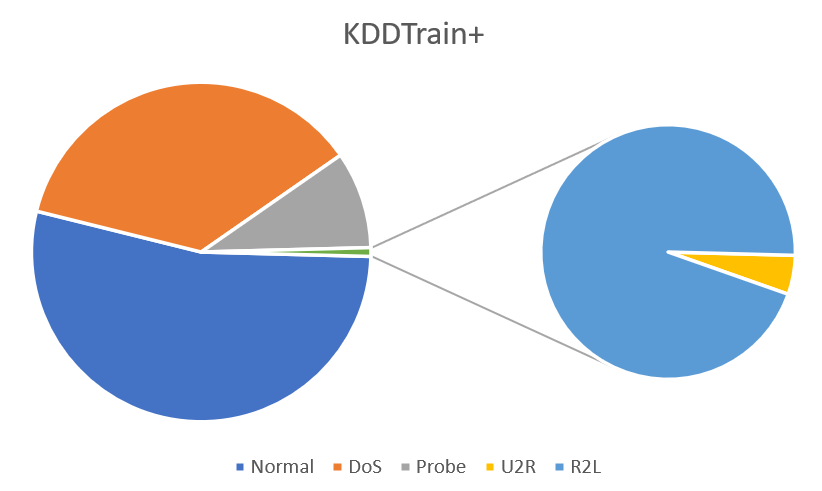
\includegraphics[width=0.4\textwidth]{kddtraindistribution.png}
	}
	\hspace{36pt}
	\subcaptionbox{测试集\label{fig:kddtestdistribution}}[0.4\textwidth]{
		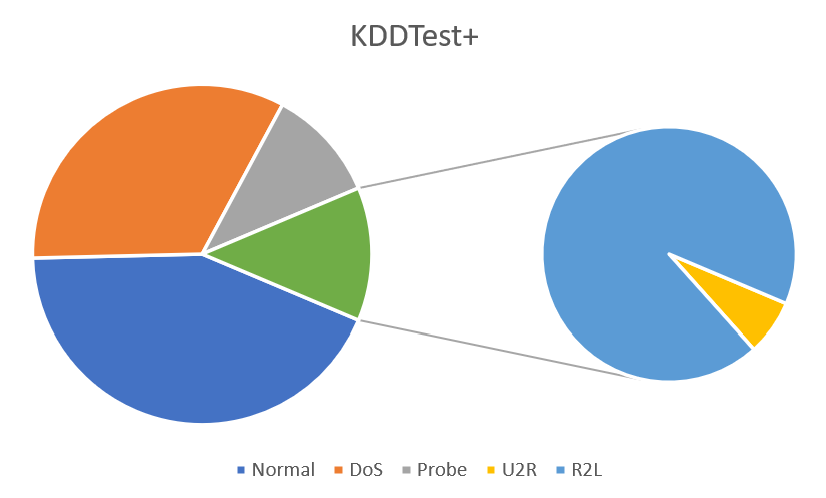
\includegraphics[width=0.4\textwidth]{kddtestdistribution.png}
	}
	\caption{NSL-KDD完整数据集分类占比饼状图}
\end{figure}

通过以上图表可知数据集中不同攻击类型的数据分布不均衡,特别是U2R和R2L攻击类型的样本数量远少于其他类型。
这种不平衡分布对于训练入侵检测系统模型来说是一个挑战,因为模型可能会在较多样本的攻击类型上表现更好,而在样本较少的攻击类型上表现不佳。
此外,从KDDTrain+到KDDTest+,攻击类型的分布变化表明,测试集可能代表了与训练集不同的攻击环境,这要求模型具备良好的泛化能力,以适应不同的攻击行为和模式。\par

\textbf{2.实验设计}\par
本文首先使用UNSW-NB15作为旧任务数据集,并将其划分为训练集和测试集。
具体而言,我们选取数据集中的80\%作为训练集,用于训练模型以获取基本的网络攻击检测能力;剩余的20\%则作为测试集,用于初步评估模型的性能。
随后,我们直接利用NSL-KDD提供的训练集文件中的数据作为新任务数据集,同时采用NSL-KDD提供的测试集文件中的数据作为我们的测试集。
为了进行增量学习,我们采用批量读取的方式处理新任务数据集。
每个增量学习阶段设定读取1,000个样本,同时设定记忆集的大小与每阶段训练集的大小保持一致,均为1,000。
在增量学习的每个批次中,我们都进行100轮的训练,以确保模型能够充分学习当前批次的数据。\par

\textbf{3.实验结果与分析}\par
为验证本文方案进行增量学习后的效果,我们选取了一系列模型,包括DT(决策树)、LR(逻辑回归)、KNN(K近邻)、NB(朴素贝叶斯)、Ada(AdaBoost增强)、ResN(残差神经网络)、BiG(双向门控循环单元)、RB-NMF(未经多模态特征融合的残差神经网络与双向门控循环单元)、RB-MF(经过多模态特征融合的残差神经网络与双向门控循环单元)、RB-MF with iCaRL(基于iCaRL的RB-MF模型),以及RB-MF with iCaRL and GA(结合了遗传算法记忆集抽样优化的RB-MF with iCaRL模型),并对这些模型进行了增量学习实验。
当所有新任务训练集的内容学习完成后,我们将新任务测试集与旧任务测试集进行合并形成混合测试集,用以评估各模型在混合数据集上的性能。\par

图~\ref{fig:acc_icarl}展示了各个模型在新任务测试集上的准确率表现。
\begin{figure}[h]
	\centering
	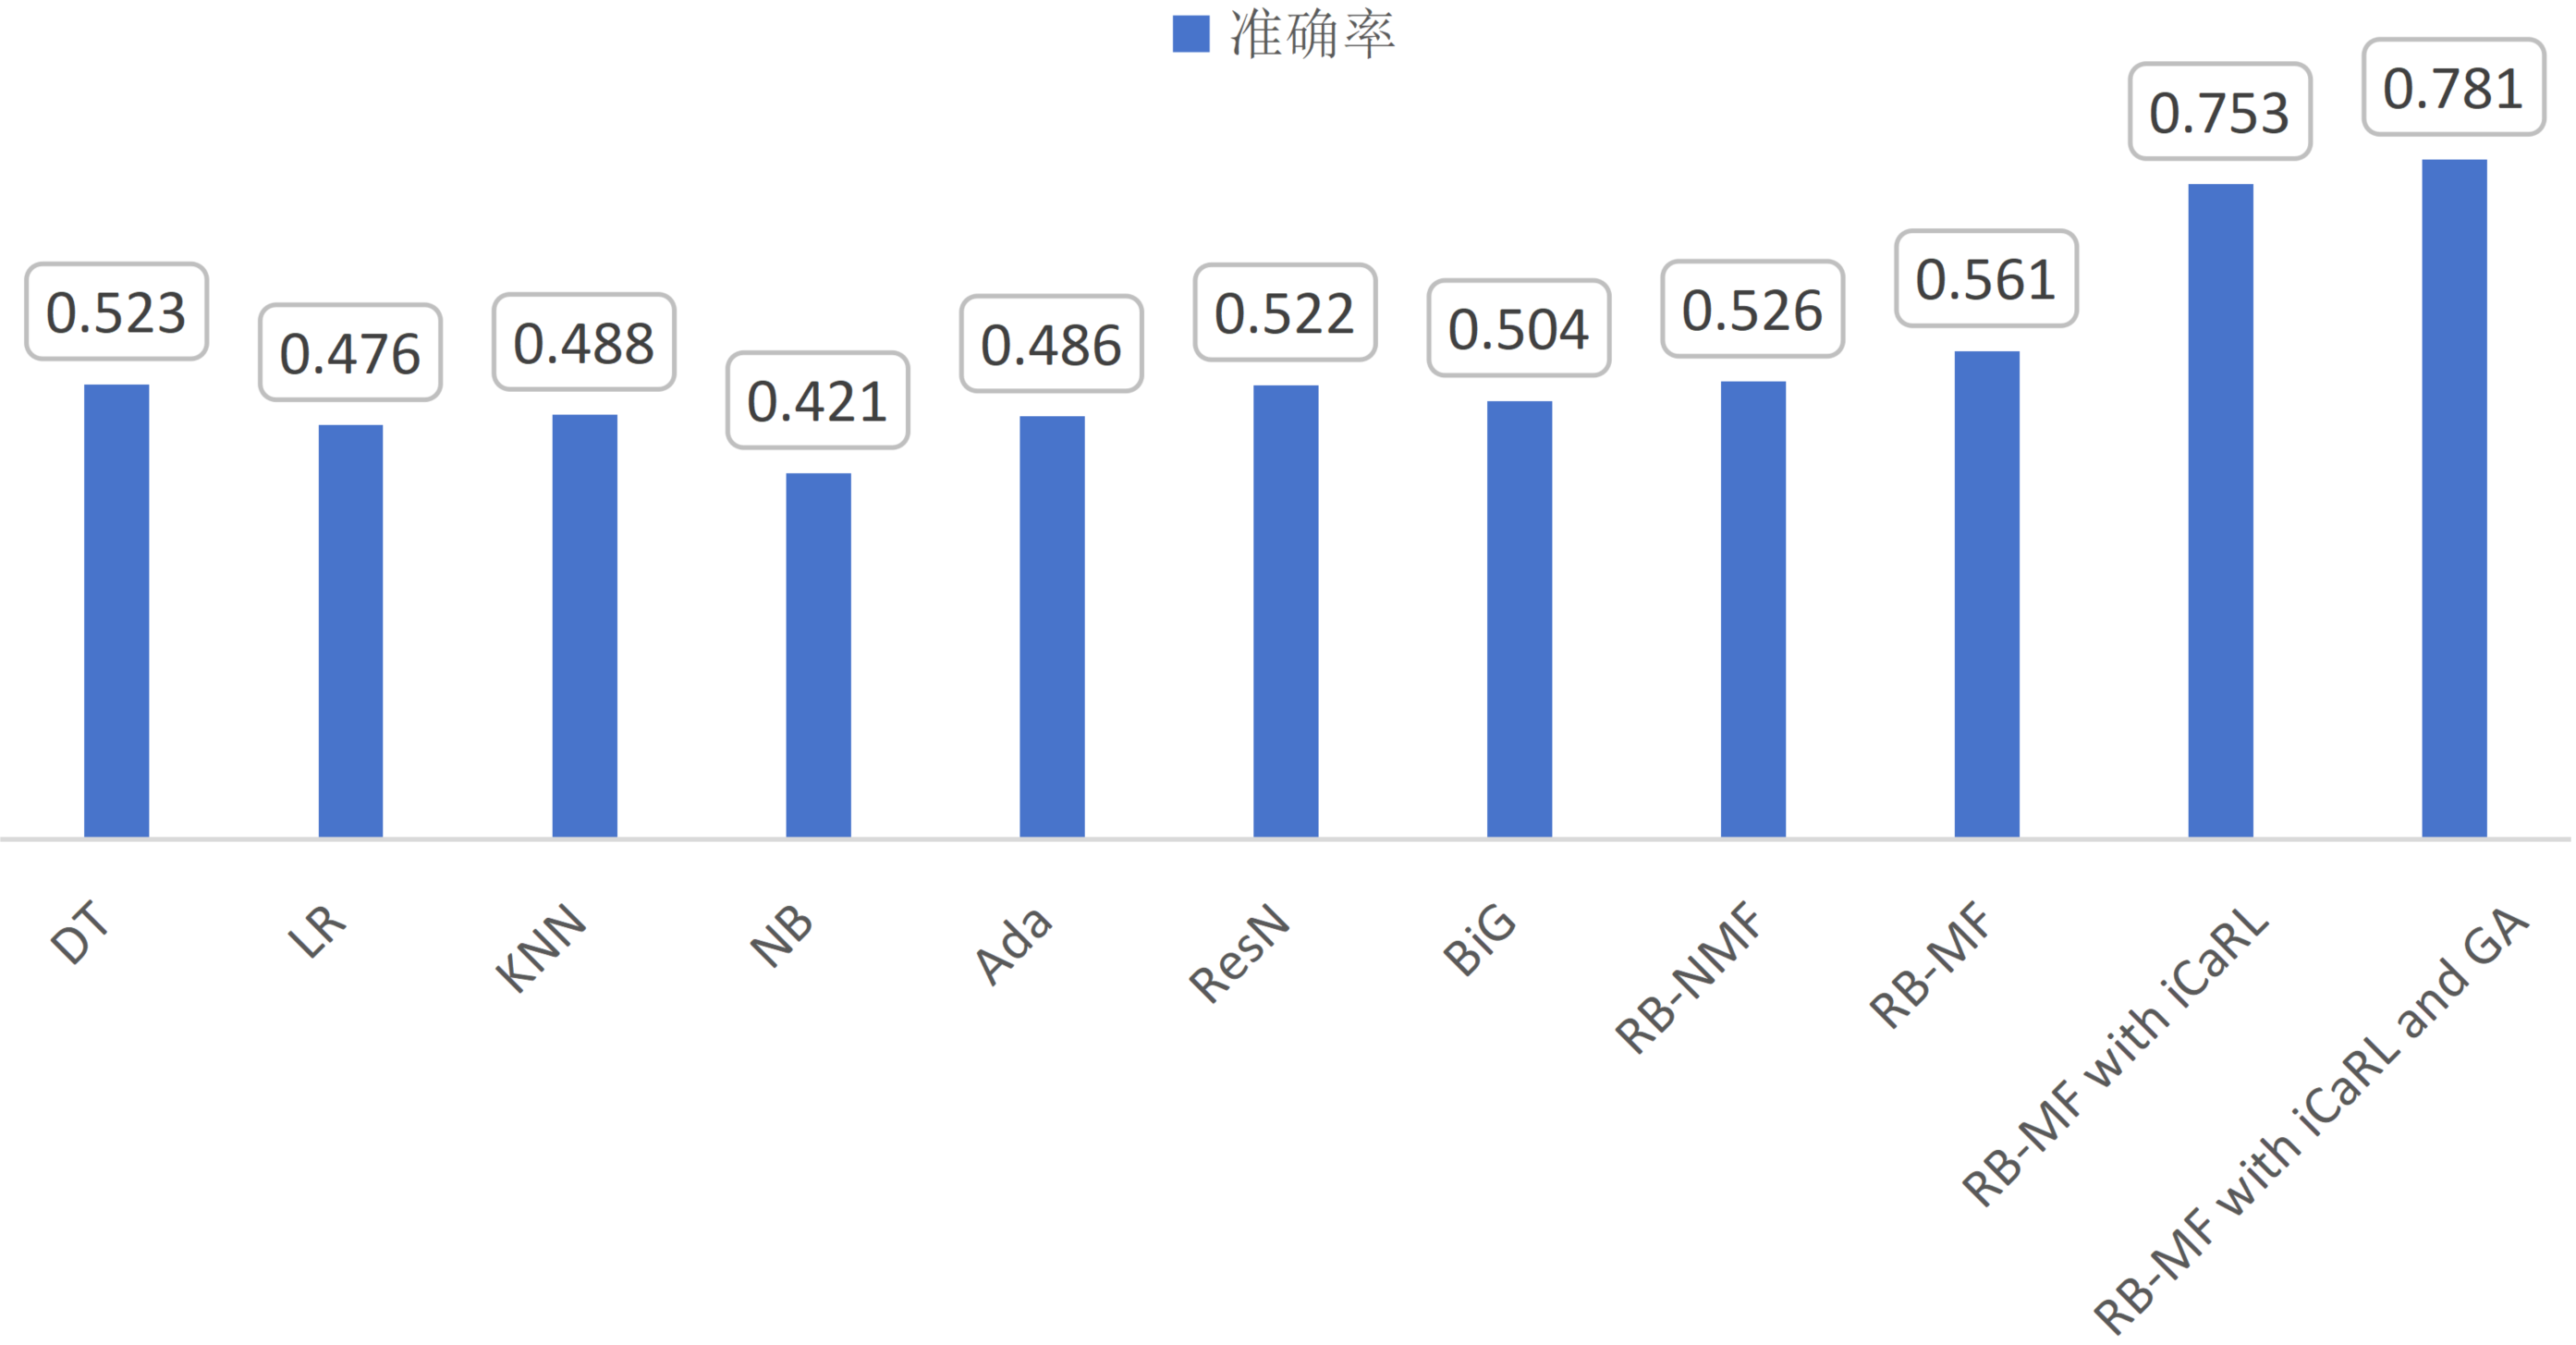
\includegraphics[width=0.8\textwidth]{icarl_accuracy.png}
	\caption{增量学习后各模型在混合测试集上准确率对比柱状图}
	\caption{增量学习后各模型在混合测试集上准确率对比柱状图}
	\label{fig:acc_icarl}
\end{figure}
从图中可以明显看出,引入iCaRL策略后,模型的准确率得到了显著提升。
这一结果充分证明了iCaRL策略在保持模型对旧知识记忆的同时学习新知识的有效性。
特别值得注意的是,本文提出的基于遗传算法的记忆集抽样优化方法在iCaRL的基础上进一步提高了RB-MF模型的准确率。
这表明该方法能够有效保留模型的记忆能力,提升其在增量学习过程中的性能。
然而,对于其他模型如DT、LR、KNN、NB和Ada,在进行增量学习后面对新任务数据集与旧任务数据集的混合测试集时表现并不理想。
这可能是因为这些模型在学习新知识的过程中,容易遗忘旧知识,导致在混合测试集上的性能下降。
下面的实验是对这一问题的具体验证。

图~\ref{fig:acc_forget}是每十个增量学习阶段后模型在旧任务数据集上的准确率变化。
\begin{figure}[h]
	\centering
	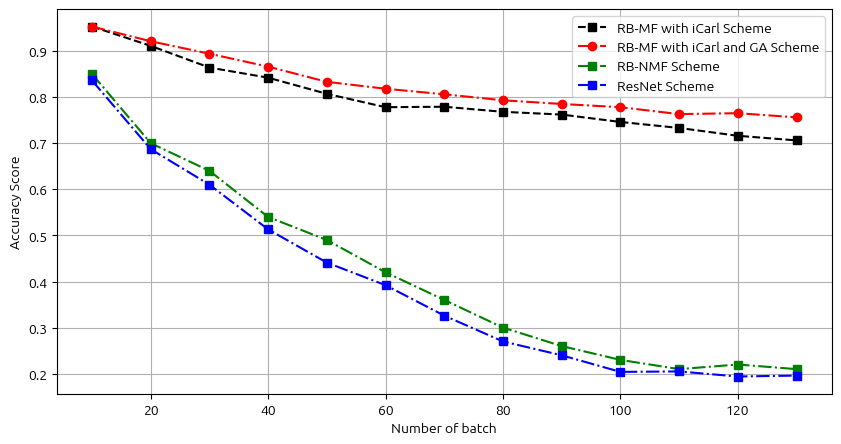
\includegraphics[width=0.8\textwidth]{forget.png}
	\caption{增量学习后模型在旧任务数据集上的准确率下降对比柱状图}
	\label{fig:acc_forget}
\end{figure}
\par
从图中可以看出,没有结合iCaRL策略的模型在经过增量学习后,其准确率迅速下降,
而结合了iCaRL策略的RB-MF模型则能够较好地保持准确率,最终模型的准确率保持在70\%以上。
这表明模型在没有采取额外策略的情况下学习新知识会导致对旧知识的遗忘。
特别值得一提的是,当使用本文所提出的基于遗传算法的记忆集抽样优化策略后,模型的准确率仍能得到进一步的提升。
这表明了本文提出的记忆集抽样优化策略能有效增强模型的增量学习效果。

\section{本章小结}
在本章中,我们提出了一种多模态特征融合模型,该模型基于残差网络与双向门控循环单元,旨在提升传统网络攻击检测技术的准确性。
通过在实验数据集上与多种经典机器学习和深度学习模型进行详尽的对比分析,我们的模型展现出了显著的性能优势。
为了进一步应对不断变化的网络攻击环境带来的挑战,我们引入了iCaRL技术,设计了一种基于多模态特征融合的增量学习方案。
这一方案旨在确保模型在维持对原有网络攻击的高效识别能力的同时,不断适应并学习新型的网络攻击模式。
通过持续的学习,我们的模型能够更好地应对不断变化的网络环境,提升整体的安全防护能力。
此外,我们针对增量学习过程中使用的记忆集,提出了一种基于遗传算法的抽样优化方法。
通过这一方法,我们能够更加高效地利用有限的资源,提升增量学习的效率和准确性。
在实验中,我们以UNSW-NB15与NSL-KDD分别作为新旧数据集,与多种经典机器学习和深度学习模型进行了对比分析。
实验结果表明,我们的增量学习方案能够显著增强模型的学习能力,实现了对旧知识的有效保留和新知识的快速学习。
%%================================================
%% Filename: chap04.tex
%% Encoding: UTF-8
%% Author: Yuan Xiaoshuai - yxshuai@gmail.com
%% Created: 2012-04-28 00:15
%% Last modified: 2019-11-06 17:39
%%================================================
\chapter{基于特征选择优化的ResNet-BiGRU 分类检测模型}
\label{cha:ResNet-BiGRU}

\section{插图示例}
\label{sec:figure}

\subsection{\LaTeX~中推荐使用的图片格式}

在~\LaTeX~中应用最多的图片格式是~EPS(Encapsulated PostScript)格式,它是一种
专用的打印机描述语言,常用于印刷或打印输出。EPS~格式图片可通过多种方式生成,
如果使用命令行界面,则可以用 ImageMagick,其可将其它格式图片转换为~EPS~格式图
片,同时还可以锐化图片,使图片的局部清晰一些。

ImageMagick 包含多个命令行程序,其中最常用的是 \texttt{convert}。
\begin{shell}
convert [可选参数] 原文件名.原扩展名 新文件名.eps
\end{shell}

除此之外,一些文字处理软件和科学计算软件也支持生成~EPS~格式的文件,可用“另存
为”功能查看某款软件是否能够将图片以~EPS~格式的形式保存。

\subsection{插入单幅图形}

插图通常需要占据大块空白,所以在文字处理软件中用户经常需要调整插图的位置。
\LaTeX~有一个 \texttt{figure} 环境可以自动完成这样的任务,这种自动调整位置的环
境称作浮动环境(float),之后还会介绍表格浮动环境。

单张图片插入形式如图~\ref{fig:golfer}~所示。
\begin{figure}[htbp]
\centering
\includegraphics[width = 0.3\textwidth]{golfer}
\caption{打高尔夫球的人}
\label{fig:golfer}
\end{figure}

\begin{latex}
\begin{figure}[htbp]
\centering
\includegraphics[width=0.3\textwidth]{golfer}
\caption{打高尔夫球的人}
\label{fig:golfer}%应放在\caption{}之后,否则引用时指向的是前一个插图
\end{figure}
\end{latex}

上述代码中,\verb|[htbp]| 选项用来指定插图排版的理想位置,这几个字母分别代表
~here、top、bottom、float page,也就是固定位置、页顶、页尾、单独的浮动页。可
以使用这几个字母的任意组合,一般不推荐单独使用 \verb|[h]|。如果要强制固定浮动
图形的位置,还可以用 \textbf{float} 宏包的 \verb|[H]| 选项。

\subsection{插入多幅图形}

\subsubsection*{并排摆放,共享标题}

当我们需要两幅图片并排摆放,并共享标题时,可以在 \texttt{figure} 环境中使用两个
\begin{latex}
\includegraphics{}
\end{latex}
命令,如图~\ref{fig:fanqingfuming}~所示。

\begin{latex}
\begin{figure}[htbp]
\centering
\includegraphics[width=0.3\textwidth]{qingming}
\hspace{36pt}
\includegraphics[width=0.3\textwidth]{fanfu}
\caption{反清复明}
\label{fig:fanqingmuming}
\end{figure}
\end{latex}

\begin{figure}[htbp]
\centering
\includegraphics[width=0.3\textwidth]{qingming}
\hspace{36pt}
\includegraphics[width=0.3\textwidth]{fanfu}
\caption{反清复明}
\label{fig:fanqingfuming}
\end{figure}

\subsubsection*{并排摆放,各有标题}

如果想要两幅并排的图片各有自己的标题,可以在 \texttt{figure} 环境中使用两个
 \texttt{minipage} 环境,每个环境里插入一个图,如图~\ref{fig:qingming}~和
~\ref{fig:fanfu}~所示。

\begin{latex}
\begin{figure}[htbp]
\centering
\begin{minipage}[t]{0.3\textwidth}
    \centering
    \includegraphics[width=\textwidth]{qingming}
    \caption{清明}
    \label{fig:qingming}
\end{minipage}
\hspace{36pt}
\begin{minipage}[t]{0.3\textwidth}
    \centering
    \includegraphics[width=\textwidth]{fanfu}
    \caption{反复}
    \label{fig:fanfu}
\end{minipage}
\end{figure}
\end{latex}

\begin{figure}[htbp]
\centering
\begin{minipage}[t]{0.3\textwidth}
    \centering
    \includegraphics[width=\textwidth]{qingming}
    \caption{清明}
    \label{fig:qingming}
\end{minipage}
\hspace{36pt}
\begin{minipage}[t]{0.3\textwidth}
    \centering
    \includegraphics[width=\textwidth]{fanfu}
    \caption{反复}
    \label{fig:fanfu}
\end{minipage}
\end{figure}

\subsubsection*{并排摆放,共享标题,各有子标题}

如果想要两幅并排的图片共享一个标题,并各有自己的子标题,可以使用
\textbf{subcaption} 宏包提供的
\begin{latex}
\subcaptionbox{<title>}[<width>]{<insertfigure>}
\end{latex}
命令,如图~\ref{fig:subfig_a}~和~\ref{fig:subfig_b}~所示。

\begin{latex}
\begin{figure}[htbp]
  \centering
  \subcaptionbox{清明\label{fig:subfig_a}}[0.3\textwidth]{
      \includegraphics[width=0.3\textwidth]{qingming}
  }
  \hspace{36pt}
  \subcaptionbox{反复\label{fig:subfig_b}}[0.3\textwidth]{
      \includegraphics[width=0.3\textwidth]{fanfu}
  }
  \caption{反清复明}
\end{figure}
\end{latex}

每个子图可以有各自的引用,就象这个样子:\ref{fig:subfig_a}、
\ref{fig:subfig_b}。

\begin{figure}[htbp]
\centering
\subcaptionbox{清明\label{fig:subfig_a}}[0.3\textwidth]{
    \includegraphics[width=0.3\textwidth]{qingming}
}
\hspace{36pt}
\subcaptionbox{反复\label{fig:subfig_b}}[0.3\textwidth]{
    \includegraphics[width=0.3\textwidth]{fanfu}
}
\caption{反清复明}
\end{figure}

\section{表格示例}
\label{sec:table}

模板中关于表格的宏包有四个:\textbf{tabularx}、\textbf{multirow}、
\textbf{longtable} 和\textbf{booktabs}。长表格还可以用\textbf{supertabular},
可以方便地在表格下方加入脚注。

\subsection{普通表格的绘制方法}

\texttt{table} 环境是一个将表格嵌入文本的浮动环境,其标题和交叉引用的用法类似
于上一节提到的图形浮动环境 \texttt{figure}。该环境提供了最简单的表格功能,常用命令如下
\begin{latex}
\hline % 横线
|      % 竖线
&      % 分列
\\     % 换行
l c r  % 横向居中、居左、居右对齐  
\end{latex}

科技文献中常使用三线表格,因此需要调用 \textbf{booktabs} 宏包,三条横线就分别
用
\begin{latex}
\toprule
\midrule
\bottomrule
\end{latex}
等命令表示。其标准格式如表~\ref{table1}~所示。

\begin{table}[htbp]
\caption{文献类型和标识代码}
\label{table1}
\centering
\begin{tabular}{cccc}
\toprule
文献类型 & 标识代码 & 文献类型 & 标识代码\\
\midrule
普通图书 & M &  会议录 & C\\
汇编 & G & 报纸 & N\\
期刊 & J & 学位论文 & D\\
报告 & R & 标准 & S\\
专利 & P & 数据库 & DB\\
计算机程序 & CP & 电子公告 & EB\\
\bottomrule
\end{tabular}
\end{table}

绘制该表格的代码如下:
\begin{latex}
\begin{table}[htbp]
\caption{表格标题}
\label{标签名}
\centering
\begin{tabular}{cc...c}
\toprule
表头第1个格   & 表头第2个格   & ... & 表头第n个格  \\
\midrule
表中数据(1,1) & 表中数据(1,2) & ... & 表中数据(1,n)\\
表中数据(2,1) & 表中数据(2,2) & ... & 表中数据(2,n)\\
...................................................\\
表中数据(m,1) & 表中数据(m,2) & ... & 表中数据(m,n)\\
\bottomrule
\end{tabular}
\end{table}
\end{latex}

\subsection{长表格的绘制方法}

长表格是当表格在当前页排不下而需要转页接排的情况下所采用的一种表格环境。若长
表格仍按照普通表格的绘制方法来获得,其所使用的 \verb|table| 浮动环境无法实现
表格的换页接排功能,表格下方过长部分会排在表格第1页的页脚以下。

\begin{longtable}{l@{\hspace{6.5mm}}l@{\hspace{5.5mm}}l}
\multicolumn{3}{c}{续表~\thetable\hskip1em 中国省级行政单位一览}\\
\toprule 名称 & 简称 & 省会或首府  \\ \midrule
\endhead
\caption{中国省级行政单位一览}
\label{table2}\\
\toprule 名称 & 简称 & 省会或首府  \\ \midrule
\endfirsthead
\bottomrule
\multicolumn{3}{r}{续下页}\\
\endfoot
\bottomrule
\endlastfoot
北京市 & 京 & 北京\\
天津市 & 津 & 天津\\
河北省 & 冀 & 石家庄市\\
山西省 & 晋 & 太原市\\
内蒙古自治区 & 蒙 & 呼和浩特市\\
辽宁省 & 辽 & 沈阳市\\
吉林省 & 吉 & 长春市\\
黑龙江省 & 黑 & 哈尔滨市\\
上海市 & 沪/申 & 上海\\
江苏省 & 苏 & 南京市\\
浙江省 & 浙 & 杭州市\\
安徽省 & 皖 & 合肥市\\
福建省 & 闽 & 福州市\\
江西省 & 赣 & 南昌市\\
山东省 & 鲁 & 济南市\\
河南省 & 豫 & 郑州市\\
湖北省 & 鄂 & 武汉市\\
湖南省 & 湘 & 长沙市\\
广东省 & 粤 & 广州市\\
广西壮族自治区 & 桂 & 南宁市\\
海南省 & 琼 & 海口市\\
重庆市 & 渝 & 重庆\\
四川省 & 川/蜀 & 成都市\\
贵州省 & 黔/贵 & 贵阳市\\
云南省 & 云/滇 & 昆明市\\
西藏自治区 & 藏 & 拉萨市\\
陕西省 & 陕/秦 & 西安市\\
甘肃省 & 甘/陇 & 兰州市\\
青海省 & 青 & 西宁市\\
宁夏回族自治区 & 宁 & 银川市\\
新疆维吾尔自治区 & 新 & 乌鲁木齐市\\
香港特别行政区 & 港 & 香港\\
澳门特别行政区 & 澳 & 澳门\\
台湾省 & 台 & 台北市\\
北京市 & 京 & 北京\\
天津市 & 津 & 天津\\
河北省 & 冀 & 石家庄市\\
山西省 & 晋 & 太原市\\
内蒙古自治区 & 蒙 & 呼和浩特市\\
辽宁省 & 辽 & 沈阳市\\
吉林省 & 吉 & 长春市\\
黑龙江省 & 黑 & 哈尔滨市\\
上海市 & 沪/申 & 上海\\
江苏省 & 苏 & 南京市\\
浙江省 & 浙 & 杭州市\\
安徽省 & 皖 & 合肥市\\
福建省 & 闽 & 福州市\\
江西省 & 赣 & 南昌市\\
山东省 & 鲁 & 济南市\\
河南省 & 豫 & 郑州市\\
湖北省 & 鄂 & 武汉市\\
湖南省 & 湘 & 长沙市\\
广东省 & 粤 & 广州市\\
广西壮族自治区 & 桂 & 南宁市\\
海南省 & 琼 & 海口市\\
重庆市 & 渝 & 重庆\\
四川省 & 川/蜀 & 成都市\\
贵州省 & 黔/贵 & 贵阳市\\
云南省 & 云/滇 & 昆明市\\
西藏自治区 & 藏 & 拉萨市\\
陕西省 & 陕/秦 & 西安市\\
甘肃省 & 甘/陇 & 兰州市\\
青海省 & 青 & 西宁市\\
宁夏回族自治区 & 宁 & 银川市\\
新疆维吾尔自治区 & 新 & 乌鲁木齐市\\
香港特别行政区 & 港 & 香港\\
澳门特别行政区 & 澳 & 澳门\\
台湾省 & 台 & 台北市\\
\end{longtable}

表格~\ref{table2}~第~2~页的标题和表头是通过代码自动添加上去的。若表格在页面中
的竖直位置发生了变化,其在第~2~页及之后各页的标题和表头位置能够始终处于各页的
最顶部,无需调整。

\subsection{列宽可调表格的绘制方法}

论文中能用到列宽可调表格的情况共有两种,一种是当插入的表格某一单元格内容过长
以至于一行放不下的情况,另一种是当对公式中首次出现的物理量符号进行注释的情况
,这两种情况都需要调用 \textbf{tabularx} 宏包。下面将分别对这两种情况下可调表格的绘制
方法进行阐述。

\subsubsection{表格内某单元格内容过长的情况}

首先给出这种情况下的一个例子如表~\ref{table3}~所示。

\begin{table}[htbp]
\caption{最小的三个正整数的英文表示法}
\label{table3}
\begin{tabularx}{\textwidth}{llX}
\toprule
Value & Name & Alternate names, and names for sets of the given size\\
\midrule
1 & One & ace, single, singleton, unary, unit, unity\\
2 & Two & binary, brace, couple, couplet, distich, deuce, double, doubleton, duad, duality, duet, duo, dyad, pair, snake eyes, span, twain, twosome, yoke\\
3 & Three & deuce-ace, leash, set, tercet, ternary, ternion, terzetto, threesome, tierce, trey, triad, trine, trinity, trio, triplet, troika, hat-trick\\\bottomrule
\end{tabularx}
\end{table}

绘制该表格的代码如下:

\begin{latex}
\begin{table}[htbp]
\caption{表格标题}
\label{标签名}
\begin{tabularx}{\textwidth}{l...X...l}
\toprule
表头第1个格   & ... & 表头第X个格   & ... & 表头第n个格  \\
\midrule
表中数据(1,1) & ... & 表中数据(1,X) & ... & 表中数据(1,n)\\
表中数据(2,1) & ... & 表中数据(2,X) & ... & 表中数据(2,n)\\
.........................................................\\
表中数据(m,1) & ... & 表中数据(m,X) & ... & 表中数据(m,n)\\
\bottomrule
\end{tabularx}
\end{table}
\end{latex}

\texttt{tabularx} 环境共有两个必选参数:第1个参数用来确定表格的总宽度,这里取
为排版表格能达到的最大宽度——正文宽度 \verb|\textwidth|;第2个参数用来确定每列
格式,其中标为 \verb|X| 的项表示该列的宽度可调,其宽度值由表格总宽度确定。标
为 \verb|X| 的列一般选为单元格内容过长而无法置于一行的列,这样使得该列内容能
够根据表格总宽度自动分行。若列格式中存在不止一个 \verb|X| 项,则这些标为
\verb|X| 的列的列宽相同,因此,一般不将内容较短的列设为 \verb|X| 。标为
\verb|X| 的列均为左对齐,因此其余列一般选为 \verb|l| (左对齐),这样可使得表格
美观,但也可以选为 \verb|c| 或 \verb|r|。

\subsubsection{对物理量符号进行注释的情况}

为使得对公式中物理量符号注释的转行与破折号“——”后第一个字对齐,此处最
好采用表格环境。此表格无任何线条,左对齐,且在破折号处对齐,一共有“式中”二字
、物理量符号和注释三列,表格的总宽度可选为文本宽度,因此应该采用
\texttt{tabularx} 环境。由该环境生成的对公式中物理量符号进行注释的公式如式
(\ref{eq:1})所示。

\begin{equation}
\label{eq:1}
\ddot{\symbf{\rho}}-\frac{\mu}{R_t^3}\left(3\symbf{R_t}\frac{\symbf{R_t\rho}}{R_t^2}-\symbf{\rho}\right)=\symbf{a}
\end{equation}
\begin{flushleft}
\renewcommand\arraystretch{1.25}
\begin{tabularx}{\textwidth}{@{}>{\normalsize\rm}l@{\quad}>{\normalsize\rm}l@{——}>{\normalsize\rm}X@{}}
式中& $\symbf{\rho}$ &追踪飞行器与目标飞行器之间的相对位置矢量;\\
&  $\ddot{\symbf{\rho}}$&追踪飞行器与目标飞行器之间的相对加速度;\\
&  $\symbf{a}$   &推力所产生的加速度;\\
&  $\symbf{R_t}$ & 目标飞行器在惯性坐标系中的位置矢量;\\
&  $\omega_{t}$ & 目标飞行器的轨道角速度;\\
&  $\symbf{g}$ & 重力加速度,$=\frac{\mu}{R_{t}^{3}}\left(
3\symbf{R_{t}}\frac{\symbf{R_{t}\rho}}{R_{t}^{2}}-\symbf{\rho}\right)=\omega_{t}^{2}\frac{R_{t}}{p}\left(
3\symbf{R_{t}}\frac{\symbf{R_{t}\rho}}{R_{t}^{2}}-\symbf{\rho}\right)$,这里~$p$~是目标飞行器的轨道半通径。
\end{tabularx}\vspace{.5ex}%TODO : 注释内容自动转页接排
\end{flushleft}

其中生成注释部分的代码及其说明如下:
\begin{latex}
\begin{tabularx}{\textwidth}{@{}l@{\quad}l@{——}X@{}}
式中 & symbol-1 & symbol-1的注释内容;\\
     & symbol-2 & symbol-2的注释内容;\\
     .............................;\\
     & symbol-m & symbol-m的注释内容。
\end{tabularx}
\end{latex}

\texttt{tabularx} 环境的第1个参数为正文宽度,第2个参数里面各个符号的意义为:
\begin{itemize}
\item 第1个@{}表示在“式中”二字左侧不插入任何文本,“式中”二字能够在正文中左对
齐,若无此项,则“式中”二字左侧会留出一定的空白;
\item \verb|@{\quad}| 表示在“式中”和物理量符号间插入一个空铅宽度的空白;
\item \verb|@{——}| 实现插入破折号的功能;
\item 第2个 \verb|@{}| 表示在注释内容靠近正文右边界的地方能够实现右对齐。
\end{itemize}

\subsection{小页中的脚注}

关于小页中的脚注,请看下面的例子:
 
\begin{minipage}[t]{\linewidth-\parindent}
柳宗元,字子厚(773-819),河东(今永济县)人\footnote{山西永济水饺。},是唐
代杰出的文学家,哲学家,同时也是一位政治改革家。与韩愈共同倡导唐代古文运动,
并称韩柳\footnote{唐宋八大家之首二位。}。
\end{minipage}

\section{数学公式示例}
\label{sec:equation}

\LaTeX{} 的数学公式有两种形式:行间(inline)模式和独立(display)模式。前者是
指在正文中插入数学内容;后者独立排列,可以有或者没有编号。行间公式和无编号独立
公式都有多种输入方法,一般行间公式用 \verb|$|\ldots \verb|$|,无编号独立公式用
\verb|\[|\ldots \verb|\]|。有编号独立公式则需要用 \texttt{equation} 环境。

注意一下公式显示模式的不同,这个公式为行间模式:
$\lim_{n \to \infty} \sum_{k=1}^n \frac{1}{k^2} = \frac{\pi^2}{6}$;下面的公式
是独立模式:
\[\lim_{n \to \infty} \sum_{k=1}^n \frac{1}{k^2} = \frac{\pi^2}{6}\]

\subsection{多行公式}

\textbf{amsmath} 宏包提供了额外的行间独立(display)公式的结构,主要用于一个
公式太长一行放不下,或几个公式需要写成一组的情况,该宏包主要提供以下几个环境
:
\begin{center}
\begin{tabular}[c]{cccc}
equation & align & gather & split \\
flalign & multline & alignat &  \\
\end{tabular}
\end{center}

除了 \texttt{split} 外,其余环境均提供带*的版本,不生成公式编号。

\subsubsection{长公式}

对于多行不需要对齐的长公式,我们可以用 \texttt{multline} 环境。
\begin{multline}
\framebox[.65\columnwidth]{A}\\
\framebox[.5\columnwidth]{B}\\
\shoveright{\framebox[.5\columnwidth]{C}}\\
\framebox[.65\columnwidth]{D}
\end{multline}

其代码如下:
\begin{latex}
\begin{multline}
\framebox[.65\columnwidth]{A}\\
\framebox[.5\columnwidth]{B}\\
\shoveright{\framebox[.tt\columnwidth]{C}}\\
\framebox[.65\columnwidth]{D}
\end{multline}
\end{latex}

\texttt{multline} 环境用于单行放不下的长公式,其第一行及最后一行分别居左、居右
对齐,两端均缩进距离 \verb|\multlinegap|;其它行则默认居中排布,但可以用个命令
\verb|\shoveleft|、\verb|\shoveright| 分别使居左或居右排布。

需要对齐的长公式可以用 \texttt{split} 环境,它本身不能单独使用,因此也称作次环境
,必须包含在 \texttt{equation} 或其它数学环境内。\texttt{split} 环境用 \verb|\\| 
和 \verb|&| 来分行和设置对齐位置。
\begin{equation}
\begin{split}
H_c&=\frac{1}{2n} \sum^n_{l=0}(-1)^{l}(n-{l})^{p-2}
\sum_{l _1+\dots+ l _p=l}\prod^p_{i=1} \binom{n_i}{l _i}\\
&\quad\cdot[(n-l)-(n_i-l_i)]^{n_i-l_i}\cdot
\Bigl[(n-l)^2-\sum^p_{j=1}(n_i-l_i)^2\Bigr].
\end{split}
\label{eqn:barwq}
\end{equation}

\subsubsection{公式组}

不需要对齐的公式组用 \texttt{gather} 环境,该环境中的公式均居中排布,各公式间用
\verb|\\| 分开;需要对齐的用 \texttt{align},在该环境中使用 \verb|\text| 命令可
以生成对单独公式的注释。
\begin{gather}
  first equation\\
  \begin{split}
    second & equation\\
           & on twolines
  \end{split}
\end{gather}

\begin{align}
 x & = y_1-y_2+y_3-y_5+y_8-\dots && \text{by \eqref{eqn:barwq}}\\
   & = y'\circ y^*               && \text{by \eqref{eqn:barwq}}\\
   & = y(0) y'                   && \text{by Axiom 1.}
\end{align}

就像单独的行间公式一样,使用 \texttt{gather}、\texttt{align} 和
\texttt{alignat} 环境生成的公式组中的每个公式也都是占据整个文本的宽度,因此
这样的公式组两侧不能再添加其它内容,比如大括号等。不过相应地用
\texttt{gathered}、\texttt{aligned} 和 \texttt{alignedat} 环境则生成仅占据
实际公式宽度的公式组。
\begin{equation*}
\left. \begin{aligned}
  \symbf{B'}&=-\symbfit{\partial}\times \symbf{E},\\
  \symbf{E'}&=\symbfit{\partial}\times \symbf{B} - 4\pi j,
\end{aligned}
\right\}
\qquad \text{Maxwell's equations}
\end{equation*}

有多种条件的公式组用 \texttt{cases} 次环境。
\[ P_{r-j}=\begin{cases}
  0& \text{if $r-j$ is odd},\\
  r!\,(-1)^{(r-j)/2}& \text{if $r-j$ is even}.
\end{cases} \]

这里仅简单介绍了 \textbf{amsmath} 的功能,更详尽的说明可参见该宏包的文档。

\subsection{定理和证明}

\zzuthesis{} 定义了常用的数学环境:
\begin{center}
\begin{tabular}{*{7}{l}}\hline
  theorem & definition & lemma & corollary &\\
  定理 & 定义 & 引理 & 推论 &\\\hline
\end{tabular}
\end{center}

以上环境的定义采用 \textbf{amsthm} 宏包提供的 \verb|\newtheorem| 命令,其语法
如下:

\begin{latex}
\newtheorem{环境名}[编号延续]{显示名}[编号层次]
\end{latex}

下面是应用示例:
\begin{definition}
Java是一种跨平台的编程语言。
\end{definition}

\begin{theorem}
咖啡因会使人的大脑兴奋。
\end{theorem}

\begin{lemma}
茶和咖啡都会使人兴奋。
\end{lemma}

\begin{corollary}
晚上喝咖啡会导致失眠。
\end{corollary}

\texttt{proof} 环境可以用来输入证明,它会在结尾输入一个 QED 符号
\footnote{拉丁语~quod erat demonstrandum~的缩写。}。

\begin{proof}[命题“物质无限可分”的证明]
一尺之棰,日取其半,万世不竭。
\end{proof}

% 参考文献、致谢、附录等
\backmatter

% \bibliographystyle{gbt7714-unsrt.bst}%符合国标 GB/T 7714-2015 的文献风格
\bibliographystyle{zzubib.bst}%学校规范中示例文献风格
\bibliography{ref/refs}%参考文献

% 附录
% 研究生论文:综述
% \makeatletter
% \ifzzu@bachelor\else
%   \include{data/review}
% \fi
% \makeatother

\makeatletter%致谢,研究生论文中在参考文献后,附录前
\ifzzu@bachelor\else
  %%================================================
%% Filename: ack.tex
%% Encoding: UTF-8
%% Author: Yuan Xiaoshuai - yxshuai@gmail.com
%% Created: 2012-01-12 18:09
%% Last modified: 2016-08-28 21:05
%%================================================
\begin{ack}

% 韶华易逝,光阴荏苒,余自入渝倏忽而又三年矣。曩者,离鲁地,弃吴越奔巴蜀,恢恢乎
% 若漏网之鲫,惶惶乎似惊弓之鸟,几无容身之地。幸遇刘徐二相荐,得拜于恩师魏公门下
% ,而今已历六秋。先生治学严谨,博通中外,蔚为家,研习学术,废寝忘食,已臻忘我之
% 境界。犹忆当年,乍入门墙,耻无寸功先生不以余愚钝,委以重托,是以矢勤矢勇,思惟
% 速战,毋负所托。然欲速不心忧如焚。全赖先生数次点拨,每自躬亲,甚于子夜,共为进
% 退,方有所成。于缀词成文,苦心孤诣,字斟句酌,独具匠心,深为叹服,并于耳提面命
% 之际益良多。先生之德才,若高山仰止,亦非庸庸如吾辈者所能望其项背。每至周常言:
% “修身者智之府也,爱施者仁之端也,取予者义之符也,耻辱者勇之决也立名者行之极也
% 。凡此五者,皆安身立命之本,不可偏废。”言之谆谆,听之诚若醍醐灌顶。退而思之,
% 果斯然也,大为拜服。兼之师母,待余恩厚,视若螟多得给养,感激涕零。余素朴陋,尚
% 无剖符丹书之功,反受此殊遇,非结草衔不可报也!今虽即辞师门,必常怀乌鸟之情,反
% 哺之心,诚不失其望也!

% 师门同侪,学强张骞,皆忠义之士,情同手足;乐至四国,许都耀琼,此良实,多蒙所助
% ;兰莉二姊,性行淑均,爱如姐弟。其他诸君,皆为志虑忠纯士,多有广益。区区不才,
% 有何德能,安得广助若此?感荷之心,亦自拳拳。实验中曾多次求教于杨(明莉)、杜(
% 军)二老师,受益匪浅;中心实验室(光辉)、鲜(晓红)二位老师及刘姊渝萍为实验工
% 作大开方便之门,谨表谢忱家中上至期颐之祖母,中至慈爱之父母、姊姊,下至始龀之甥
% 男,均不遗力以支持,融融亲情,曷其幸甚!谨撰此文,鱼传尺素,答报椿萱!

% 嗟乎!聚散无常,盛况难再;书不尽意,略陈固陋。临别赠言,幸承恩于公;登高作赋,
% 是所望于群贤。斗胆献拙,情之不已;一言均赋,四韵俱成。洒陵江,以酹逝去之岁月。

% \begin{center}
% 西入渝州已六霜,貔貅帐里铸鱼肠。\\
% 书山文海研学术,翠袖红巾戏皮黄。\\
% 莫叹时舛惟虎踞,且图运转季鹰扬。\\
% 今朝叩别师尊去,一片丹心化碧江。
% \footnote{重庆大学化工博士季孟波学位论文《抗溺水性气体多孔电极的研究》致谢词}
% \end{center}
时光荏苒,三年的硕士生涯即将画上句号。站在这个人生的十字路口,我回首望去,心中涌动着无尽的感慨与感激。在这段充满挑战与成长的旅程中,我得到了许多人的关心、帮助和支持,此刻,我想向他们表达我最深切的谢意。

首先,我要衷心感谢我的导师。您的严谨治学、勤奋工作的精神深深感染了我,为我树立了榜样。在您的悉心指导下,我不仅学会了如何进行学术研究,更学会了如何面对困难和挑战,不断超越自我。您的每一次指点都让我受益匪浅,您的每一次鼓励都让我信心倍增。您的教诲和关怀让我在学术道路上不断成长,您的支持和鼓励让我在人生道路上更加坚定。

其次,我要感谢实验室的同学们。我们一同度过了无数个日夜,共同经历了学术的磨砺和生活的点滴。我们互相支持、互相鼓励,一起探讨学术问题,一起分享生活感悟。你们的陪伴让我的研究生生涯充满了欢笑和温暖,你们的友谊是我人生中最宝贵的财富。

此外,我还要感谢我的家人。在我求学的道路上,你们始终是我最坚实的后盾。你们的爱如春风化雨,滋润着我的心田;你们的支持如灯塔指引,照亮我前行的道路。无论我走到哪里,你们都是我最强大的精神支柱。你们的理解和包容让我能够勇往直前,追求自己的梦想。

同时,我要感谢母校为我提供了如此优秀的学术环境和资源。在这里,我得以接触到前沿的学术思想,结识了许多优秀的师生。母校的培养和熏陶让我不仅在学术上取得了进步,更在人格上得到了提升。

最后,我要感谢所有在我求学路上给予过帮助和支持的人。你们的关心和帮助让我在困境中看到了希望,在挫折中找到了力量。你们的支持和鼓励是我不断前进的动力源泉。

即将离开校园,踏上新的人生征程,我会将这段宝贵的经历铭记在心,继续努力学习,不断提升自己。我会将所学所悟应用于实践,为社会的发展贡献自己的力量。我相信,在未来的日子里,我会以更加成熟、更加自信的姿态迎接挑战,创造属于自己的辉煌。

再次感谢所有帮助过我的人,愿我们未来的道路都充满阳光和希望,愿我们的友谊天长地久,愿我们的人生更加精彩纷呈!

\end{ack}

\fi
\makeatother

% 附录
% 本科生论文三个附录,分别是附表,外文翻译和外文原文
% 研究生论文无具体要求
\makeatletter
\ifzzu@bachelor
  \begin{appendix}
    \input{data/app01}
    \input{data/app02}
    \input{data/app03}
  \end{appendix}
\fi
\makeatother

\makeatletter%个人简历
\ifzzu@bachelor\else
  %%================================================
%% Filename: resume.tex
%% Encoding: UTF-8
%% Author: Yuan Xiaoshuai - yxshuai@gmail.com
%% Created: 2012-01-12 18:07
%% Last modified: 2016-08-28 21:09
%%================================================
\begin{resume}

  \resumeitem{个人简历}

  杨洪伟,男,山东临沂人
  
  2021.09-至今~郑州大学~网络空间安全~硕士学位
  
  2019.09-2021.06~山东航空学院~计算机科学与技术~学士学位

  \resumeitem{发表的学术论文} % 发表的和录用的合在一起

  \begin{enumerate}[{[}1{]}]
    \item Hongwei Yang,Gang Chen,Chunqian Guo.IGPPM: Interface Grouped Probabilistic Packet Marking Scheme for IP Traceback.2023 2nd International Conference on Informatics,Networking and Computing (ICINC 2023).
  % \item Yang Y, Ren T L, Zhang L T, et al. Miniature microphone with silicon-
  %   based ferroelectric thin films. Integrated Ferroelectrics, 2003,
  %   52:229-235. (SCI 收录, 检索号:758FZ.)
  % \item 杨轶, 张宁欣, 任天令, 等. 硅基铁电微声学器件中薄膜残余应力的研究. 中国机
  %   械工程, 2005, 16(14):1289-1291. (EI 收录, 检索号:0534931 2907.)
  % \item 杨轶, 张宁欣, 任天令, 等. 集成铁电器件中的关键工艺研究. 仪器仪表学报,
  %   2003, 24(S4):192-193. (EI 源刊.)
  % \item Yang Y, Ren T L, Zhu Y P, et al. PMUTs for handwriting recognition. In
  %   press. (已被 Integrated Ferroelectrics 录用. SCI 源刊.)
  % \item Wu X M, Yang Y, Cai J, et al. Measurements of ferroelectric MEMS
  %   microphones. Integrated Ferroelectrics, 2005, 69:417-429. (SCI 收录, 检索号
  %   :896KM.)
  % \item 贾泽, 杨轶, 陈兢, 等. 用于压电和电容微麦克风的体硅腐蚀相关研究. 压电与声
  %   光, 2006, 28(1):117-119. (EI 收录, 检索号:06129773469.)
  % \item 伍晓明, 杨轶, 张宁欣, 等. 基于MEMS技术的集成铁电硅微麦克风. 中国集成电路, 
  %   2003, 53:59-61.
  \end{enumerate}

  % \resumeitem{研究成果} % 有就写,没有就删除
  % \begin{enumerate}[{[}1{]}]
  % \item 任天令, 杨轶, 朱一平, 等. 硅基铁电微声学传感器畴极化区域控制和电极连接的
  %   方法: 中国, CN1602118A. (中国专利公开号.)
  % \item Ren T L, Yang Y, Zhu Y P, et al. Piezoelectric micro acoustic sensor
  %   based on ferroelectric materials: USA, No.11/215, 102. (美国发明专利申请号.)
  % \end{enumerate}
\end{resume}
%本科论文无要求
\fi
\makeatother

\makeatletter%致谢,本科论文在最后
\ifzzu@bachelor
  %%================================================
%% Filename: ack.tex
%% Encoding: UTF-8
%% Author: Yuan Xiaoshuai - yxshuai@gmail.com
%% Created: 2012-01-12 18:09
%% Last modified: 2016-08-28 21:05
%%================================================
\begin{ack}

% 韶华易逝,光阴荏苒,余自入渝倏忽而又三年矣。曩者,离鲁地,弃吴越奔巴蜀,恢恢乎
% 若漏网之鲫,惶惶乎似惊弓之鸟,几无容身之地。幸遇刘徐二相荐,得拜于恩师魏公门下
% ,而今已历六秋。先生治学严谨,博通中外,蔚为家,研习学术,废寝忘食,已臻忘我之
% 境界。犹忆当年,乍入门墙,耻无寸功先生不以余愚钝,委以重托,是以矢勤矢勇,思惟
% 速战,毋负所托。然欲速不心忧如焚。全赖先生数次点拨,每自躬亲,甚于子夜,共为进
% 退,方有所成。于缀词成文,苦心孤诣,字斟句酌,独具匠心,深为叹服,并于耳提面命
% 之际益良多。先生之德才,若高山仰止,亦非庸庸如吾辈者所能望其项背。每至周常言:
% “修身者智之府也,爱施者仁之端也,取予者义之符也,耻辱者勇之决也立名者行之极也
% 。凡此五者,皆安身立命之本,不可偏废。”言之谆谆,听之诚若醍醐灌顶。退而思之,
% 果斯然也,大为拜服。兼之师母,待余恩厚,视若螟多得给养,感激涕零。余素朴陋,尚
% 无剖符丹书之功,反受此殊遇,非结草衔不可报也!今虽即辞师门,必常怀乌鸟之情,反
% 哺之心,诚不失其望也!

% 师门同侪,学强张骞,皆忠义之士,情同手足;乐至四国,许都耀琼,此良实,多蒙所助
% ;兰莉二姊,性行淑均,爱如姐弟。其他诸君,皆为志虑忠纯士,多有广益。区区不才,
% 有何德能,安得广助若此?感荷之心,亦自拳拳。实验中曾多次求教于杨(明莉)、杜(
% 军)二老师,受益匪浅;中心实验室(光辉)、鲜(晓红)二位老师及刘姊渝萍为实验工
% 作大开方便之门,谨表谢忱家中上至期颐之祖母,中至慈爱之父母、姊姊,下至始龀之甥
% 男,均不遗力以支持,融融亲情,曷其幸甚!谨撰此文,鱼传尺素,答报椿萱!

% 嗟乎!聚散无常,盛况难再;书不尽意,略陈固陋。临别赠言,幸承恩于公;登高作赋,
% 是所望于群贤。斗胆献拙,情之不已;一言均赋,四韵俱成。洒陵江,以酹逝去之岁月。

% \begin{center}
% 西入渝州已六霜,貔貅帐里铸鱼肠。\\
% 书山文海研学术,翠袖红巾戏皮黄。\\
% 莫叹时舛惟虎踞,且图运转季鹰扬。\\
% 今朝叩别师尊去,一片丹心化碧江。
% \footnote{重庆大学化工博士季孟波学位论文《抗溺水性气体多孔电极的研究》致谢词}
% \end{center}
时光荏苒,三年的硕士生涯即将画上句号。站在这个人生的十字路口,我回首望去,心中涌动着无尽的感慨与感激。在这段充满挑战与成长的旅程中,我得到了许多人的关心、帮助和支持,此刻,我想向他们表达我最深切的谢意。

首先,我要衷心感谢我的导师。您的严谨治学、勤奋工作的精神深深感染了我,为我树立了榜样。在您的悉心指导下,我不仅学会了如何进行学术研究,更学会了如何面对困难和挑战,不断超越自我。您的每一次指点都让我受益匪浅,您的每一次鼓励都让我信心倍增。您的教诲和关怀让我在学术道路上不断成长,您的支持和鼓励让我在人生道路上更加坚定。

其次,我要感谢实验室的同学们。我们一同度过了无数个日夜,共同经历了学术的磨砺和生活的点滴。我们互相支持、互相鼓励,一起探讨学术问题,一起分享生活感悟。你们的陪伴让我的研究生生涯充满了欢笑和温暖,你们的友谊是我人生中最宝贵的财富。

此外,我还要感谢我的家人。在我求学的道路上,你们始终是我最坚实的后盾。你们的爱如春风化雨,滋润着我的心田;你们的支持如灯塔指引,照亮我前行的道路。无论我走到哪里,你们都是我最强大的精神支柱。你们的理解和包容让我能够勇往直前,追求自己的梦想。

同时,我要感谢母校为我提供了如此优秀的学术环境和资源。在这里,我得以接触到前沿的学术思想,结识了许多优秀的师生。母校的培养和熏陶让我不仅在学术上取得了进步,更在人格上得到了提升。

最后,我要感谢所有在我求学路上给予过帮助和支持的人。你们的关心和帮助让我在困境中看到了希望,在挫折中找到了力量。你们的支持和鼓励是我不断前进的动力源泉。

即将离开校园,踏上新的人生征程,我会将这段宝贵的经历铭记在心,继续努力学习,不断提升自己。我会将所学所悟应用于实践,为社会的发展贡献自己的力量。我相信,在未来的日子里,我会以更加成熟、更加自信的姿态迎接挑战,创造属于自己的辉煌。

再次感谢所有帮助过我的人,愿我们未来的道路都充满阳光和希望,愿我们的友谊天长地久,愿我们的人生更加精彩纷呈!

\end{ack}

\else\fi
\makeatother

\end{document}



